\chapter{Description of Validation Experiments}

\label{Experiment_Chapter}

This chapter summarizes the range of experiments used in the current evaluation for the CFAST model. This study focused on the predicted results of the CFAST fire model and did not include an assessment of the user interface for the model.  However, all input files used for the simulations were prepared using the CFAST graphical user interface (GUI) and reviewed for correctness prior to the simulations.  The comparisons between the experiments and model predictions were characterized as semi-blind calculations, i.e., the modelers were given detailed descriptions of the test conditions, test geometry, and fire source, but did not modify model inputs from these given conditions to improve model predictions.  As such, the comparisons in this report provide an assessment of the predictive capability of the model, but not an assessment of the ability of different modelers to develop appropriate model inputs.

\section{ATF Corridors Experiments}

A series of eighteen experiments were conducted in a two-story structure with long hallways and a connecting stairway
in the large burn room of the ATF Fire Research Laboratory in Ammendale, Maryland, in 2008~\cite{Sheppard:Corridors}.
The test enclosure consisted of two 17.0~m long hallways connected by a
stairway consisting of two staircases and an intermediary landing.
There was a door at the opposite end of the first floor hallway, which was closed during all tests.
The end of the second floor hallway was open with a soffit near the ceiling.

The walls and ceilings of the test structure were constructed of 1.2~cm gypsum wallboard.
The flooring throughout the structure, including the stairwell landing floor, consisted of one layer of 1.3~cm thick cement board on one
layer of 1.9~cm thick plywood supported by wood joists. The first set of stairs, which had eight risers, led from the first floor up to the landing area.
The second set of stairs, which had nine risers, led from the landing area up to the second floor.
The stairs were constructed of 2.5~cm thick clear pine lumber. The two set of stairs were separated by an approximately 0.42~m wide gap in the middle of the stairwell.
This gap was separated from the stairs by a 0.91~m tall barrier constructed of a single piece of gypsum board.
The flue space was open to the first floor.  The flue space was separated from the second floor by a 0.9~m tall barrier constructed of gypsum board.
There was a metal exterior type door at the end of the first floor near the burner.  The door was closed during all experiments.

The fire source was a natural gas diffusion burner.  The burner surface was horizontal, square and 0.45~m on each side, its surface was 0.37~m above the floor, and it was filled with gravel.
The burner was located near the end of the first floor away from the stairs. A diagram of the test structure is displayed in Figure~\ref{ATF Drawing}.


\begin{figure}[h]
\begin{center}
\includegraphics[width=6.5in]{FIGURES/ATF_Corridors/ATF_Corridors_Drawing}
\end{center}
\caption{Geometry of the ATF Corridors Experiments.}
\label{ATF Drawing}
\end{figure}

\clearpage

\section{FM Four Room Including Corridor Test Series}

This data set describes a series of tests conducted in a multiple room configuration with more complex gas burner fires than the previous data set.  This study \cite{Heskestad:1986} was included because, in many ways, it is similar to the smoke movement study performed at NBS \cite{Peacock:1988}, and permits comparisons between two different laboratories. In addition, it expands upon that data set by providing larger a time-varying gas burner fires in a room-corridor configuration. Fire size was about up to 1 MW with a total volume of 200 m$^3$.

This study was performed to collect data allowing for variations in fire source, ventilation, and geometry in a multi-compartment structure, especially for situations with closed doors. This test program was carried out at Factory Mutual Research Corporation (FMRC) in West Glocester, RI, in which 60 fire experiments were conducted in a multiple-room enclosure to furnish validation data for theoretical fire models.

Figure \ref{fig:FMSummary} shows a diagram of the basic facility with indications of instrumentation location. The facility was built on the floor of FMRC's fire test building, using part of the 67 m by 76 m test building where the ceiling height is 18.3 m. The layout in figure 25 shows a burn room and two target rooms connected to a corridor. The corridor was 2.43 m wide x 18.89 m long x 2.43 m high. The burn room measured 3.63 m deep x 3.64 m wide x 2.45 m high; a sealable window opening, measuring 0.85 m square, was centered on the rear wall, 0.34 m down from the top, and a door, measuring 0.92 m by 2.05 m high, was centered on the front wall (opening to the corridor). For closed window experiments, the wood-framed calcium silicate board window cover was pressed against a bead of caulking around the steel window frame and held by drop bars positioned into slots on the outside wall.

\begin{figure}[h]
\begin{center}
\begin{tabular}{cc}
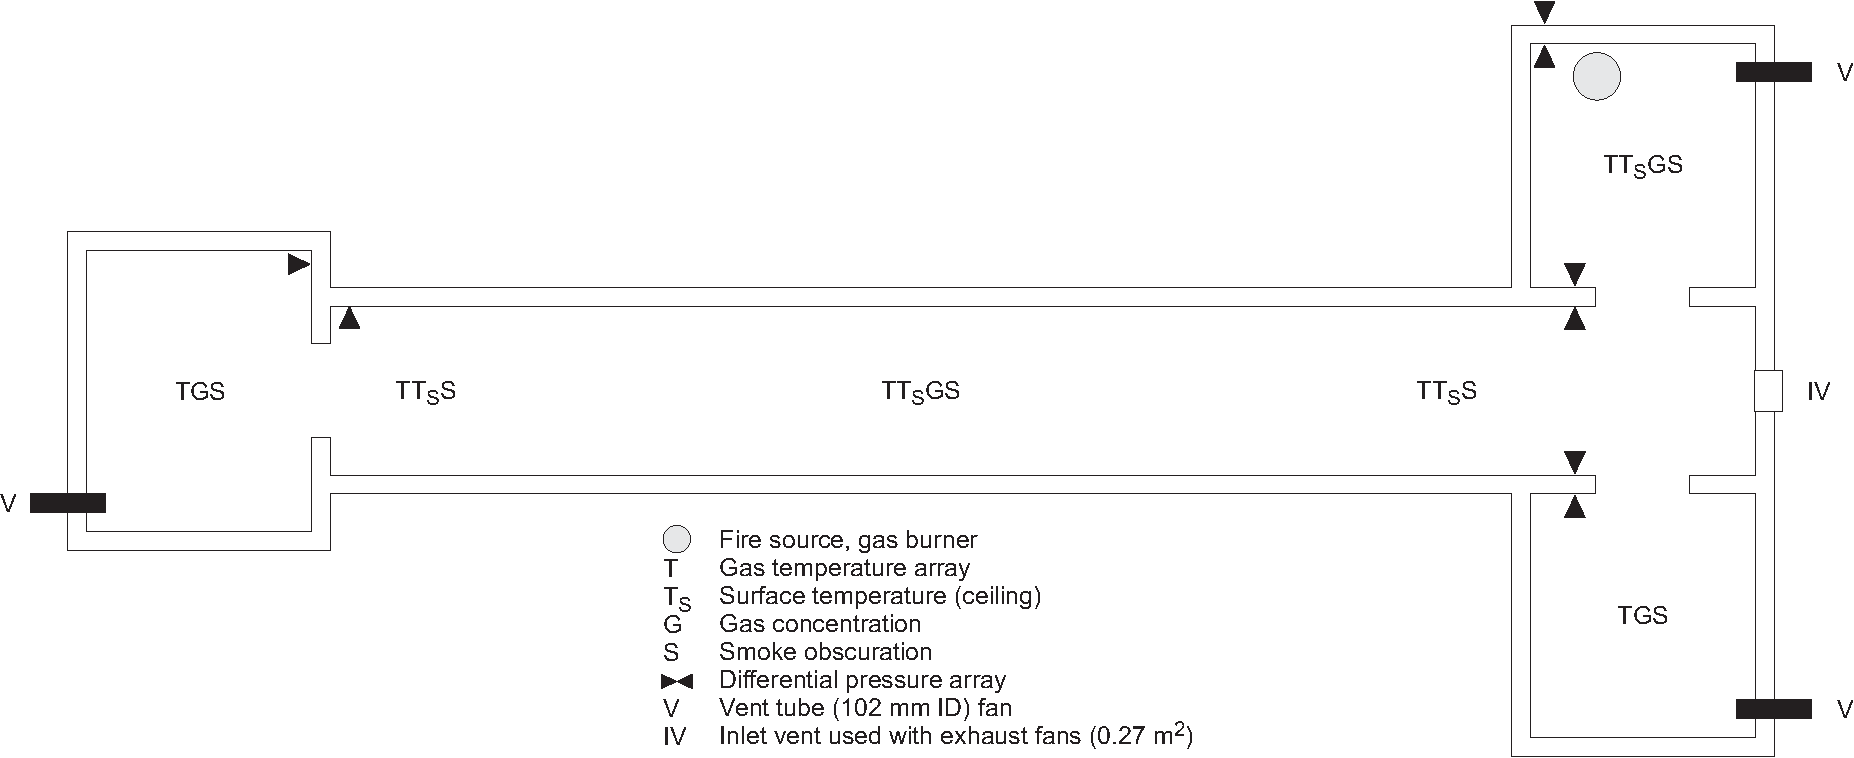
\includegraphics[width=6.0in]{FIGURES/FM_NBS/FMSummary}\\
\end{tabular}
\end{center}
\caption{Overview of the {F}actory {M}utual Four Room test series.}
 \label{fig:FMSummary}
\end{figure}

Room 3, located opposite the burn room, measured 3.65 m deep x 3.64 m wide x 2.45 m high; a door, measuring 0.88 m by 2.02 m high, was centered on the front wall (opening to the corridor). Room 4, located at the opposite end of the corridor, measured 3.65 m deep x 3.65 m wide x 2.43 m high and had a 0.88 m by 2.02 m high door centered on the front wall (opening to the corridor); an observation alcove, measuring 1.28 m by 0.86 m by 1.99 m high, was located in the front corner of room 4. Each room was equipped with a 102~mm inside diameter vent tube with a 61 mm inside diameter orifice meter and thermocouple, with option of exhaust fan (tube centered 0.27 m from the floor and 0.17 m from the closest parallel wall). An inlet vent (0.29 m$^2$) used with exhaust fans was centered 0.43 m above the floor at the end of the corridor between the burn room and room 3. When not in use, the inlet vent was sealed with a gypsum board cover taped in place.

The target room doors were commercial fire doors (wood-faced composite doors with calcium silicate cores, 14 h rated) mounted on 16 gage steel frames. The burn room door was fabricated from 12.7 mm calcium silicate, mounted in a steel frame lined with calcium silicate. Details of the doors and the spacings (cracks) are given in the original reference \cite{Heskestad:1986}.

Gypsum wallboard, 12.7 mm thick, on wood studs was used throughout the experimental facility. In addition, the walls and ceiling of the burn room were overlaid with calcium silicate, also 12.7 mm thick, to harden against repeated fire exposure. The existing concrete floor of the test building was used.

Two types of fire sources were used: 1) steady propylene fires at 56 kW on a 0.30 m diameter sand burner and 522 kW on a 0.91 m diameter burner and 2) propylene fires on the 0.91 m diameter burner programmed under computer control to grow with the square of time, exceeding 1 MW in 1, 2, 4, or 8 min.

The 0.91 m diameter, 0.58 in high propylene burner was used for most of the tests. Its design consisted of a 12 gage steel container with a gas distributor near the bottom, filled with gravel to a 67 percent height, where there was wire mesh screen, and coarse sand to the full height of the burner. The 0.30 m diameter burner was a scaled-down version of similar design.

\section{FM / SNL Test Series}

The Factory Mutual and Sandia National Laboratories (FM/SNL) Test Series was a series of 25 fire tests conducted in 1985 for the NRC by Factory Mutual Research Corporation (FMRC), under the direction of Sandia National Laboratories (SNL).  The primary purpose of these tests was to provide data with which to validate computer models for various types of NPP compartments.  The experiments were conducted in an enclosure measuring 18 m x 12 m x 6 m, constructed at the FMRC fire test facility in Rhode Island.  Figure \ref{fig:FMSNL_Detailed} shows detailed schematic drawings of the compartment from various perspectives.  The FM/SNL test series is described in detail, including the types and locations of measurement devices, as well as some results in References \cite{Nowlen:1987, Sandia:1989}.  Six of
the experiments were conducted with a full-scale control room mock-up in place. Parameters varied
during the experiments included fire intensity, enclosure ventilation rate, and fire location.
The current guide uses data from nineteen experiments (Tests 1-17, 21, and 22).
In these tests,  propylene gas burners, heptane pools, and methanol pools were used as fire sources.
Table~\ref{FM_SNL_Matrix} lists the test parameters.

The following information was provided by the test director,
Steve Nowlen of Sandia National Laboratory. In particular, Tests 4, 5, and 21 were given extra attention.
\begin{description}
\item[Heat Release Rate:] The HRR was determined using oxygen consumption calorimetry in the exhaust stack with
a correction applied for the carbon dioxide in the upper layer of the compartment. The
uncertainty of the fuel mass flow was not documented. Several tests selected for this study had
the same target peak heat release rate of 516~kW following a 4~min ``t-squared'' growth
profile. The test report contains time histories of the measured HRR, for which the average,
sustained HRR following the ramp up for Tests 4, 5, and 21 have been estimated as 510~kW, 480~kW, and 470~kW, respectively.
Once reached, the peak HRR was maintained essentially constant
during a steady-burn period of 6~min in Tests~4 and 5, and 16~min in Test~21. Note that in Test 21, Nowlen reports a
``significant'' loss of effluent from the exhaust hood that could lead to an under-estimate of the HRR towards the end of the experiment.
\item[Radiative Fraction:] The radiative fraction was not measured during the experiment, but
in this study it is assumed to equal 0.35, which is typical for a smoky hydrocarbons.
It was further assumed that the radiative fraction was about the same in
Test~21 as the other tests, as fuel burning must have occurred outside of the electrical cabinet in
which the burner was placed.
\item[Measurements:] Four types of measurements were conducted during the FM/SNL test series that are used in the
current model evaluation study, including the HGL temperature and depth, and the ceiling jet and
plume temperatures. Aspirated thermocouples (TCs) were used to make all of the temperature
measurements. Generally, aspirated TC measurements are preferable to bare-bead TC measurements,
as systematic radiative exchange measurement error is reduced.
\item[HGL Depth and Temperature:] Data from all of the vertical TC trees were used when reducing
the HGL height and temperature. For the majority of the tests, Sectors 1, 2, and 3 were used,
all weighted evenly. For Tests 21 and 22, Sectors 1 and 3 were used, evenly weighted. Sector 2 was
partially within the fire plume.
\end{description}

\begin{table}[h!]
\caption{Summary of FM/SNL Experiments.}
\begin{center}
\begin{tabular}{|c|c|c|c|c|c|c|}
\hline
Test    &  Fuel             & Nominal Peak  & Fire          & Ventilation       & Room                  & Used in  \\
No.     &  Type             & HRR (kW)      & Position      & Rate (ach)        & Configuration         & Guide?      \\ \hline \hline
1       & Propylene Burner  &     516       & Center        & 10                & Empty                 &        Yes \\ \hline
2       & Propylene Burner  &     516       & Center        & 10                & Empty                 &        Yes \\ \hline
3       & Propylene Burner  &    2000       & Center        & 10                & Empty                 &        Yes \\ \hline
4       & Propylene Burner  &     516       & Center        & 1                 & Empty                 &        Yes \\ \hline
5       & Propylene Burner  &     516       & Center        & 10                & Empty                 &        Yes \\ \hline
6       & Heptane Pool      &     500       & Wall          & 1                 & Empty                 &        Yes \\ \hline
7       & Propylene Burner  &     516       & Center        & 1                 & Empty                 &        Yes \\ \hline
8       & Propylene Burner  &    1000       & Center        & 1                 & Empty                 &        Yes \\ \hline
9       & Propylene Burner  &    1000       & Center        & 8                 & Empty                 &        Yes \\ \hline
10      & Heptane Pool      &    1000       & Wall          & 4.4               & Empty                 &        Yes \\ \hline
11      & Methanol Pool     &     500       & Wall          & 4.4               & Empty                 &        Yes \\ \hline
12      & Heptane Pool      &    2000       & Wall          & 4.4               & Empty                 &        Yes \\ \hline
13      & Heptane Pool      &    2000       & Wall          & 8                 & Empty                 &        Yes \\ \hline
14      & Methanol Pool     &     500       & Wall          & 1                 & Empty                 &        Yes \\ \hline
15      & Heptane Pool      &    1000       & Wall          & 1                 & Empty                 &        Yes \\ \hline
16      & Heptane Pool      &    500       & Corner        & 1                 & Empty                 &        Yes \\ \hline
17      & Heptane Pool      &    500       & Corner        & 10                & Empty                 &         No \\ \hline
18      &  PMMA Slab        &    1000       & Wall          & 1                 & Empty                 &         No \\ \hline
19      & Heptane Pool      &    1000       & Center        & 1                 & Furnished             &         No \\ \hline
20      & Heptane Pool      &    1000       & Corner        & 8                 & Furnished             &        Yes \\ \hline
21      & Propylene Burner  &     500       & Cabinet       & 1                 & Furnished             &        Yes \\ \hline
22      & Propylene Burner  &    1000       & Cabinet       & 1                 & Furnished             &         No \\ \hline
23      & Qualified Cable   &        N/A    & Cabinet       & 1                 & Furnished             &         No \\ \hline
24      & Unqualified Cable &        N/A    & Cabinet       & 1                 & Furnished             &         No \\ \hline
25      & Unqualified Cable &        N/A    & Cabinet       & 8                 & Furnished             &         No \\ \hline
\end{tabular}
\end{center}
\label{FM_SNL_Matrix}
\end{table}

\begin{figure}
\begin{center}
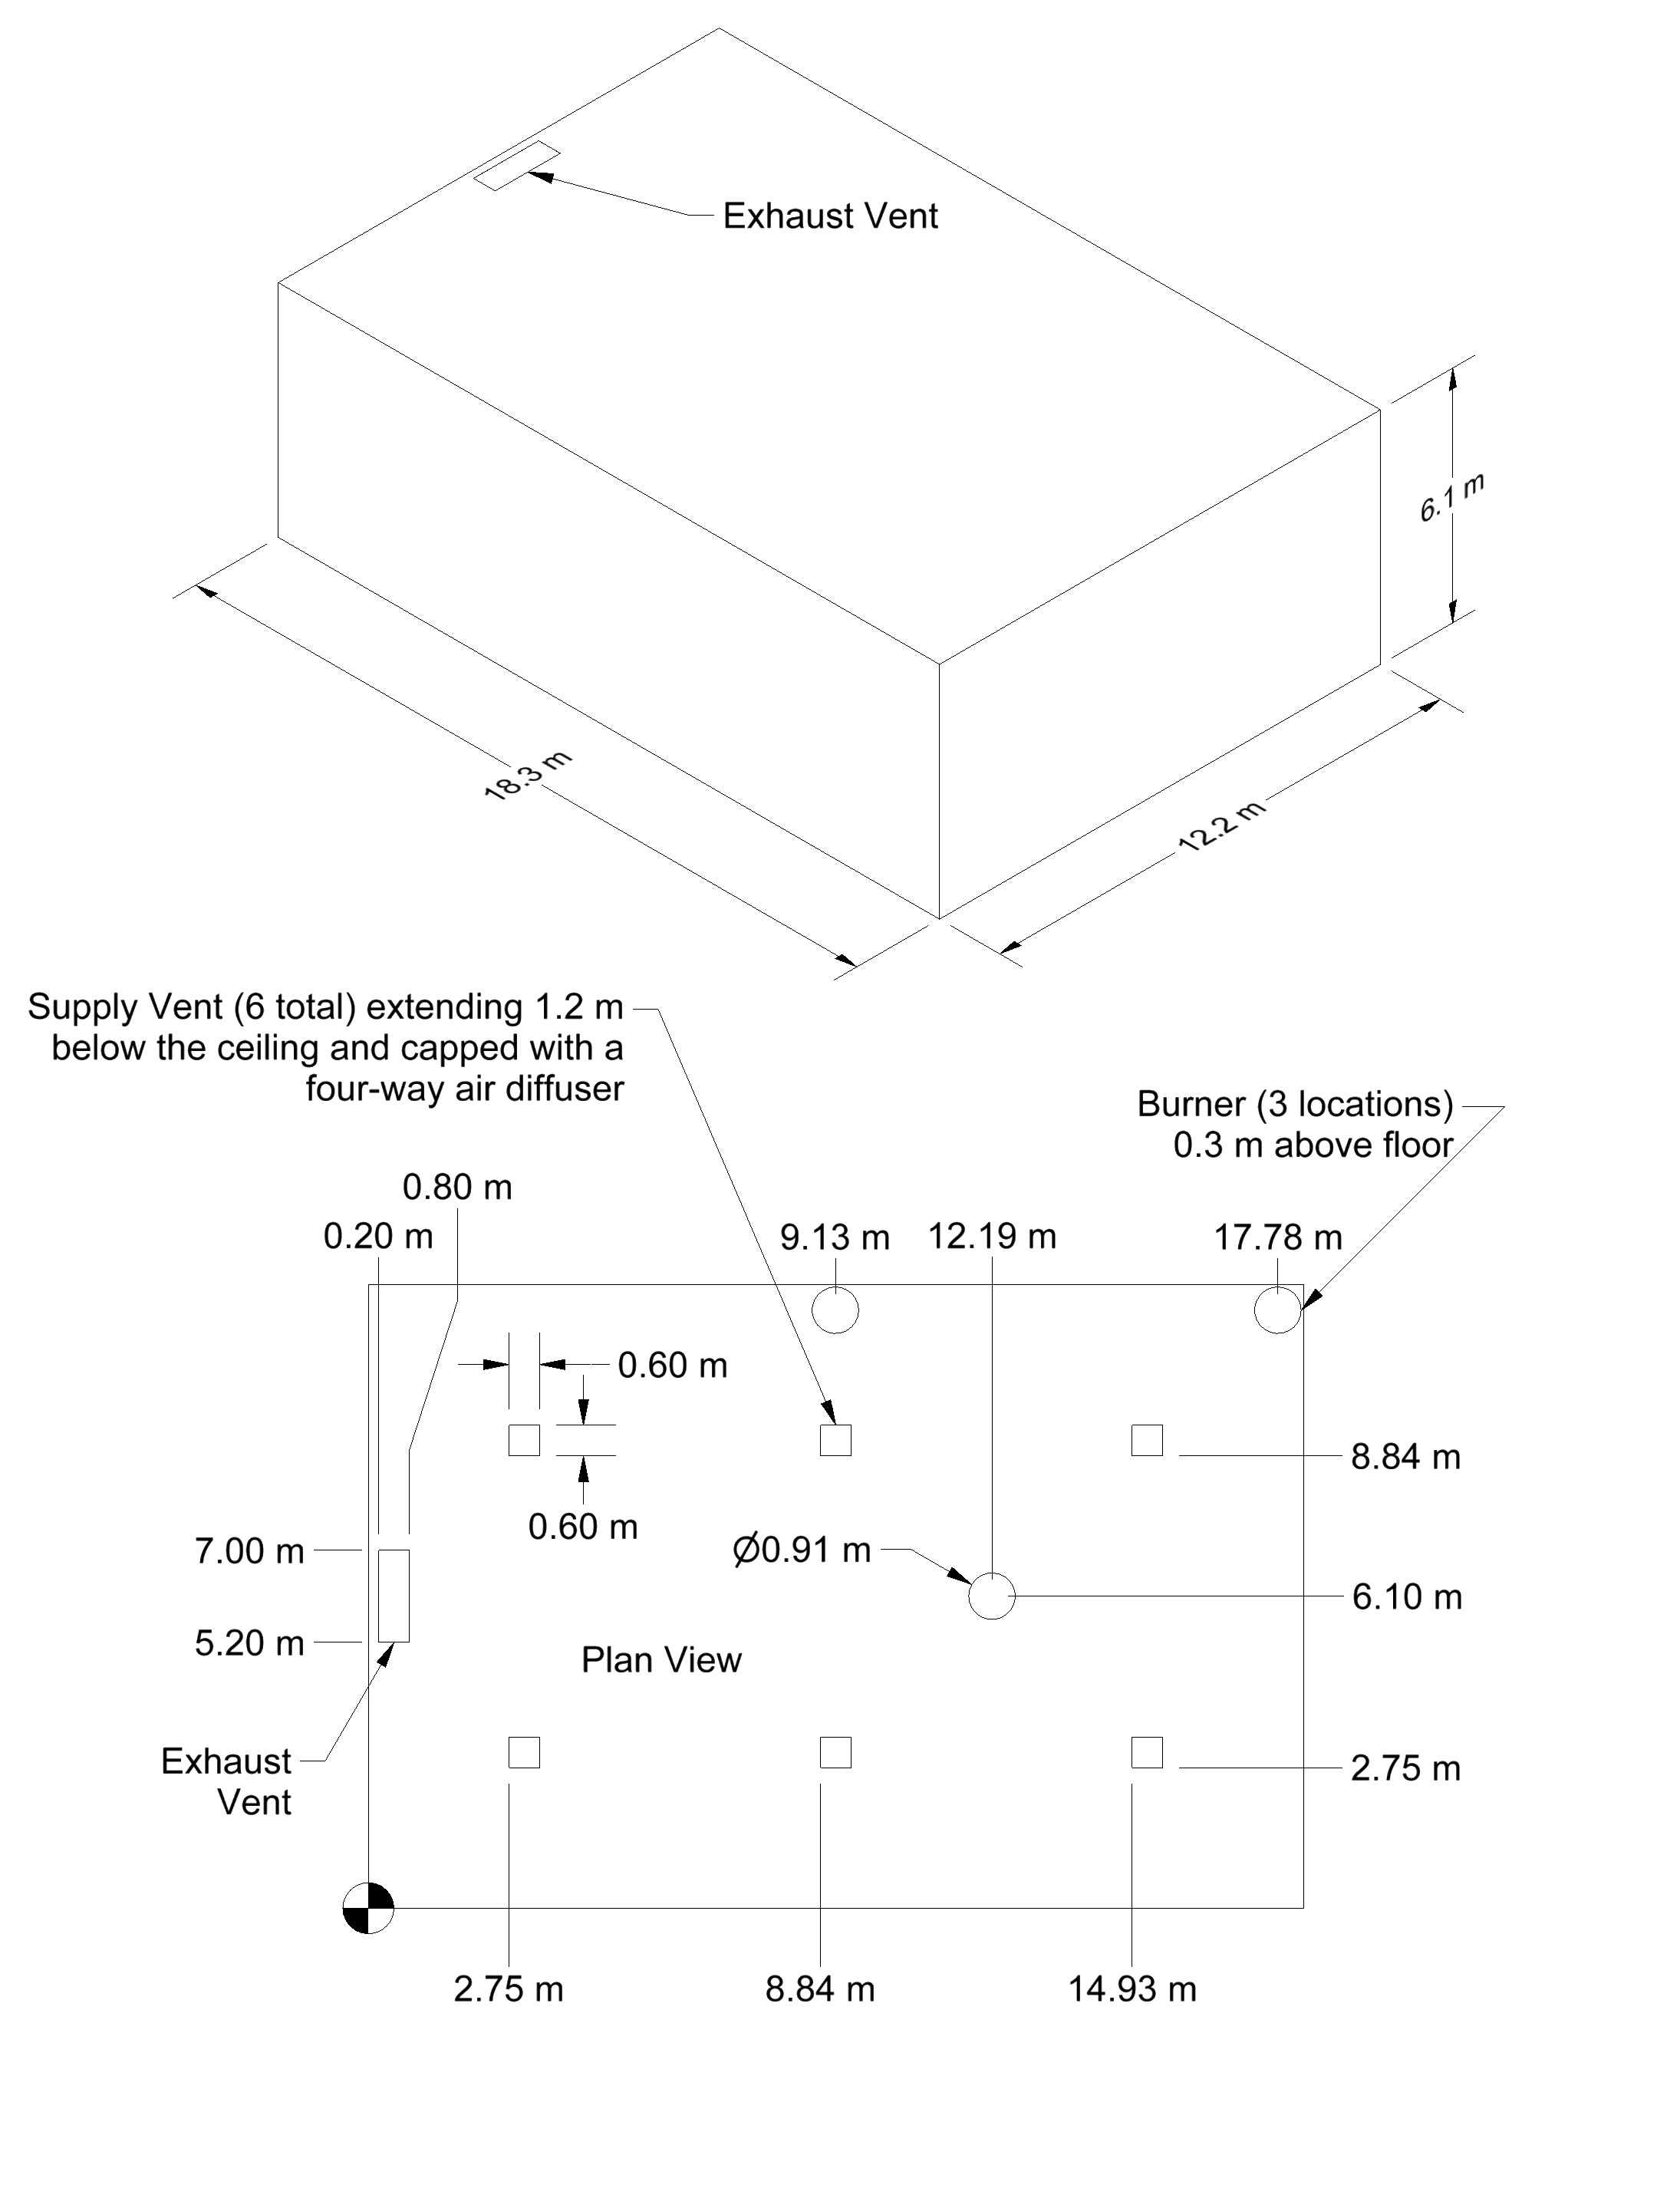
\includegraphics[width=6.5in]{FIGURES/FM_SNL/FM_SNL_Drawing}\\
\end{center}
\caption{Detailed plan, side, and perspective schematic drawings of the FM/SNL experimental arrangement, including the supply and exhaust ducts, and the fuel pan.}
 \label{fig:FMSNL_Detailed}
\end{figure}

All of the tests involved forced ventilation to simulate typical nuclear power plant installation practices.

\begin{figure}[\figoptions{t}]
\begin{center}
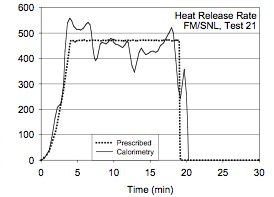
\includegraphics[width=3.0in]{FIGURES/FM_SNL/FMSNL_HRR}\\
\end{center}
\caption{Prescribed (dotted line) and measured (solid line) heat release rate as a function of time during Test 21 of the FM/SNL test series}
 \label{fig:FMSNL_HRR}
\end{figure}

\section{iBMB Compartment Tests}

A series of small compartment kerosene pool fire experiments, conducted at the
Institut f\"ur Baustoffe, Massivbau und Brandschutz (iBMB) of Braunschweig University of
Technology in Germany in 2004 \cite{Klein-Helbetaling:2005}.  The results from Test 1 were
considered here.  These experiments involved relatively large fires in a relatively small (3.6 m x 3.6 m x 5.7 m) concrete enclosure. Figure  \ref{fig:iBMB_Pool_Detailed} shows plan, side and perspective schematic drawings
of the experimental arrangement, including the location of the fuel pan, which was located at the
center of the compartment.

\begin{figure}
\begin{center}
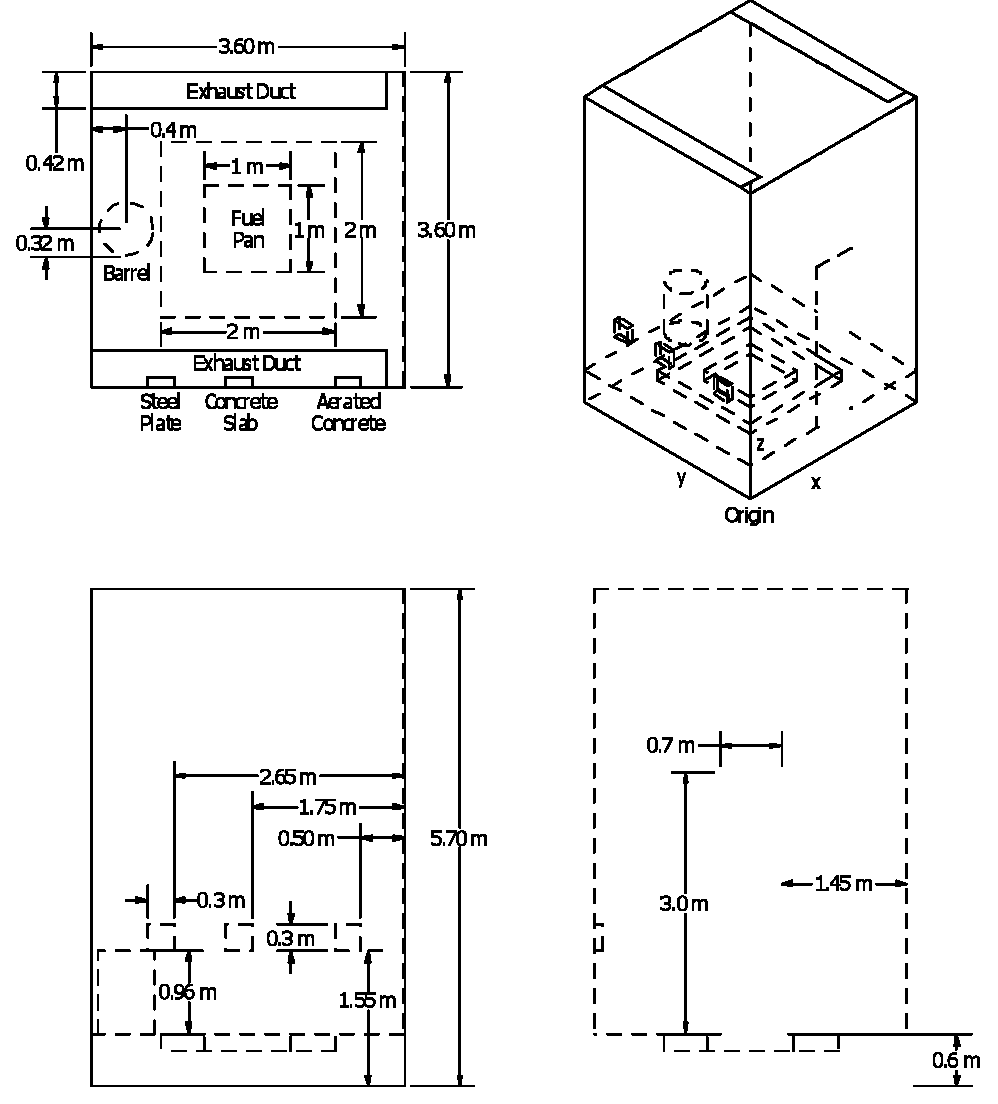
\includegraphics[width=6.5in]{FIGURES/iBMB/iBMB_Pool}\\
\end{center}
\caption{Detailed plan, side, and perspective schematic drawings of the iBMB pool fire experimental arrangement.}
 \label{fig:iBMB_Pool_Detailed}
\end{figure}

 Only a portion of Test 1 was selected for consideration in the present study, because a significant amount of data was lost in Test 2, and the measured ${\dQ}$  during Test 3 exhibited significant amounts of fluctuation. Five types of measurements that were conducted during the test series were used in the model evaluation reported here.  These included the HGL temperature and depth, the temperature of targets and compartment surfaces, and heat flux. In addition, figure \ref{fig:iBMB_HRR} shows the heat release rate for Test 1, which was estimated from a mass loss rate measurement.  In this calculation, the heat of combustion and the combustion efficiency were taken as 42.8~MJ/kg and 1, respectively, as suggested by Refs.~\cite{NRCNUREG1824, Riese:2004}.  There were several reported difficulties in measuring the mass loss rate, including data loss due to an instrument malfunction and significant fluctuations in the measured mass loss rate. Due to these measurement issues and because the combustion efficiency was not well-characterized, the ${\dQ}$ uncertainty was assigned a relatively large expanded uncertainty of $\pm$ 25~\%~\cite{NRCNUREG1824}.

 \begin{figure}
\begin{center}
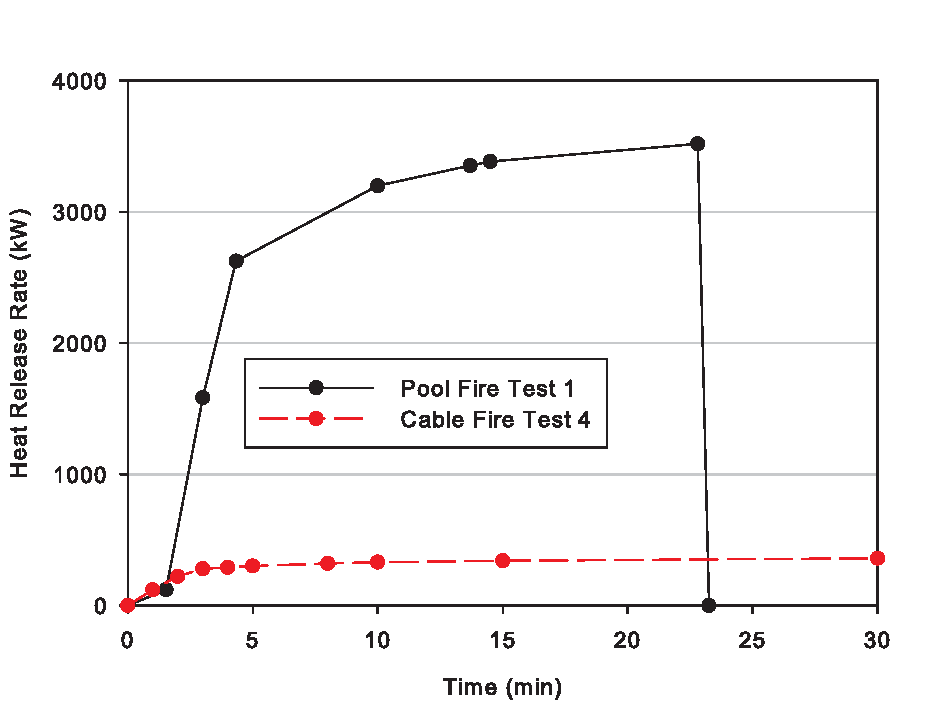
\includegraphics[width=4.0in]{FIGURES/iBMB/iBMB_HRR}\\
\end{center}
\caption{Estimated heat release rate for the iBMB fire experiments.}
 \label{fig:iBMB_HRR}
\end{figure}

A second series of fire experiments in 2004, conducted under the International Collaborative Fire Model Project (ICFMP) involved realistically routed cable
trays inside the same concrete enclosure at iBMB \cite{Riese:2004}. The compartment was configured slightly differently with a ceiling height of 5.6 m. A schematic diagram from plan, side, and perspective views of the experimental arrangement is shown in figure \ref{fig:iBMB_Cable_Detailed}. Six types of measurements conducted during the test series were used in the evaluation conducted here, including the HGL temperature and depth, oxygen gas concentration, the temperature of targets and compartment surfaces, and heat flux.

\begin{figure}
\begin{center}
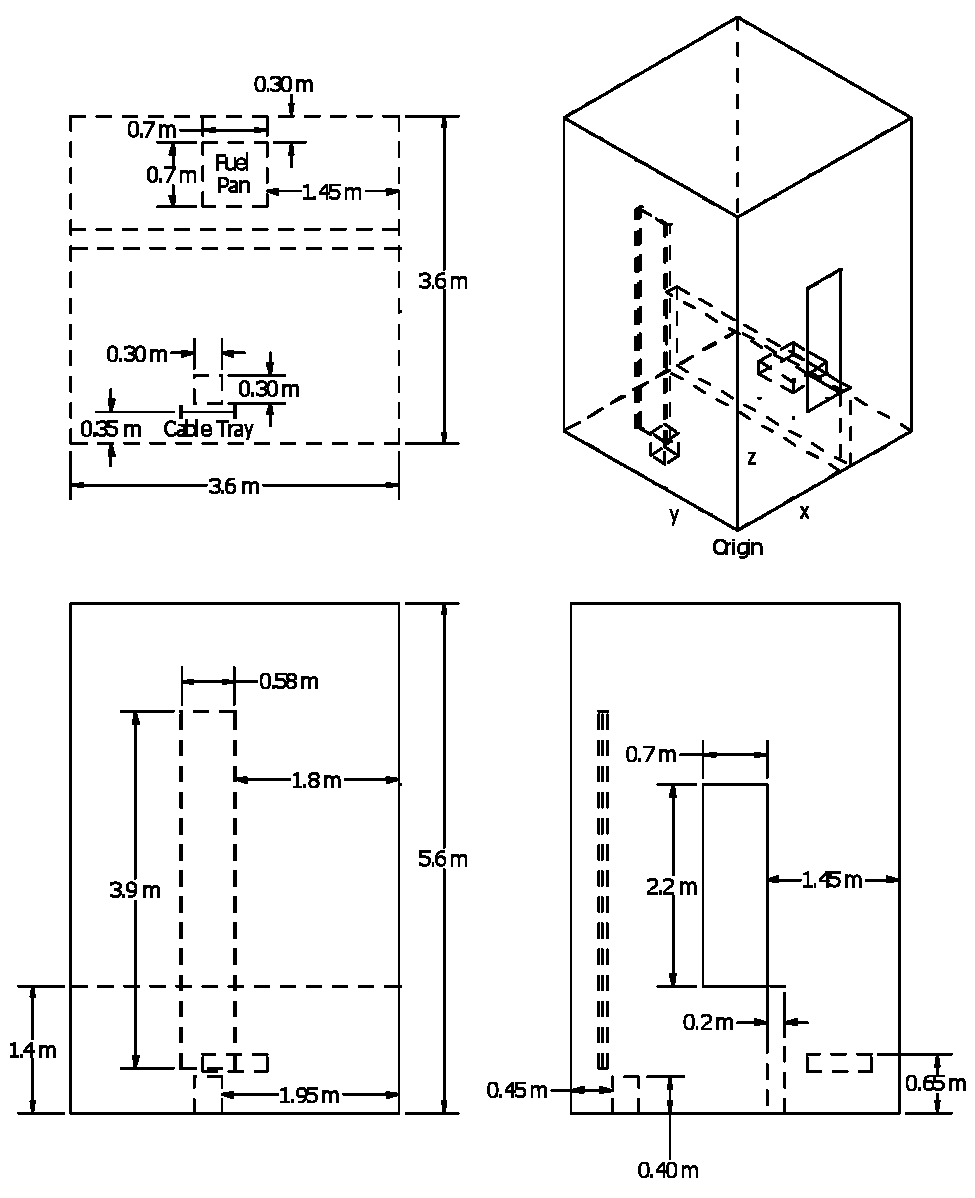
\includegraphics[width=6.5in]{FIGURES/iBMB/iBMB_Cable}\\
\end{center}
\caption{Detailed plan, side, and perspective schematic drawings of the iBMB cable fire experimental arrangement.}
 \label{fig:iBMB_Cable_Detailed}
\end{figure}

The results of four tests were
available, of which one has been used in the current study.
These tests were conducted primarily for the evaluation of cable ignition and flame spread.
The results were erratic, and no replicate experiments were performed. Given the primitive
nature of the ignition and spread algorithms within the models, it was decided that only
a qualitative analysis would be possible with the data from three of the four experiments.
However, in one experiment, the first 20 minutes involved a fairly well-characterized ethanol
pool fire burning on the opposite side of the compartment from the cable tray. This part of
the experiment has been used as part of the model evaluation.

The first part of the test consisted of preheating the cable trays in the room with a 1 m$^2$ round pan on the floor filled with ethanol (ethyl alcohol) used as the preheating source.  At 30 min, a propane gas burner was used as the fire source; this was not considered because only the first 20 min of the test was used in this validation study.
Exhaust products were collected in an exhaust duct and the $\dQ$  was measured using the oxygen calorimetry.  For the purpose of this study, the measured $\dQ$ was used as direct input to the various fire models.  The first 20 min of data were used for the model evaluation. After 20 min, the  $\dQ$ became relatively noisy.  Figure \ref{fig:iBMB_HRR} shows the HRR. The relative combined expanded uncertainty was assigned a value of $\pm$15 \%, consistent with typical values of this parameter \cite{NRCNUREG1824}.

\section{LLNL Enclosure Tests}

Sixty-four enclosure fire tests were conducted by Lawrence Livermore National Laboratory (LLNL) in 1986 to study the effects of ventilation on enclosure fires~\cite{Foote:LLNL1986}. The test
enclosure was 6~m long, 4~m wide, and 4.5~m high. It contained a methane rock burner which was placed in the center of the space. For most of the tests the burner was placed on the
floor. The fires varied in size from 50~kW to 400~kW. The burner was 0.57~m in diameter and 0.23~m height.

The door (2.06 m high by 0.76 m wide) was closed and sealed for most tests, and air was pulled through the space at rates varying from 100 to 500~g/s. In some tests the enclosure included a plenum space, where
make-up air could be injected from above or below. The test matrix is listed in Table~\ref{LLNL_Matrix}.

\begin{table}[p]
\caption[Summary of LLNL Enclosure Experiments]{Summary of LLNL Enclosure Experiments.}
\begin{center}
\begin{tabular}{|c|c|c|c|c|c||c|c|c|c|c|c|}
\hline
Test & Room    & $h_0$ &  $\dot{Q}$ & $\dot{m}$ & $T_\infty$  &   Test & Room    & $h_0$ &  $\dot{Q}$ & $\dot{m}$ & $T_\infty$  \\
No.  & Config. & m     &  kW        & g/s       & $^\circ$C   &   No.  & Config. & m     &  kW        & g/s       & $^\circ$C   \\ \hline \hline
1    & TL      & 0     & 200        & 0         & 23          &   33   & PH      & 0     & 100        & 200       & 23          \\ \hline
2    & TL      & 0     & 200        & 0         & 27          &   34   & PH      & 0     & 100        & 300       & 34          \\ \hline
3    & TL      & 0     & 400        & 0         & 27          &   35   & PH      & 0     & 100        & 400       & 22          \\ \hline
4    & TL      & 0     & 300        & 0         & 24          &   36   & PH      & 0     & 100        & 500       & 29          \\ \hline
5    & TL      & 0     & 50         & 0         & 28          &   37   & PH      & 0     & 200        & 100       & 20          \\ \hline
6    & TL      & 0     & 100        & 0         & 29          &   38   & PH      & 0     & 200        & 300       & 29          \\ \hline
7    & TL      & 0     & 100        & 0         & 35          &   39   & PH      & 0     & 250        & 100       & 18          \\ \hline
8    & TL      & 0     & 200        & 0         & 35          &   40   & PH      & 0     & 200        & 400       & 28          \\ \hline
9    & TL      & 0     & 200        & 500       & 33          &   41   & PH      & 0     & 150        & 100       & 20          \\ \hline
10   & TL      & 0     & 200        & 100       & 28          &   42   & PHE     & 2     & 200        & 180       & 30          \\ \hline
11   & TL      & 0     & 200        & 200       & 18          &   43   & PHE     & 2     & 200        & 0         & 32          \\ \hline
12   & TL      & 0     & 200        & 300       & 21          &   44   & PHE     & 1     & 200        & 180       & 19          \\ \hline
13   & TL      & 0     & 200        & 400       & 28          &   45   & PHE     & 1     & 200        & 0         & 30          \\ \hline
14   & TL      & 0     & 200        & 400       & 28          &   46   & PHE     & 0.6   & 200        & 180       & 19          \\ \hline
15   & TL      & 0     & 100        & 300       & 24          &   47   & PHE     & 0.6   & 200        & 0         & 19          \\ \hline
16   & TL      & 0     & 200        & 300       & 21          &   48   & PHE     & 0.3   & 200        & 0         & 21          \\ \hline
17   & PL      & 0     & 200        & 500       & 26          &   49   & PHE     & 0.3   & 200        & 180       & 26          \\ \hline
18   & PL      & 0     & 200        & 400       & 21          &   50   & PHE     & 1     & 200        & 180       & 21          \\ \hline
19   & PL      & 0     & 200        & 300       & 18          &   51   & PNE     & 1     & 200        & NAT       & 33          \\ \hline
20   & PL      & 0     & 200        & 200       & 16          &   52   & PN      & 0     & 200        & NAT       & 23          \\ \hline
21   & PL      & 0     & 200        & 100       & 23          &   53   & PHGS    & 0     & 200        & 185       & 33          \\ \hline
22   & PH      & 0     & 200        & 190       & 30          &   54   & PHGS    & 0     & 200        & 215       & 21          \\ \hline
23   & PH      & 0     & 200        & 215       & 28          &   55   & PN      & 0     & 100        & NAT       & 31          \\ \hline
24   & PH      & 0     & 200        & 205       & 26          &   56   & PHGW    & 0     & 200        & 190       & 20          \\ \hline
25   & PH      & 0     & 200        & 205       & 25          &   57   & PHGW    & 0     & 200        & 215       & 29          \\ \hline
26   & PH      & 0     & 200        & 500       & 24          &   58   & PHX     & 0     & 200        & 190       & 18          \\ \hline
27   & PH      & 0     & 200        & 100       & 23          &   59   & PHXE    & 1     & 200        & 190       & 24          \\ \hline
28   & PH      & 0     & 150        & 150       & 31          &   60   & PN      & 0     & 400        & NAT       & 22          \\ \hline
29   & PH      & 0     & 250        & 250       & 28          &   61   & TN      & 0     & 200        & NAT       & 31          \\ \hline
30   & PH      & 0     & 250        & 300       & 34          &   62   & TN      & 0     & 400        & NAT       & 22          \\ \hline
31   & PH      & 0     & 250        & 500       & 36          &   63   & TN      & 0     & 50         & NAT       & 28          \\ \hline
32   & PH      & 0     & 100        & 100       & 33          &   64   & TN      & 0     & 100        & NAT       & 17          \\ \hline
\end{tabular}
\end{center}
\begin{tabbing}
\hspace{0.7in} \= T \hspace{0.2in}  \= full compartment     \hspace{0.8in} \= N \hspace{0.2in} \= natural ventilation (door open) \\
               \> P                 \> plenum configuration                \> X                \> 3 ft extension on inlet opening \\
               \> L                 \> low inlet duct                      \> GS               \> grate on inlet, north/south configuration \\
               \> H                 \> high inlet duct                     \> GW               \> grate on inlet, east/west configuration \\
               \> E                 \> elevated fire, $h_0$
\end{tabbing}
\label{LLNL_Matrix}
\end{table}


\begin{figure}[\figoptions{b}]
\begin{center}
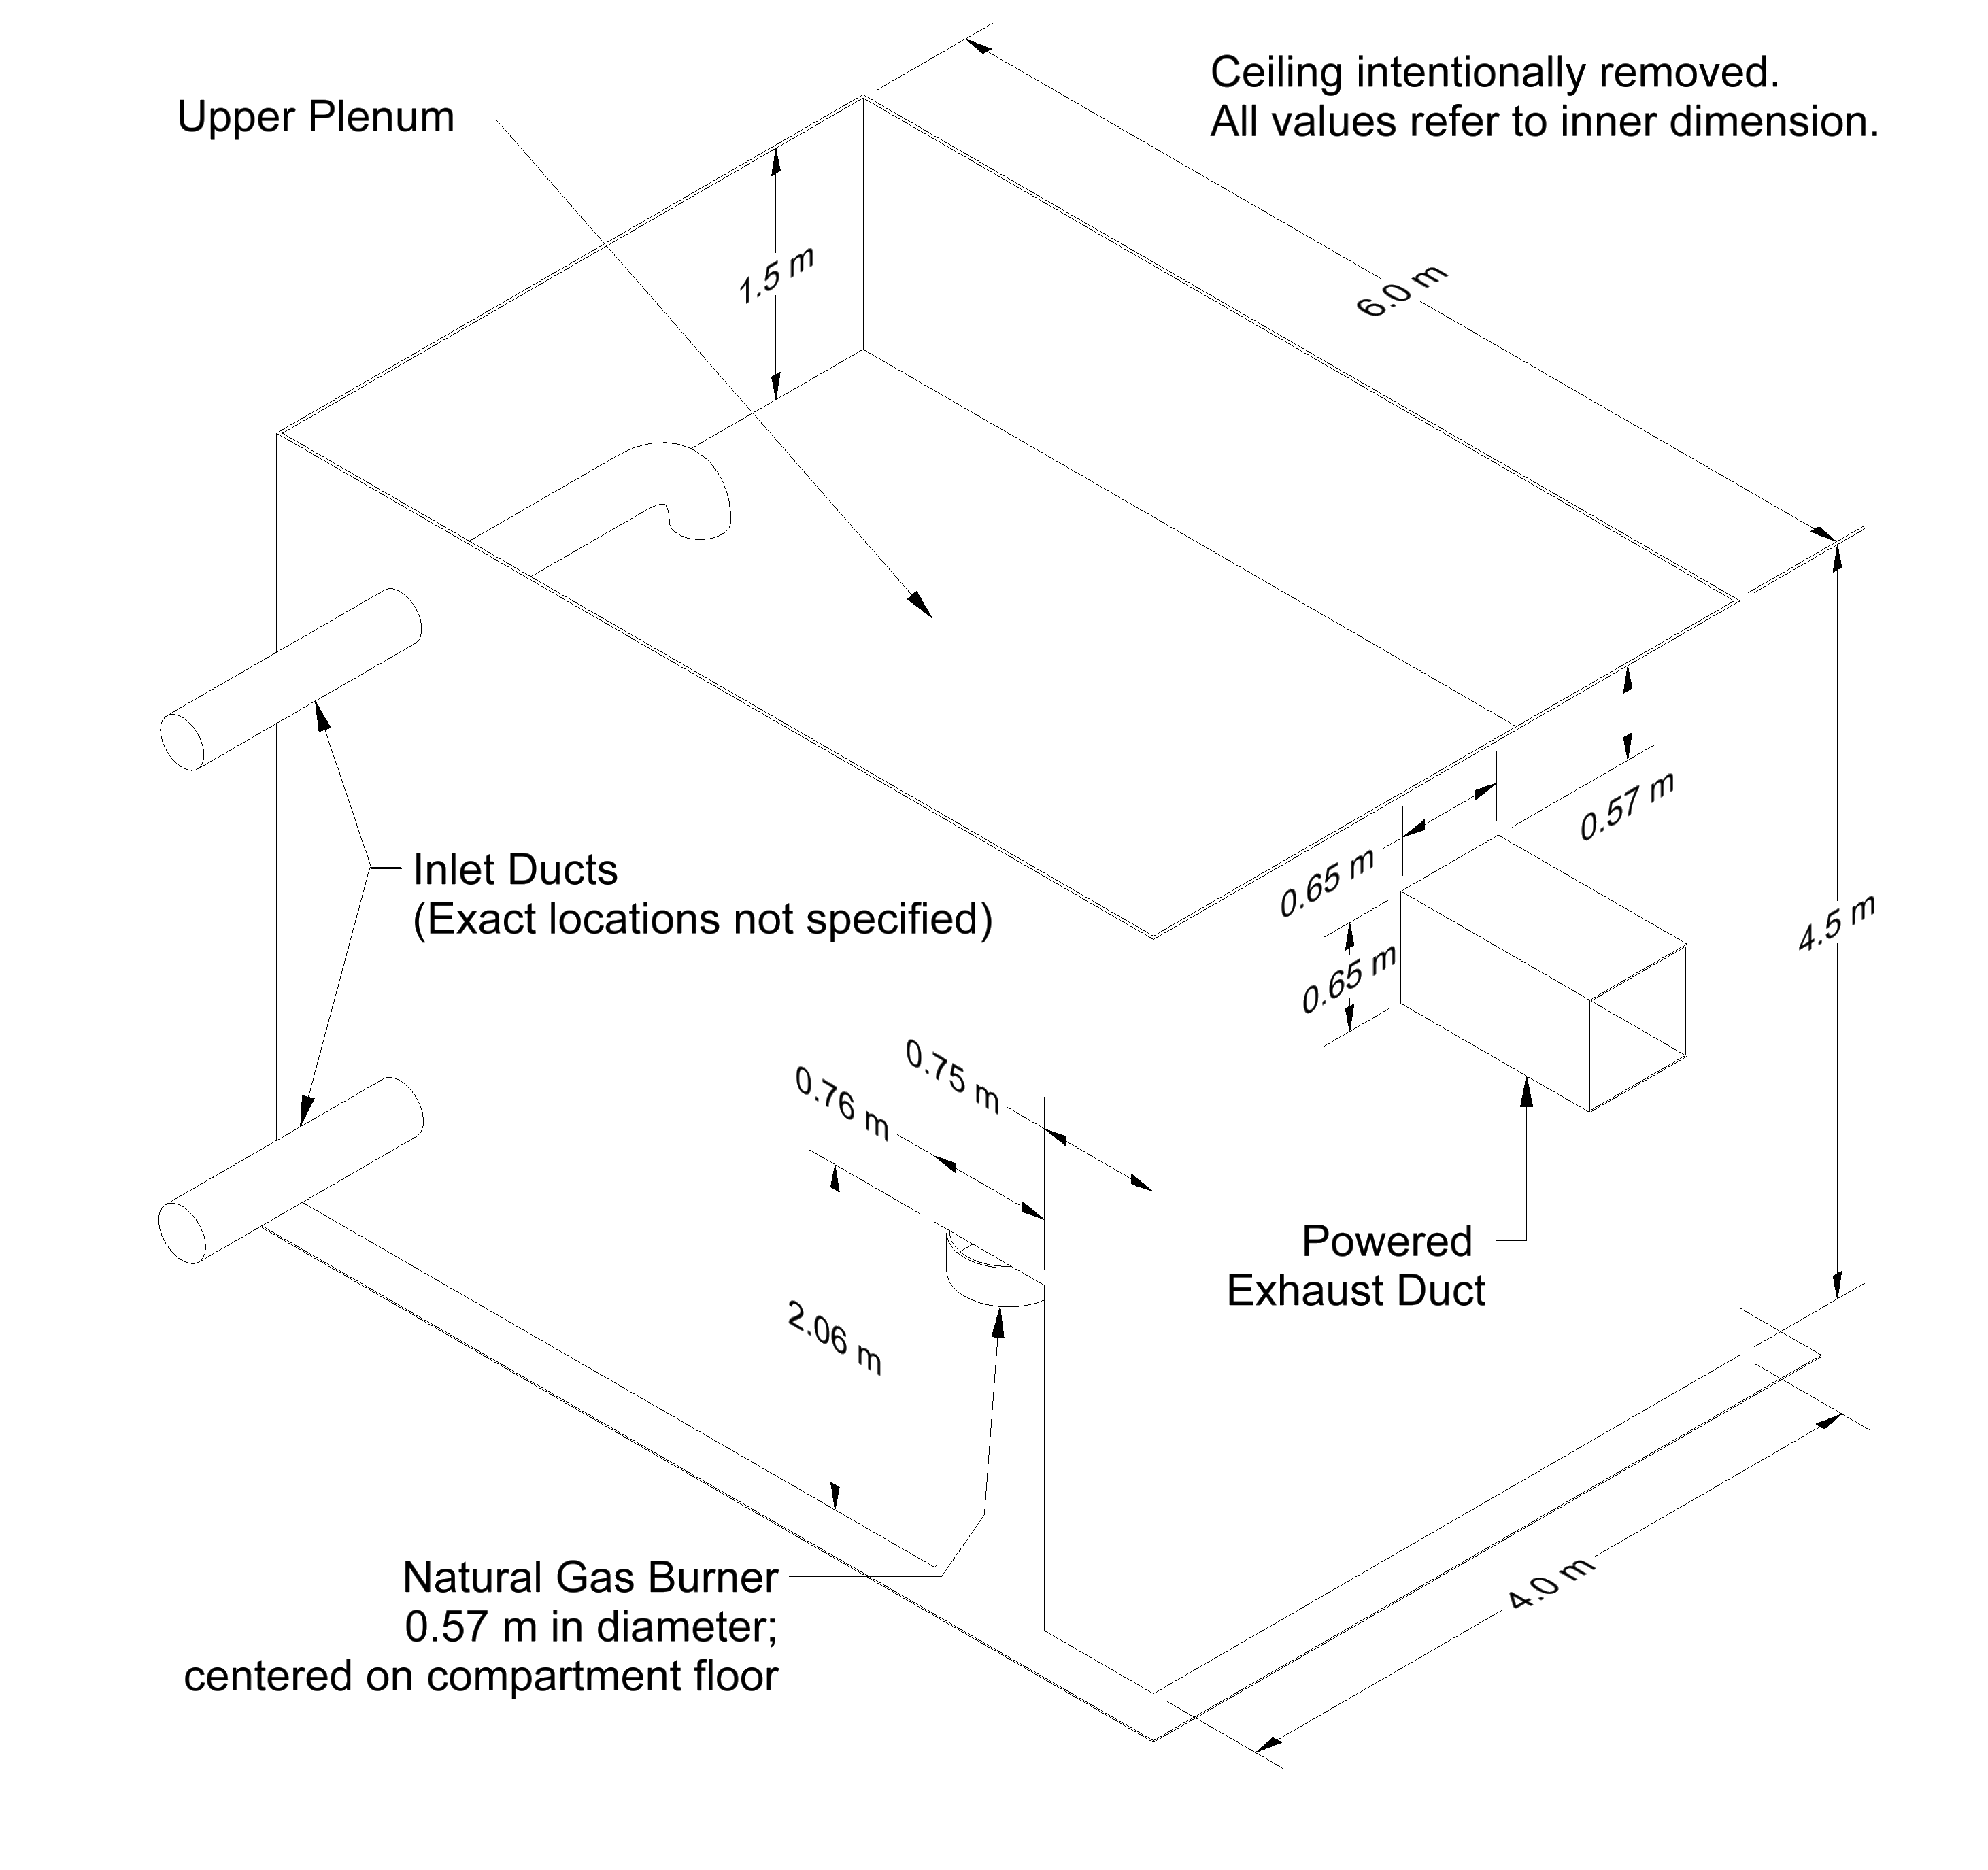
\includegraphics[width=6.5in]{FIGURES/LLNL_Enclosure/LLNL_Enclosure_Drawing}
\end{center}
\caption[Geometry of the LLNL Enclosure Experiments]{Geometry of the LLNL Enclosure Experiments.}
\label{LLNL_Enclosure_Drawing}
\end{figure}

\section{NBS Single Room Tests with Furniture}

These data describe a series of room fire tests using upholstered furniture items in a room of fixed size but with varying opening sizes and shapes \cite{Valid:Babrauskas_Flashover} conducted by the National Bureau of Standards (NBS, former name of NIST). It was selected for its well characterized and realistic fuel sources in a simple single-room geometry. In addition, the wide variation in opening size should provide challenges for current zone fire models. Peak fire size was about 2.9~MW with a total room volume of 21 m$^3$. A series of four single-room fire tests were conducted using upholstered furniture items for comparison with their free burning behavior, previously determined in a furniture calorimeter.  The experiments were conducted in a single room enclosure; ventilation to the room was provided by window openings of  varying sizes. The room was equipped with an instrumented exhaust collection system outside the window opening.

A second similar test series also utilized a single-room fire test with furniture as the fire source \cite{Lee:1985}. It expanded upon the first data set by adding the phenomenon of wall burning. Peak fire size was about 7 MW. The room size was similar to the first test series. Figure \ref{fig:NBSFurniture} illustrates the configuration for the two test series.

\begin{figure}[\figoptions{b}]
\begin{center}
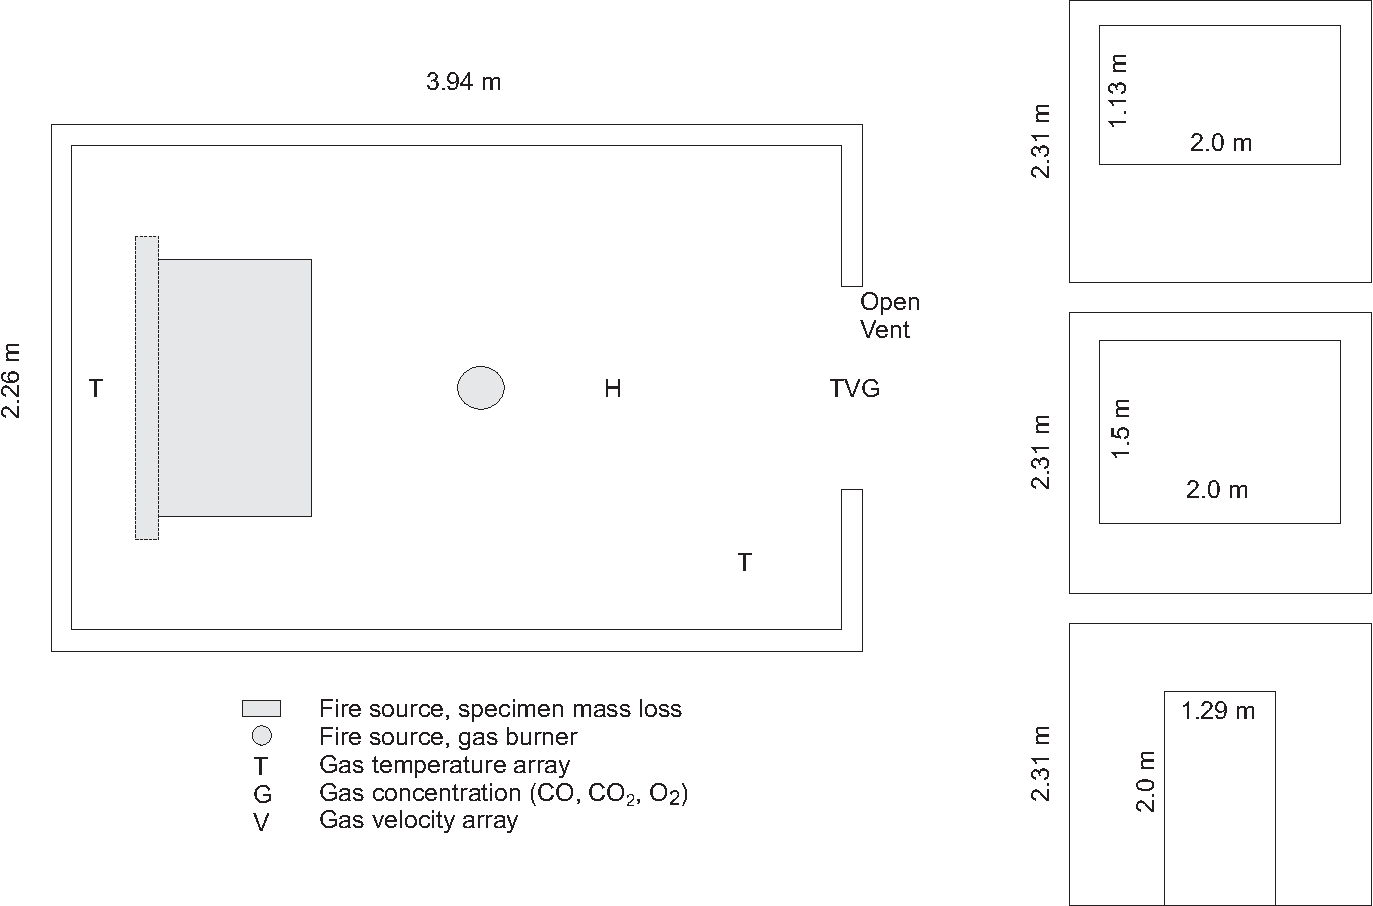
\includegraphics[width=5.0in]{FIGURES/NBS/NBSFurniture}\\
\end{center}
\caption[Plan and elevation view schematic of experimental room for NBS single room tests with furniture.]{Plan and elevation view schematic of experimental room for NBS single room tests with furniture. Note dotted lines on burning specimen indicates vertical surface for wall burning experiments.  Specimen and instrumentation placement are approximate.}
 \label{fig:NBSFurniture}
\end{figure}

\begin{figure}[\figoptions{b}]
\begin{center}
\includegraphics[width=5.0in]{FIGURES/NBS/NBS_Furniture_Test}\\
\end{center}
\caption[Burning specimen during NBS single room tests with furniture.]{Burning specimen during NBS single room tests with furniture.}
 \label{fig:NBSFurniturePix}
\end{figure}

The test furniture included a 28.3 kg armchair or a similar 40.0 kg love seat for the first test series. Both were of conventional wood frame construction and used polyurethane foam padding, made to minimum California State flammability requirements, and polyolefin fabric. A single piece of test furniture and igniting wastebasket were the only combustibles in the test room.

For the second test series, room furnishings consisted of a 1.37 m wide x 1.91 m long x 0.53 m high double bed, a 2.39 m X 0.89 m high headboard, and 0.51 m wide x 0.41 m deep x 0.63 m high night table. Both headboard and night table were fabricated from 12.7 mm thick plywood. The bedding was comprised of two pillows, two pillow cases, two sheets, and one blanket. The pillows had a polypropylene fabric with a polyester filling. The pillow cases and sheets were polyester-cotton. The blanket was acrylic material. The bedding was left in a "slept in" condition which was duplicated to the degree possible in each test. In all of the tests, the fire was started with match flame ignition of a 0.34 kg (240 mm x 140 mm x 240 mm high) wastebasket, filled with 0.41 kg of trash, positioned adjacent to the bed.

\section{NBS Multi-Compartment Test Series}

The National Bureau of Standards (NBS, former name of NIST) Multi-Compartment Test Series consisted of 45 fire tests representing 9 different sets of conditions were conducted in a three-room suite.  The experiments were conducted in 1985 and are described in detail in reference \cite{Peacock:1988}.  The suite consisted of two relatively small rooms, connected via a relatively long corridor. Total volume of the structure was approximately 100 m$^2$. The fire source, a gas burner, was located against the rear wall of one of the small compartments as seen in Figure \ref{fig:NBS_100kW_fire} for a 100 kW fire.  Figures \ref{fig:NBS_Summary} and \ref{fig:NBS_Detailed} presents the experimental arrangement in the form of plan, side and perspective schematic drawings of the compartments. Fire tests of 100 kW, 300 kW and 500 kW were conducted. For the current  study, three 100 kW fire experiments have been used, including Test 100A from Set 1, Test 100O from Set 2, and Test 100Z from Set 4. For the NBS Multi-room series, Tests 100A, 100O and 100Z were selected for study, because they were constructively used in a previous validation study [\cite{EPRI}, and because these tests had  the steadiest values of measured heat release rate during the steady burning period. The selected data are also available in Reference \cite{EPRI}.   Reference \cite{NRCNUREG1824} provides information used as model input for simulation of the NBS tests, including information on the compartment, the fire, the ventilation, and ambient conditions. The data in the NBS data set was acquired every 10 s with a 6 s time-average.  This time-averaging interval was somewhat smaller than all of the other experimental series, which were time-averaged over a 10 s interval.

\begin{figure}
\begin{center}
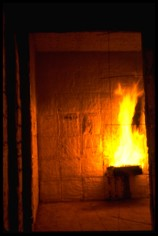
\includegraphics[width=2.0in]{FIGURES/NBS/NBS_100kW_fire}  \\
\end{center}
\caption{Photo of a 100 kW fire with the burner located against the rear wall of one of the small compartments in the NBS Multi-Compartment test Series.}
 \label{fig:NBS_100kW_fire}
\end{figure}

\begin{figure}[\figoptions{t}]
\begin{center}
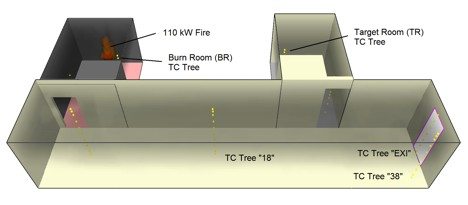
\includegraphics[width=5.0in]{FIGURES/NBS/NBS_Summary}\\
\end{center}
\caption{Overview of the NBS Test Configuration.}
 \label{fig:NBS_Summary}
\end{figure}

\begin{figure}[\figoptions{t}]
\begin{center}
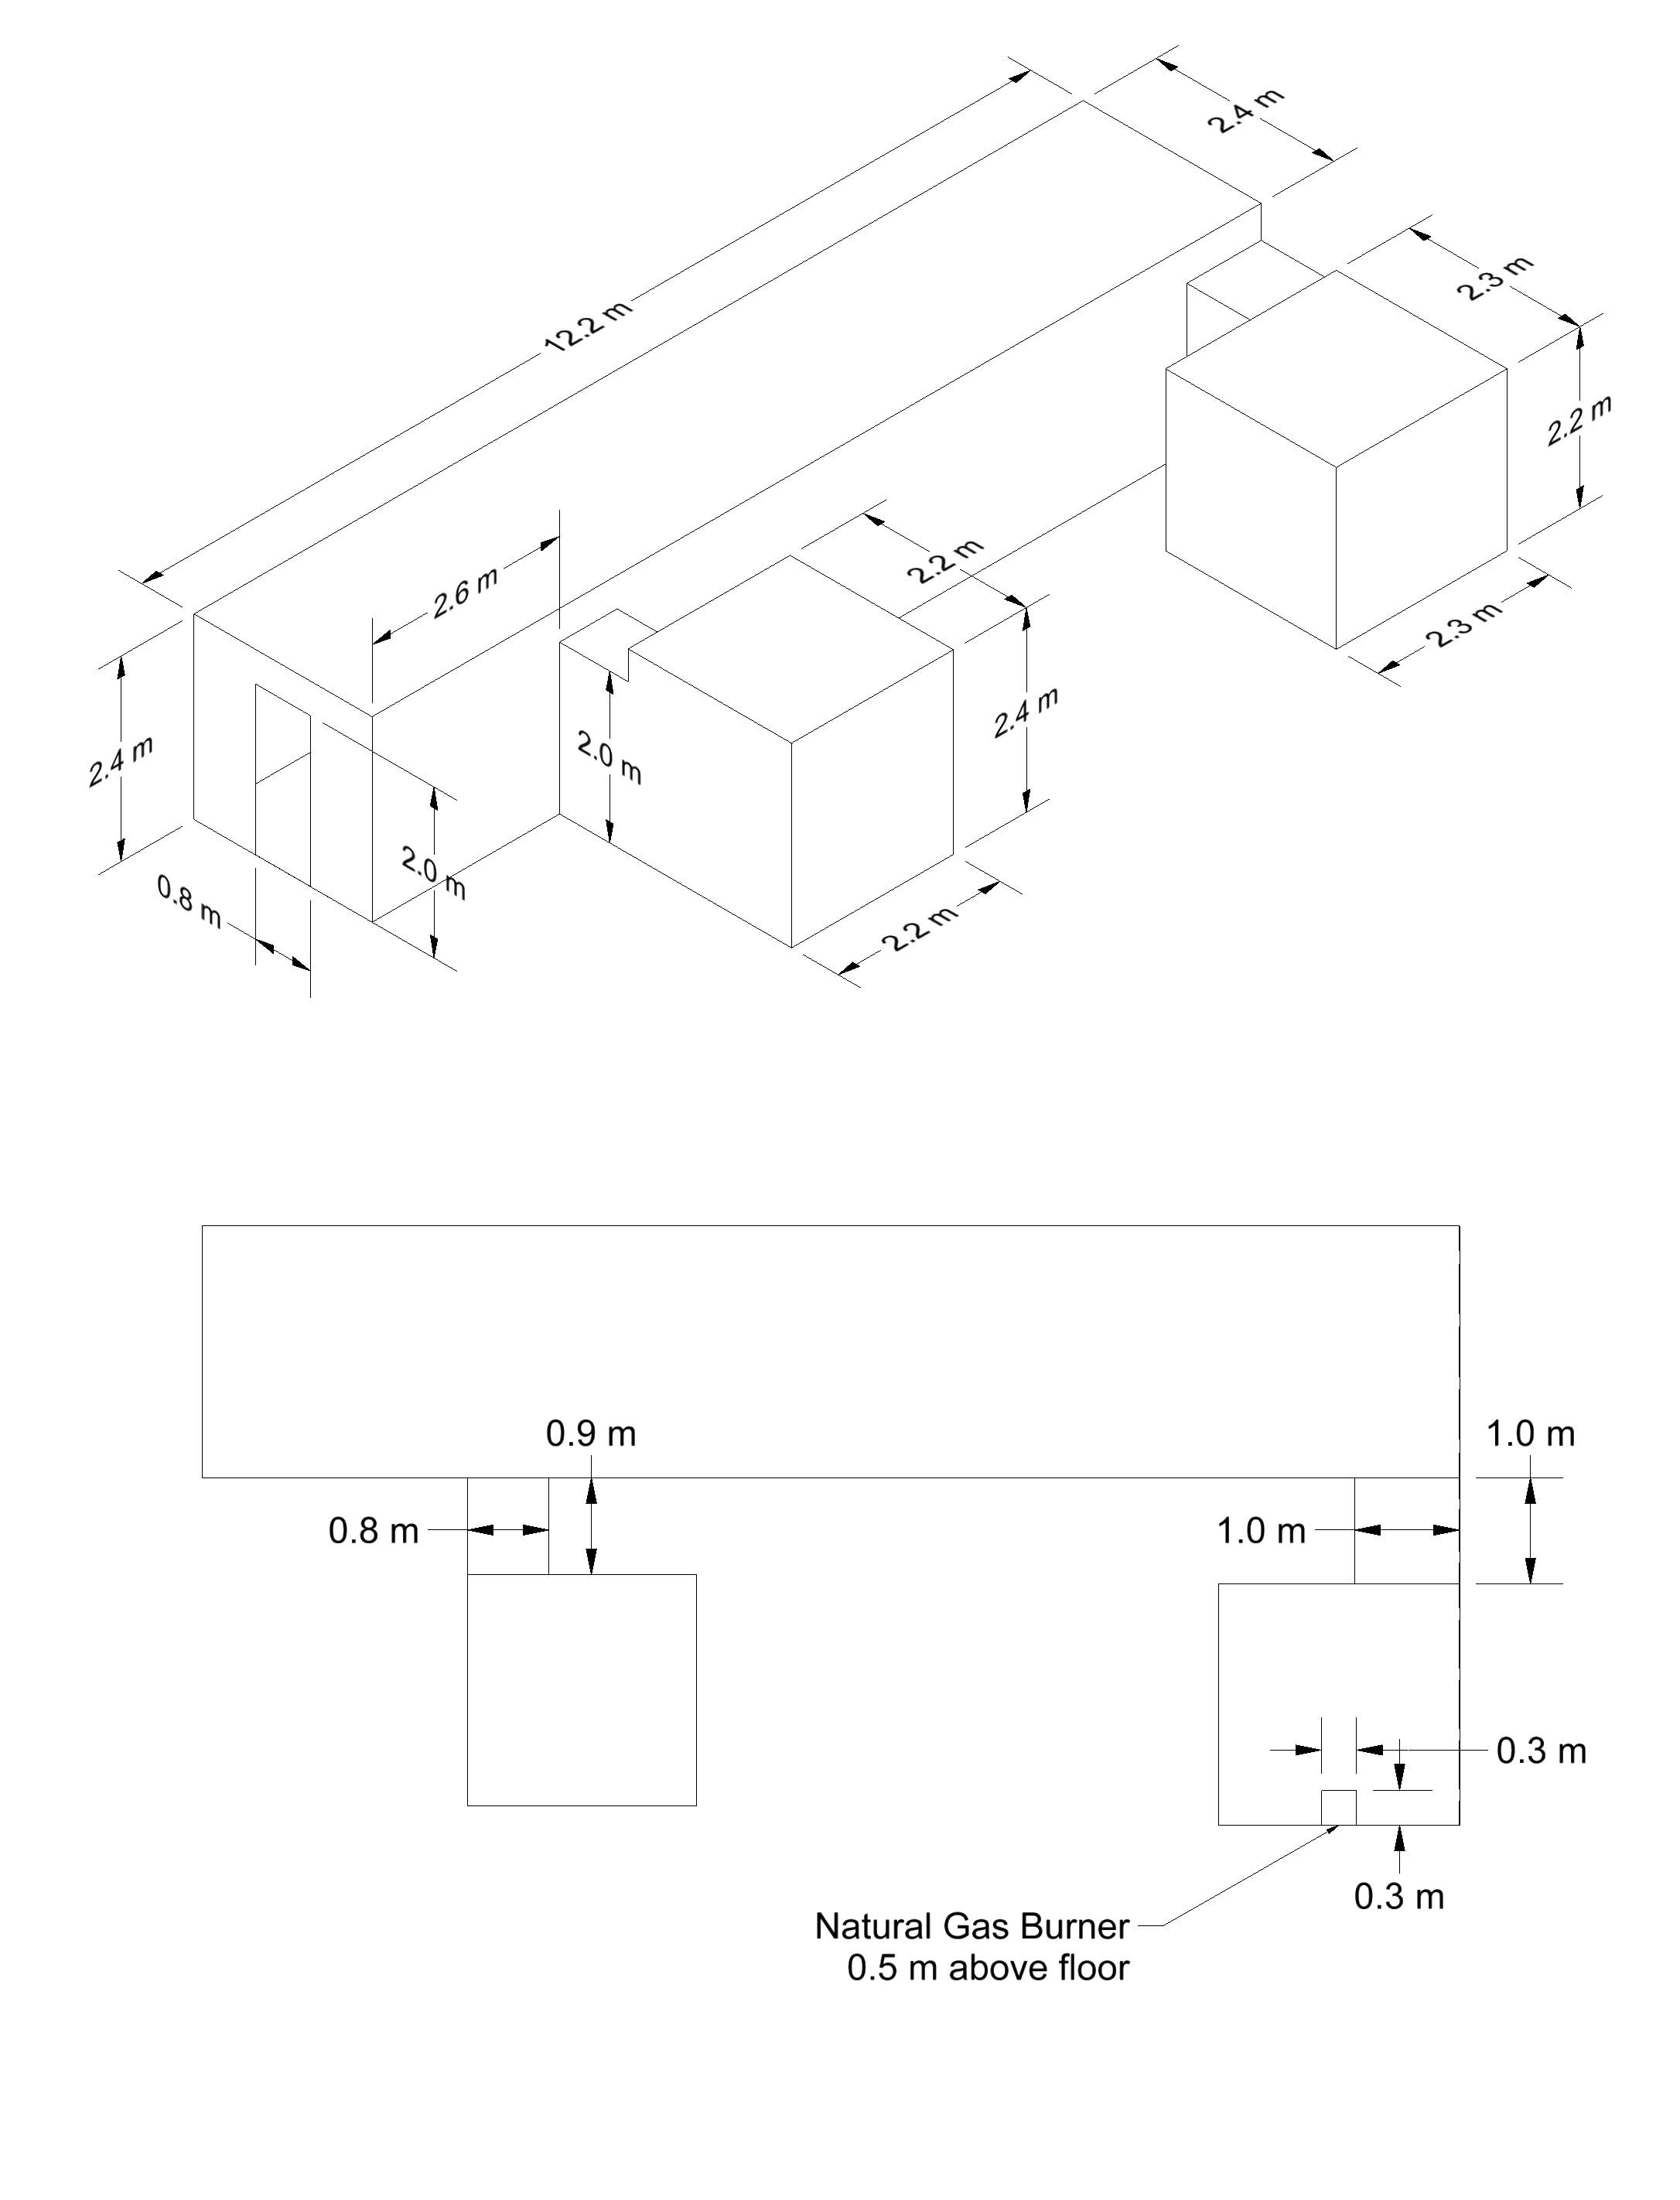
\includegraphics[width=6.5in]{FIGURES/NBS/NBS_Drawing}\\
\end{center}
\caption{Plan, side and perspective schematic drawings of the NBS experimental arrangement, including the burner.}
 \label{fig:NBS_Detailed}
\end{figure}

Figures \ref{fig:NBS_HRR} show the experimentally measured $\dQ$ as a function of time during Tests 100A and 100Z, respectively, of the NBS multi-room test series, typically averaging about 100 kW.  In these two tests, for which the door was open, the $\dQ$ during the steady burning period measured via oxygen consumption calorimetry was about 110 kW $\pm$ 17 kW ($\pm$ 15 \%). The combined relative expanded (2$\sigma$) uncertainty in the calorimetric  $\dQ$ is assigned a value of $\pm$~15~\%, consistent with the replicate measurements made during the experimental series and the uncertainty typical of oxygen consumption calorimetry. This value is also consistent with the measurement variation evident in the figures.  It was assumed that the closed door test (Test 100O) had the same $\dQ$ as the open door tests~\cite{NRCNUREG1824}.

\begin{figure}[\figoptions{t}]
\begin{center}
\begin{tabular}{cc}
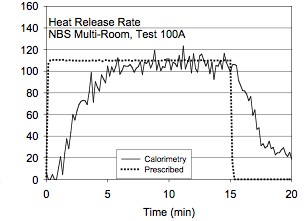
\includegraphics[width=3.0in]{FIGURES/NBS/NBS_HRR_100A} & 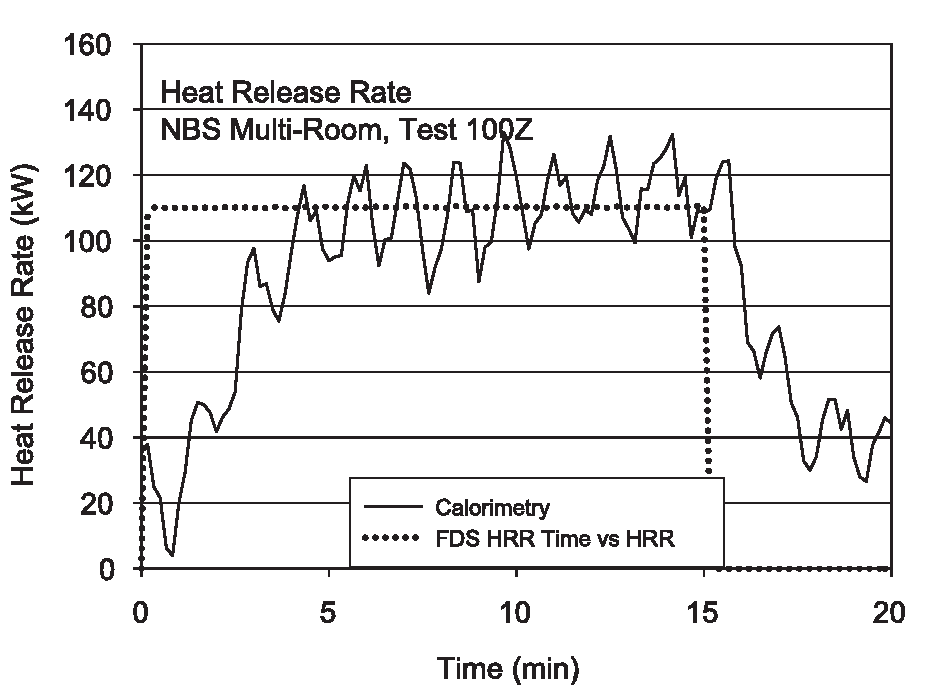
\includegraphics[width=3.0in]{FIGURES/NBS/NBS_HRR_100Z}\\
\end{tabular}
\end{center}
\caption{Prescribed and measured heat release rate as a function of time during Tests 100A and 100Z of the NBS multi-room test series.}
 \label{fig:NBS_HRR}
\end{figure}

The specified or prescribed  $\dQ$ is also shown in the figures.   The mass flow of the fuel (natural gas in Test 100A, or natural gas mixed with acetylene in Tests 100O and 100Z) was not metered; rather, the effluent was captured in a hood mounted above the open door in the corridor and the   was measured using oxygen consumption calorimetry.  The manner by which the fuel flow was controlled is not documented.  In Test 100A, candles were used to increase smoke in the upper layer to promote visualization. In Tests 100O and 100Z, acetylene was used (about 20 \% by volume) to produce smoke.  In those tests, the flow of natural gas and acetylene were adjusted to obtain approximately the same $\dQ$  as in Test 100A.  The addition of acetylene increased the radiative fraction of the fire.

For practical reasons, piped natural gas supplied by large utility companies is often used in fire experiments.  While its composition may vary from day to day, there is little change expected in the value of the radiative fraction \cite{NRCNUREG1824}. As mentioned above, natural gas was used as the fuel in Test 100A.  In Tests 100O and 100Z, acetylene was added to the natural gas to increase the smoke yield, and as a consequence, the radiative fraction increased.  The radiative fraction of natural gas has been studied previously, whereas the radiative fraction of the acetylene/natural gas mixture has not been studied. The radiative fraction for the natural gas fire was assigned a value of 0.20, whereas a value of 0.30 was assigned for the natural gas/acetylene fires \cite{NRCNUREG1824, Hamins:1991}.

The relative combined expanded (2$\sigma$) uncertainty in this parameter was assigned a value of $\pm$~20 \% in Test 100A and $\pm$~30 \% in 100O and 100Z.  The 20 \% expanded deviation value is consistent with typical values of the deviation reported in the literature for the measured radiative fraction.  The 100O and 100Z tests had a 50 \% larger value assigned, because the effect on the radiative fraction of adding acetylene to the natural gas was not measured~\cite{NRCNUREG1824}.

Measurements made during the NBS test series included gas and surface temperature, pressure, smoke and major gas species concentration, and doorway gas velocity.  Only two types of measurements conducted during the NBS test series were used in the evaluation considered here, because there was less confidence in the other measurements.  The measurements considered here were the HGL temperature and depth, in which bare bead thermocouples were used to make these measurements.  Single point measurements of temperature within the burn room were not used in the evaluation of plume or ceiling jet algorithms.  This is because, in neither instance, was the geometry consistent with the assumptions used in the model algorithms of plumes or jets. Specifically, the burner was mounted against a wall, and the room width to height ratio was less than that assumed by the various ceiling jet correlations.

\section{NIST Smoke Alarm Experiments}

A series of experiments was conducted by NIST to measure the activation time of ionization and photoelectric
smoke alarms in a residential setting~\cite{Bukowski:1}. Tests were conducted in actual homes with
representative sizes and floor plans, utilized actual furnishings and household items for fire sources,
and tested actual smoke alarms sold in retail stores at that time. Thirty-six tests were conducted in two
homes; 27 in a single-story manufactured home, and 8 in a two-story home.

Figure~\ref{NIST_Dunes_2000_Drawing} shows a diagram of the layout and instrumentation in the
manufactured home. The primary partitioning of the 84.7~m$^2$ floor plan consisted of three bedrooms:
one full bathroom, one kitchen/dining area, one living room, and two hallways. For testing, the doors
to bedroom 3 and the bathroom were always closed. The ceiling
was peaked on the long axis, reaching a height of 2.4~m. The outside walls
were approximately 2.1~m in height. The slope of the ceiling was approximately 8.4$^\circ$.

\begin{figure}
\begin{center}
\includegraphics[width=6.5in]{FIGURES/NIST_Dunes_2000/Manufactured_Home_Drawing}
\end{center}
\caption[Geometry of the NIST Dunes 2000 Experiments]{Geometry of the NIST Smoke Alarm Experiments.}
\label{NIST_Dunes_2000_Drawing}
\end{figure}

An upholstered chair, mattress, or pan of cooking oil was used as the fire source in each test.
There were three primary ignition sources: flaming, smoldering, and cooking.
The flaming ignition source used a moderate flame source to quickly ignite the fuel package.
Groups of smoke alarms were located in the room of fire origin, at least one bedroom, and
in a central location. Five stations (A-E) containing smoke alarm arrays were mounted parallel to the ceiling.

Nine experiments that were conducted in the single-story manufactured home were selected for model validation.
Only tests that used a flaming ignition source with a couch or mattress fuel package were considered;
the cooking oil fires and tests that used a smoldering ignition source were not considered.

Although a load cell was used in the experiments to measure the mass loss rate of the fuel package, the mass loss data
were not reliable enough to reconstruct the HRR curves for each test. Instead, the HRR curves were determined by approximating
the fire growth using a $t^2$ ramp, as in Eq.~(\ref{eq:t_squared}). The parameters for the $t^2$ ramp were calibrated in FDS
by using the temperature measured at the highest thermocouple in the tree (2~cm below the ceiling) in the fire room.
\be
\dot Q = \dot Q_0 \left( \frac{t}{\tau} \right)^2
\label{eq:t_squared}
\ee
A time offset was used to align the predicted ceiling thermocouple temperatures with the measured temperatures.
This offset is reported as the time at which the $t^2$ ramp begins.
The t-squared calibration parameters and time offsets for the HRR ramps are shown in Table~\ref{tab:NIST_Dunes_2000_Summary}.
Additionally, the ignition source had a small effect on the measured ceiling thermocouple temperatures. Therefore,
the size of the ignition source was approximated as either 3~kW or 7~kW, and the time offset of the ignition source was
also calibrated by using the measured ceiling thermocouple temperatures.
The resulting HRR curve was input into FDS as a fire ramp.

A summary of the nine tests selected for model validation is shown in Table~\ref{tab:NIST_Dunes_2000_Summary}.

\begin{table}[h!]
\caption{Summary of NIST Dunes 2000 experiments selected for model validation.}
\begin{center}
\begin{tabular}{|c|c|c|c|c|c|}
\hline
Test No.  &  Fire Source  &  Fire Location  &  $\dot Q_0$ (kW)  &  $\tau$ (s)  &  Time Offset (s)  \\ \hline \hline
SDC02     &  Chair        &  Living Room    &  150              &  180         &  20               \\ \hline
SDC05     &  Mattress     &  Bedroom        &  200              &  180         &  20               \\ \hline
SDC07     &  Mattress     &  Bedroom        &  350              &  180         &  50               \\ \hline
SDC10     &  Chair        &  Living Room    &  150              &  180         &  40               \\ \hline
SDC15     &  Chair        &  Living Room    &  225              &  400         &  180              \\ \hline
SDC33     &  Chair        &  Living Room    &  100              &  180         &  10               \\ \hline
SDC35     &  Chair        &  Living Room    &  100              &  180         &  10               \\ \hline
SDC38     &  Mattress     &  Bedroom        &  120              &  180         &  25               \\ \hline
SDC39     &  Mattress     &  Bedroom        &  200              &  180         &  25               \\ \hline
\end{tabular}
\end{center}
\label{tab:NIST_Dunes_2000_Summary}
\end{table}


%\section {NIST Seven-story Hotel Tests}

%By far the most complex test, this data set is part of  a series of full-scale experiments conducted to evaluate zoned smoke control systems, with and without stairwell pressurization cite{Klote:1990}.  It was conducted in a seven story hotel with multiple rooms on each floor and a stairwell connecting all floors.  This data set was chosen because it would challenge the scope of most current fire models.  Measured temperatures and pressure differences between the rooms and floors of the building are extensive and consistent.  Peak fire size was 3 MW with a total building volume of 140~000 m$^3$.

%Smoke movement and the performance of smoke control systems were studied in a seven story hotel building with smoke generated from wood fires and theatrical smoke. A total of 12 single experiments were conducted under a variety of conditions: two different fire sizes; sprinklered vs non-sprinklered wood fires; zoned smoke control on or off; stairwell pressurization on or off; with and without ventilation to the outside; and open and closed doors.

%The Plaza Hotel building was a masonry structure consisting of two wings, one three stories and the other seven stories tall. The two wings were built at different times. The wings were connected to each other at only one location on each floor. The connections between the wings at each floor were sealed off, and the fires were set on the second floor of the seven-story wing, using the shorter wing as an instrumentation area. Areas of the second floor were fire hardened to minimize structural damage to the building.

%\begin{figure}[\figoptions{t}]
%\begin{center}
%\begin{tabular}{cc}
%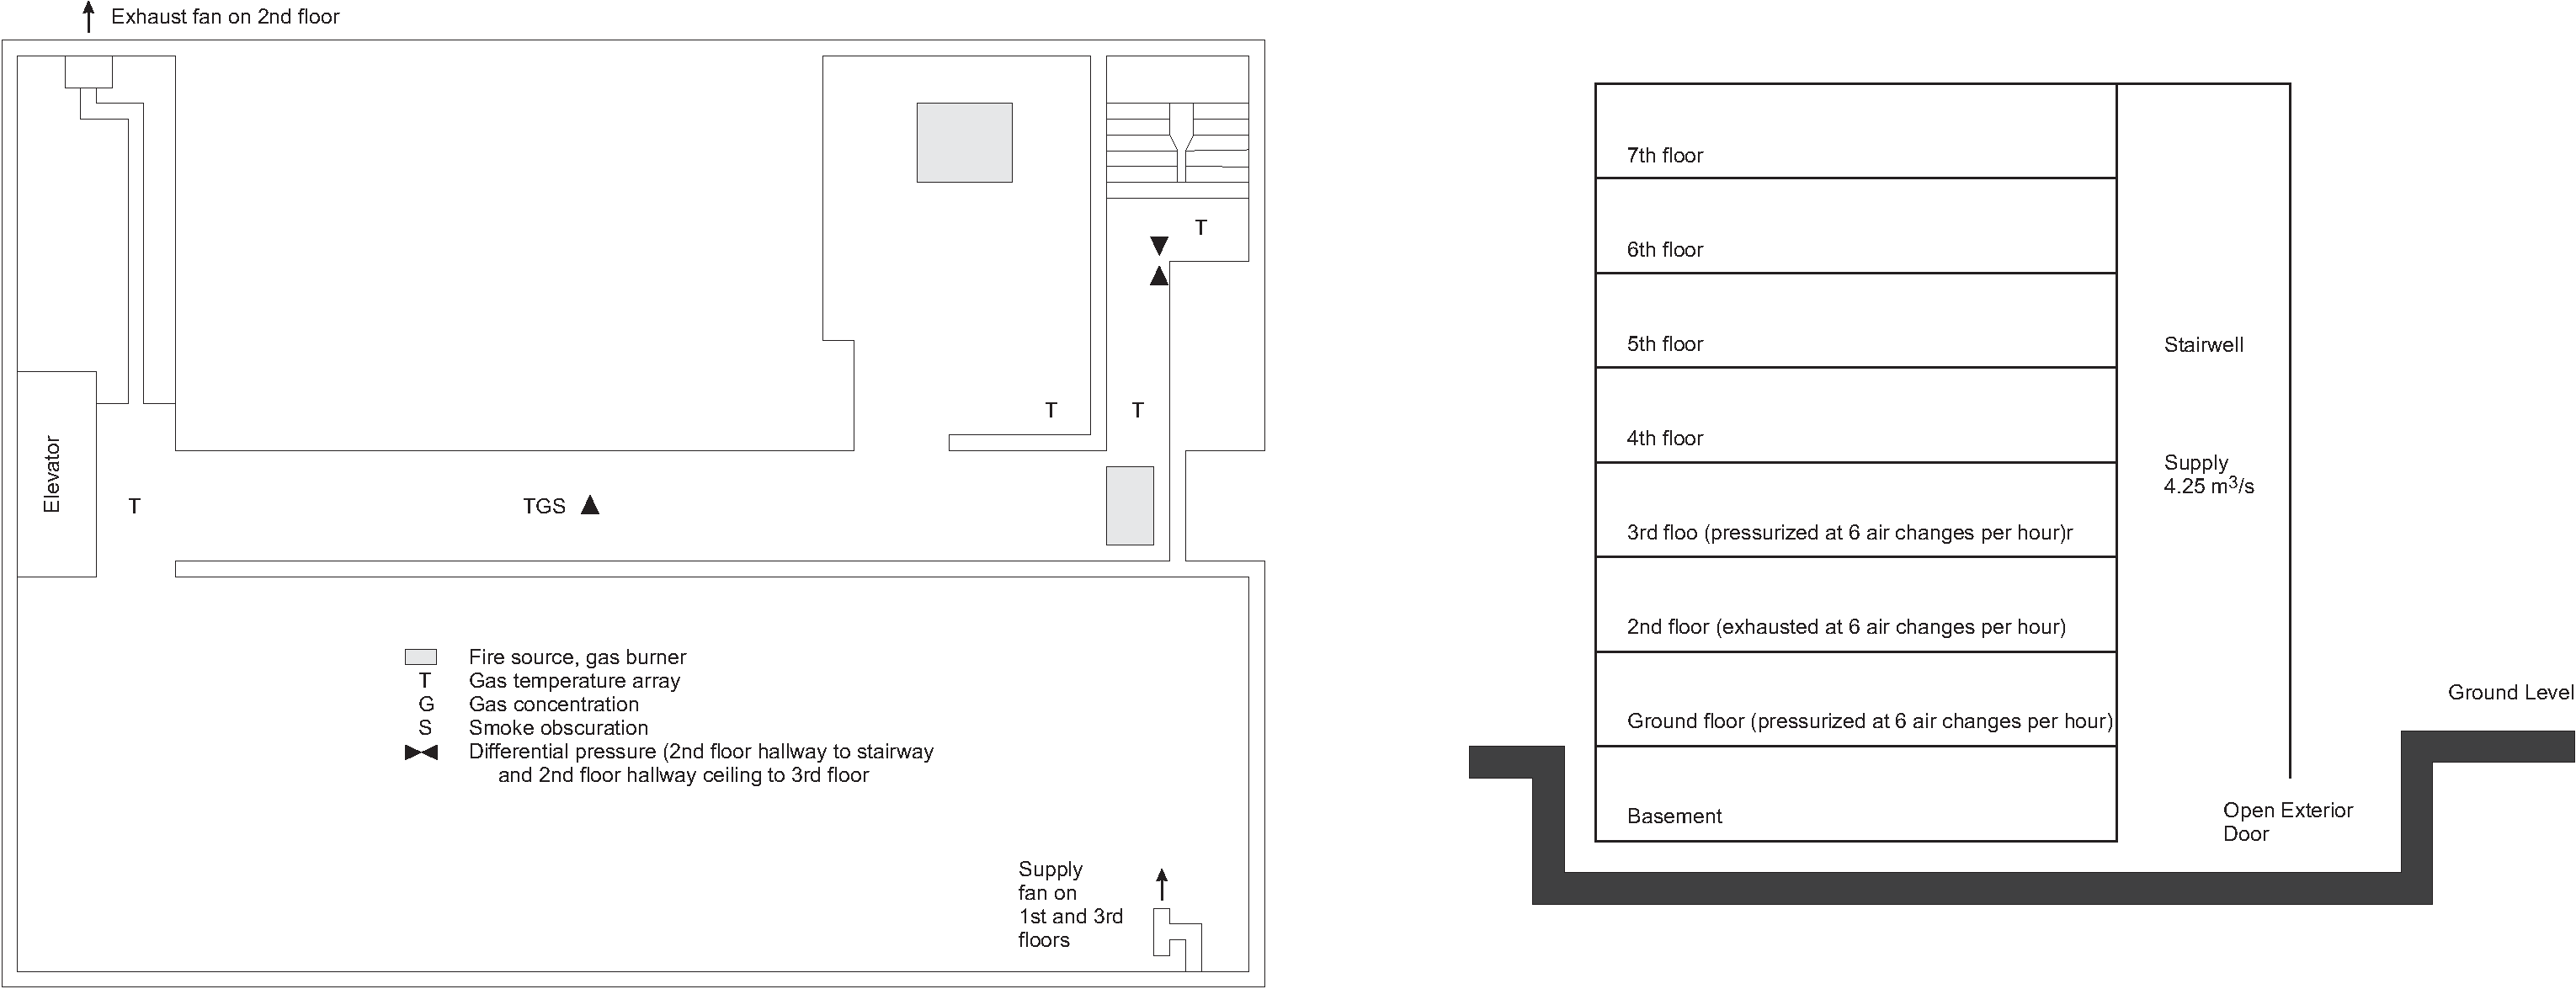
\includegraphics[width=6.0in]{FIGURES/NIST_PLAZA/PlazaSummary}\\
%\end{tabular}
%\end{center}
%\caption{Overview of the NIST Seven-story hotel test series including smoke control.}
% \label{fig:PlazaSummary}
%\end{figure}

%The smoke control systems were designed using the methods presented in the smoke control manual of the American Society of Heating, Refrigerating, and Air-Conditioning Engineers \cite{Klote:1983}, and the design analysis is discussed in detail by Klote \cite{Klote:1988}. The minimum design pressure difference was 25 Pa, meaning that the system should be able to maintain at least this value without a fire. The Plaza Hotel building had no central forced air heating, ventilating, and air-conditioning (HVAC) system, so a dedicated system of fans and ducts was installed for zoned smoke control and stairwell pressurization. The smoke control system consisted of the three 0.944 m$^3$/s centrifugal fans shown in \ref{fig:PlazaSummary}, plus another centrifugal fan (not shown) located outside and supplying 4.25 m$^3$/s of pressurization air to the stairwell at the first floor. The smoke control system is illustrated in figure \ref{fig:PlazaSummary}. All the test fires were located in the second floor smoke zone. This smoke was exhausted at about six air changes per hour. The first and second floors were pressurized at about six air changes per hour. When the stairwell pressurization system was activated, the exterior stairwell door was open. This approach is intended to minimize fluctuations due to opening and closing doors.

\section{NIST / NRC Test Series}

These experiments, sponsored by the US NRC and conducted at NIST, consisted of 15 large-scale experiments performed in June 2003. All 15 tests were included in the validation study. The experiments are documented in Ref.~\cite{Hamins:2005}. The fire sizes ranged from 350 kW to 2.2 MW in a compartment with dimensions 21.7~m by 7.1~m by 3.8~m high, designed to represent a compartment in a nuclear power plant containing power and control cables. A photo of the fire seen through the compartment doorway is shown in figure \ref{fig:NISTNRC_1MW_fire}. Figure \ref{fig:NISTNRC_Summary} shows the important features of the test hall. Figure \ref{fig:NISTNRC_Detailed} shows detailed plan, side and perspective schematic diagrams of the experimental arrangement. The walls and ceiling were covered with two layers of marinate boards, each layer 0.0125~m thick. The floor was covered with one layer of gypsum board on top of a layer of plywood. Thermophysical and optical properties of the marinate and other materials used in the compartment are given in reference \cite{Hamins:2005}. The room had one door and a mechanical air injection and extraction system. Ventilation conditions, the fire size, and fire location were varied. Numerous measurements (approximately 350 per test) were made including gas and surface temperatures, heat fluxes and gas velocities. Detailed schematic diagrams of the experimental arrangement are shown in figure \ref{fig:NISTNRC_Detailed}. Table \ref{tab:NISTNRC_Matrix} shows the experimental conditions for all 15 tests.

\begin{figure}[\figoptions{t}]
\begin{center}
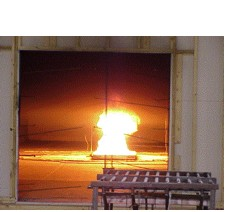
\includegraphics[width=4.0in]{FIGURES/NIST_NRC/NISTNRC_1MW_fire}\\
\end{center}
\caption{Photograph of a 1 MW heptane fire seen through the open doorway. Photo provided by Anthony Hamins, NIST.}
 \label{fig:NISTNRC_1MW_fire}
\end{figure}

\begin{figure}[\figoptions{t}]
\begin{center}
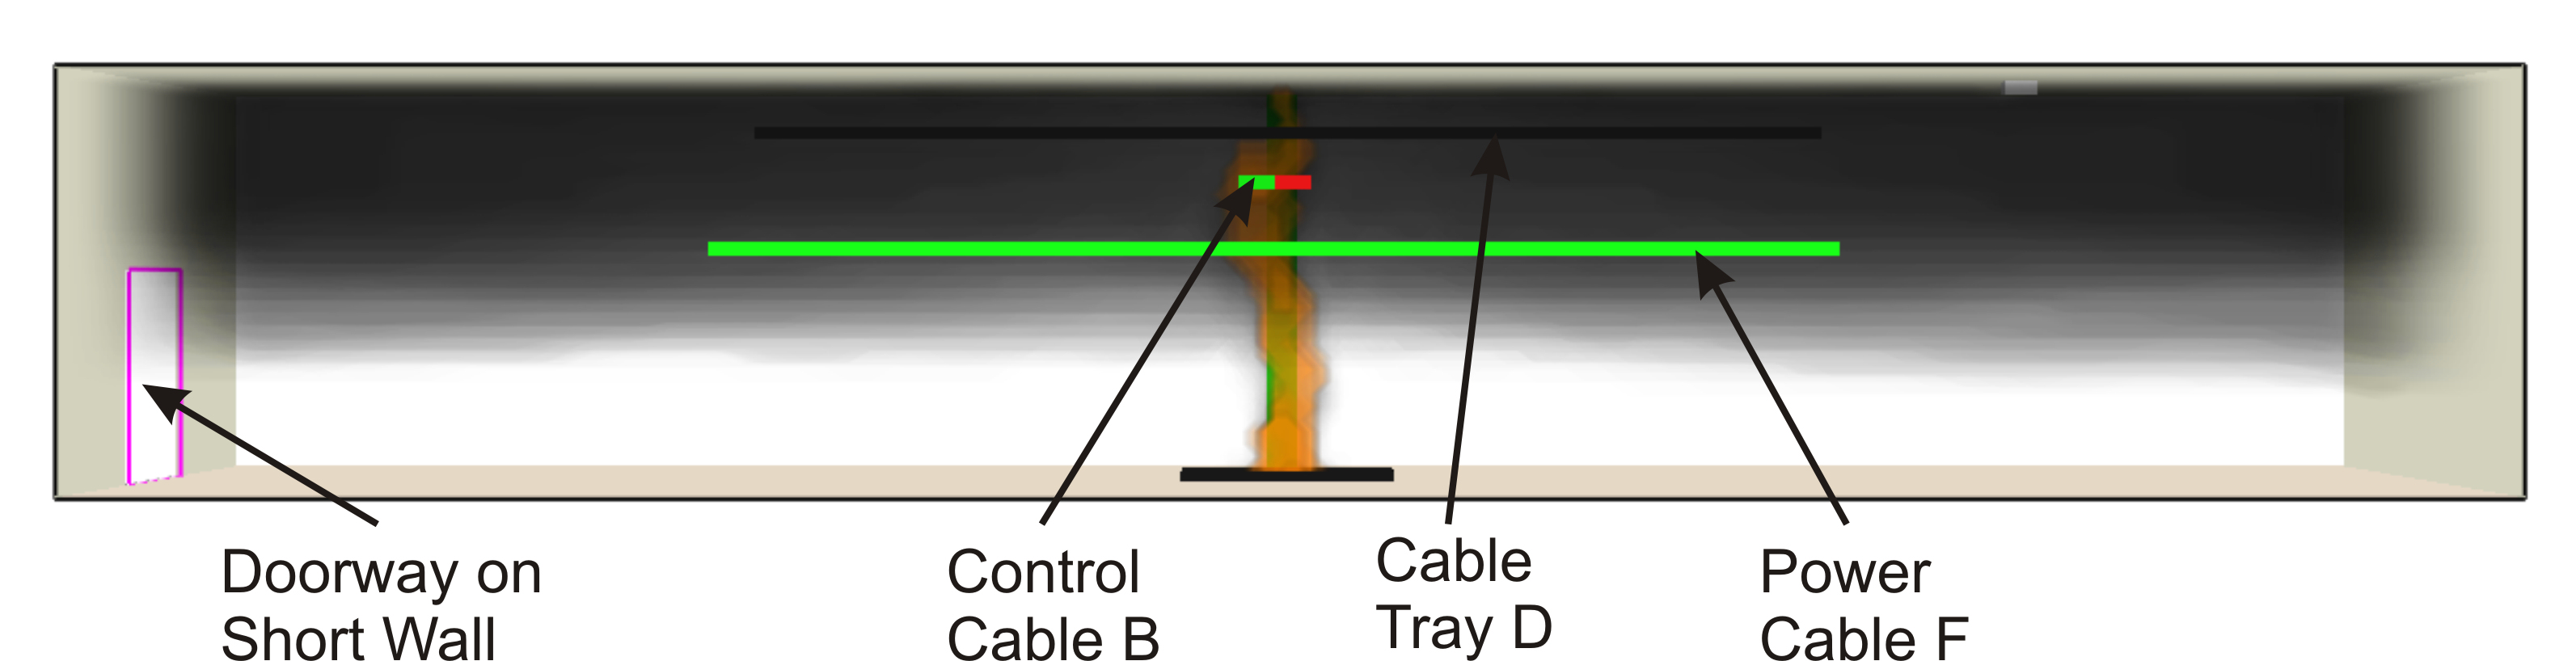
\includegraphics[width=5.0in]{FIGURES/NIST_NRC/NISTNRC_Summary}\\
\end{center}
\caption{Cross-section View of the NIST NRC Test Configuration.}
 \label{fig:NISTNRC_Summary}
\end{figure}

\begin{figure}[\figoptions{t}]
\begin{center}
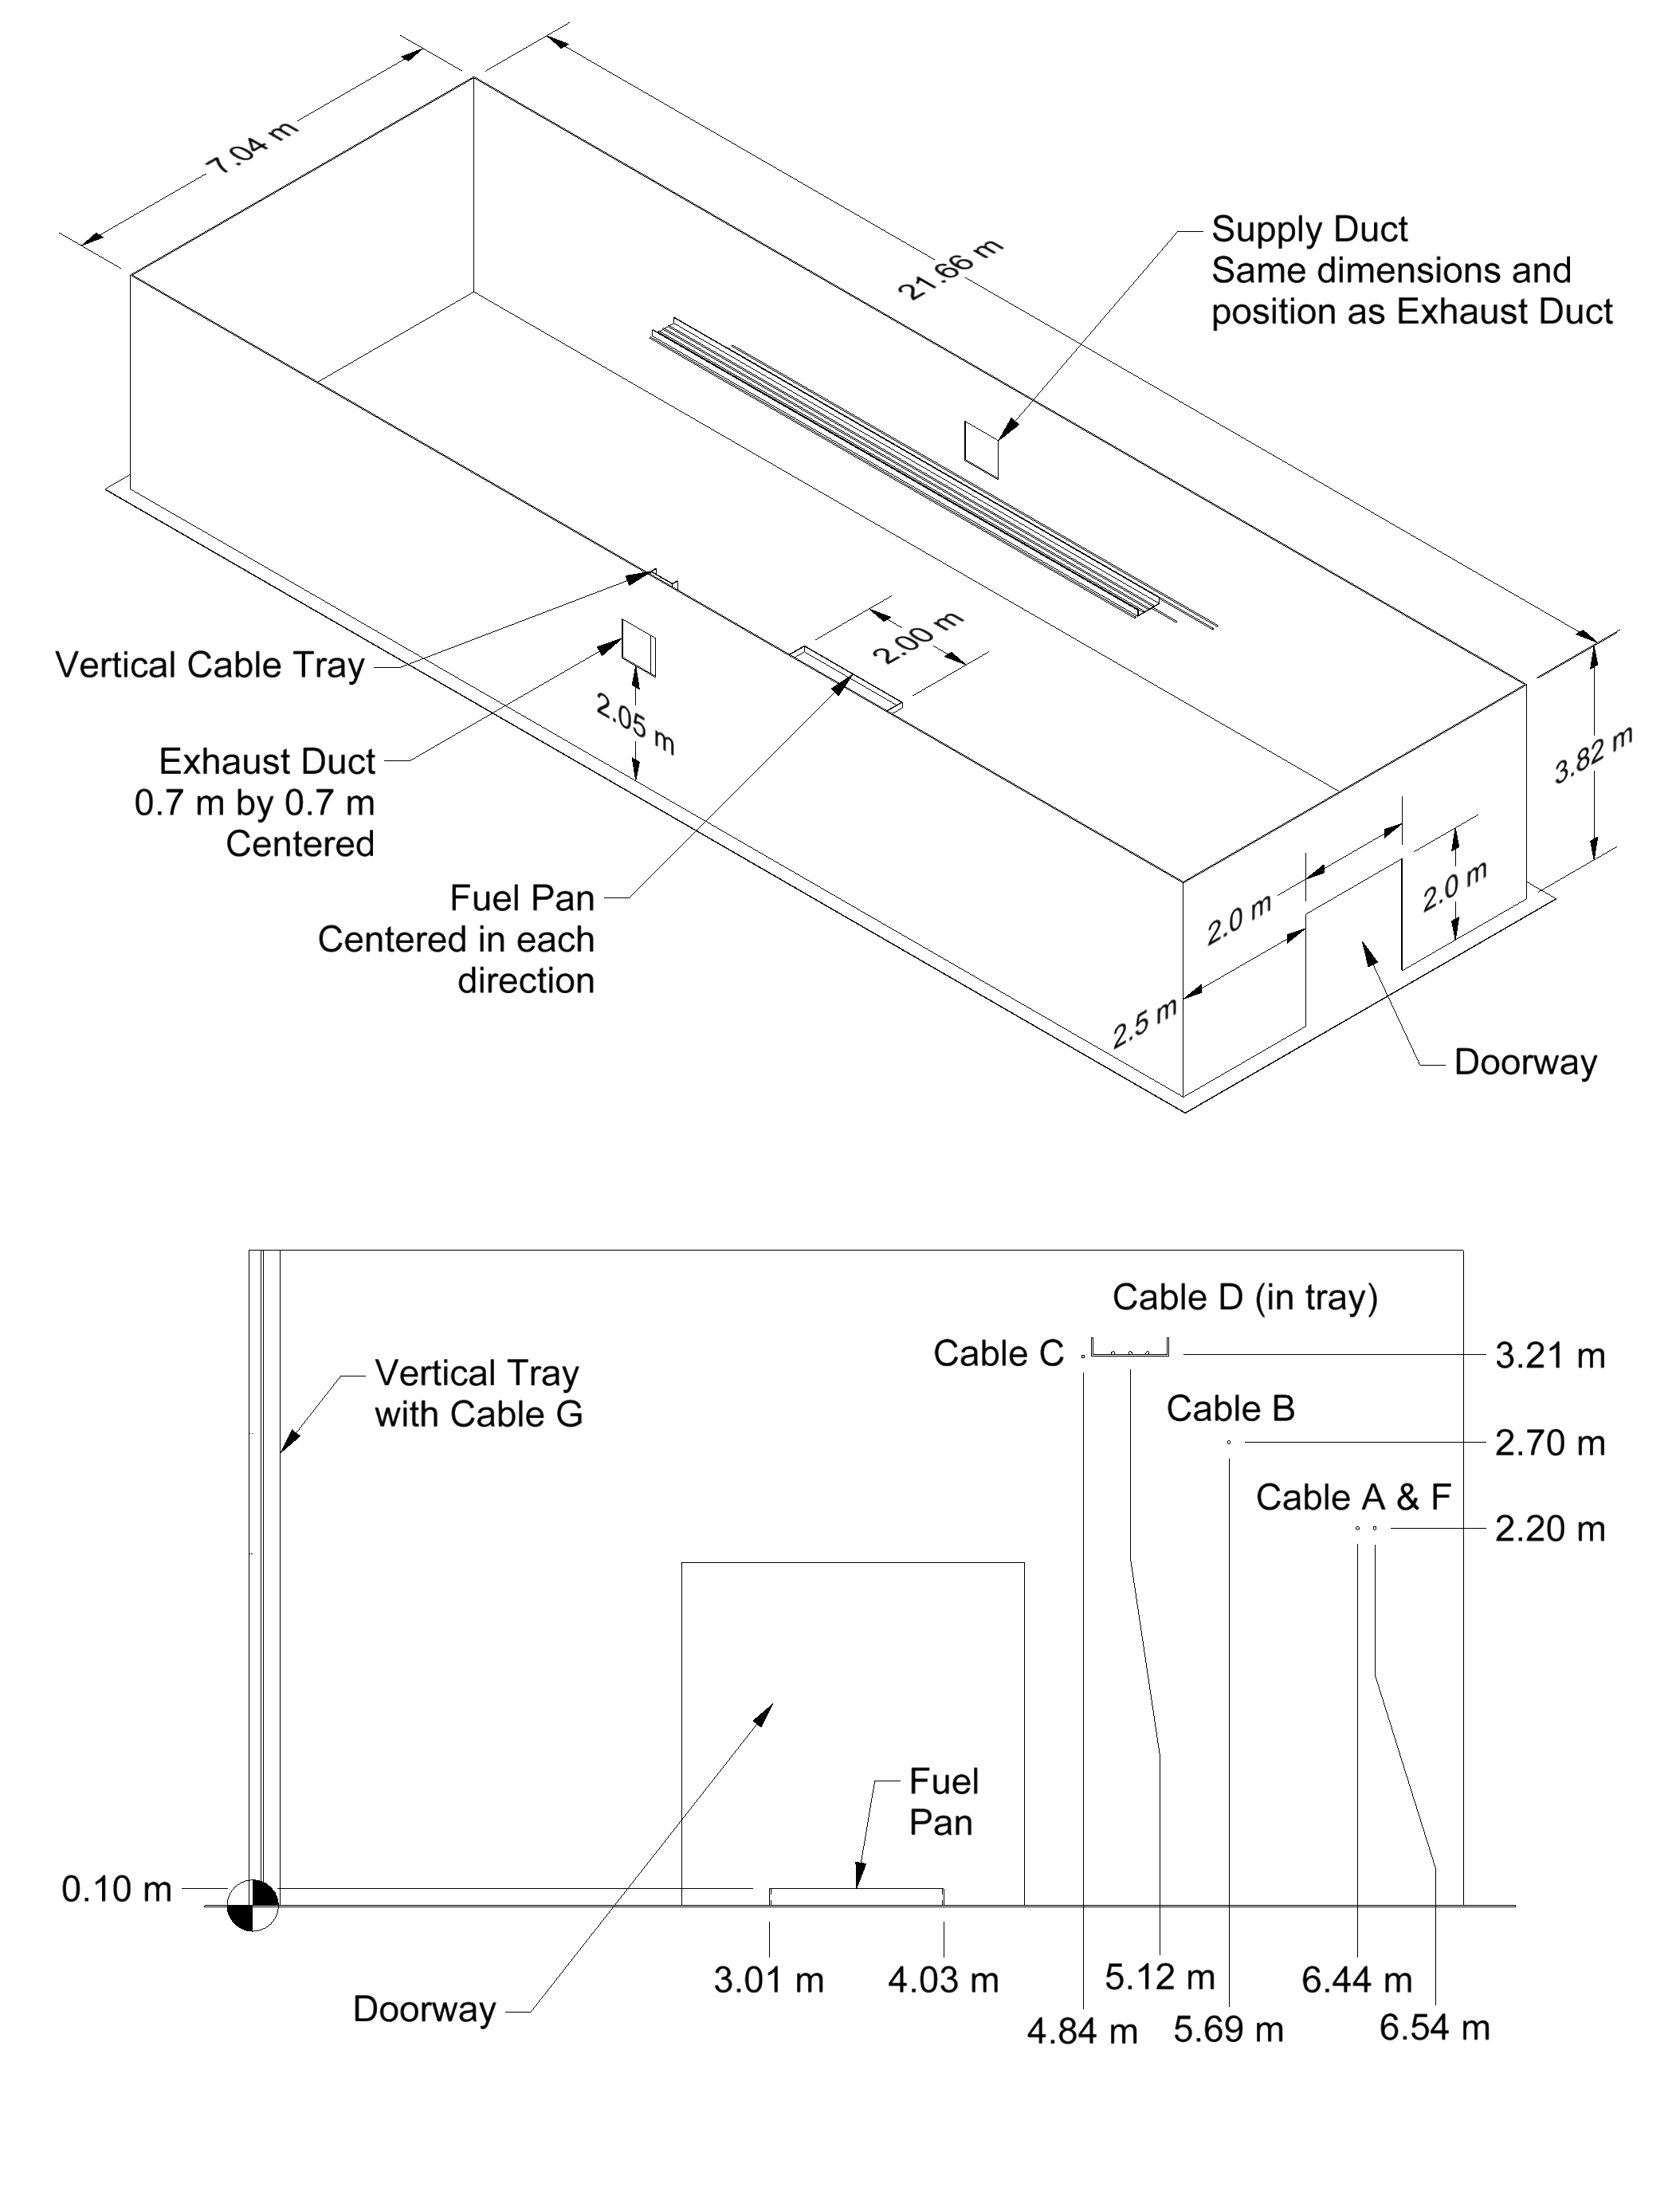
\includegraphics[width=6.5in]{FIGURES/NIST_NRC/NIST_NRC_Drawing}\\
\end{center}
\caption{Plan, side and perspective schematic drawings of the NIST NRC experimental arrangement. The fuel pan and cables B, D, F, and G (dotted lines) are also shown.}
 \label{fig:NISTNRC_Detailed}
\end{figure}

\begin{table}
\begin{center}
\caption{Test Matrix and Experimental Conditions for NIST NRC Tests}
\label{tab:NISTNRC_Matrix}
\vspace{0.1in}
\begin{tabular}{|c|c|c|c|c|c|}
\hline
Test & Nominal Peak & Cable & Fuel; Burner Location & Door & Mechanical\\
 & $\dQ$ (MW) & Type &  &  & Ventilation \\ \hline
\hline
1 & 0.35 & XPE\superscript{a} & Heptane; Center & Closed & Off \\ \hline
2 & 1 & XPE & Heptane; Center & Closed & Off \\ \hline
3 & 1 & XPE & Heptane; Center & Open & Off \\ \hline
4 & 1 & XPE & Heptane; Center & Closed & On \\ \hline
5 & 1 & XPE & Heptane; Center & Open & On \\ \hline
6 & \multicolumn{5}{|c|}{Not Conducted} \\ \hline
7 & 0.35 & PVC\superscript{b} & Heptane; Center & Closed & Off \\ \hline
8 & 1 & XPE & Heptane; Center & Closed & Off \\ \hline
9 & 1 & XPE & Heptane; Center & Open & Off \\ \hline
10 & 1 & PVC & Heptane; Center & Closed & On \\ \hline
11& \multicolumn{5}{|c|}{Not Conducted} \\ \hline
12 & \multicolumn{5}{|c|}{Not Conducted} \\ \hline
13 & 2 & XPE & Heptane; Center & Closed & Off \\ \hline
14 & 1 & XPE & Heptane; 1.8 m from N wall & Open & Off \\
 & & & on E-W centerline & & \\ \hline
15 & 1 & PVC & Heptane; 1.25 m from S wall & Open & Off \\
 & & & on E-W centerline & & \\ \hline
 16 & 2 & PVC & Heptane; Center & Closed & On \\ \hline
 17 & 1 & PVC & Toluene; Center & Closed & Off \\ \hline
18 & 1 & XPE & Heptane; 1.55 m from S wall & Open & Off \\
 & & & 1.50 m E of centerline & & \\ \hline
\multicolumn{6}{l}{a - XPE cable has crosslinked polyethylene jacket insulation} \\
\multicolumn{6}{l}{b - PVC cable has a polyvinylchloride jacket insulation}
\end{tabular}
\end{center}
\end{table}

The compartment had a 2 m by 2 m door in the middle of the west wall. Some of the tests had a closed door and no mechanical ventilation, and in those tests the measured compartment leakage was an important consideration. Reference \cite{Hamins:2005} reports leakage area based on measurements performed periodically during the test series. For the closed door tests, the leakage area used in the simulations was based on the last available measurement. It should be noted that the chronological order of the tests differed from the numerical order \cite{Hamins:2005}.

The mechanical ventilation and exhaust was used during some test, providing about 5 air changes per hour. The supply duct was positioned on the long wall, about 2 m off the floor. An exhaust duct of equal area to the supply duct was positioned on the opposite wall at a comparable location. The flow rates through the supply and exhaust ducts were measured in detail during breaks in the testing, in the absence of a fire. During the tests, the flows were monitored with single bi-directional probes during the tests themselves.

A single nozzle was used to spray liquid hydrocarbon fuels onto a 1 m by 2 m fire pan that was about 0.02 m deep. The test plan originally called for the use of two nozzles to provide the fuel spray. Experimental observation suggested that the fire was more steady with the use of a single nozzle. In addition, it was observed that the actual extent of the liquid pool was well-approximated by a 1 m circle in the center of the pan. For safety reasons, the fuel flow was terminated when the lower-layer oxygen concentration dropped to approximately 15~\% by volume. The fuel used in 14 of the tests was heptane, while toluene was used for one test. The HRR was determined using oxygen consumption calorimetry (figure \ref{fig:NISTNRC_HRR} shows a sample heat release rate for one of the tests in the series). The recommended uncertainty values for HRR were 17~\% for all of the tests. The radiative fraction was measured in an independent study for the same fuels using the same spray burner as used in the test series \cite{Hamins:2003}. The value of the radiative fraction and its uncertainty were reported as 0.44 $\pm$ 16 \% and 0.40 $\pm$ 23 \% for heptane and toluene, respectively. Further details of the model inputs used for these simulations are included in reference \cite{NRCNUREG1824}.

\begin{figure}[\figoptions{t}]
\begin{center}
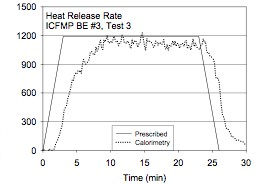
\includegraphics[width=3.0in]{FIGURES/NIST_NRC/NISTNRC_HRR}\\
\end{center}
\caption{Measured and prescribed heat release rate as a function of time during Test 3 of the NIST NRC test series}
 \label{fig:NISTNRC_HRR}
\end{figure}

\section{SP Adiabatic Surface Temperature Experiments}

In 2008, three compartment experiments were performed at SP Technical Research Institute of Sweden under the sponsorship of Brandforsk, the Swedish Fire Research Board~\cite{Wickstrom_AST}. The objective of the experiments was to demonstrate how plate thermometer measurements in the vicinity of a simple steel beam can be used to supply the boundary conditions for a multi-dimensional heat conduction calculation for the beam. The adiabatic surface temperature was derived from the plate temperatures and used by TASEF, a finite-element
thermal-structural program.

The experiments were performed inside a standard compartment designed for corner fire testing (ISO 9705). The compartment is 3.6~m deep, 2.4~m wide and 2.4~m high and includes a door opening 0.8~m by 2.0~m. The room was constructed of 20~cm thick light weight concrete blocks with a density of 600~kg/m$^3$~$\pm$~100~kg/m$^3$. The heat source was a gas burner run at a constant power of 450~kW. The top of the burner, with a square opening 30~cm by 30~cm, was placed 65~cm above the floor, 2.5~cm from the walls. A single steel beam was suspended 20~cm below the ceiling along the centerline of the compartment. There were three measurement stations along the beam at lengths of 0.9~m (Position A), 1.8~m (Position B), and 2.7~m (Position C) from the far wall where the fire was either positioned in the corner (Tests 1 and 2), or the center (Test 3). The beam in Test 1 was a rectangular steel tube filled with an insulation material. The beam in Tests 2 and 3 was an I-beam.  A diagram of the room used in Test~2 is displayed in Figure~\ref{Room_Drawing}.

\begin{figure}[ht]
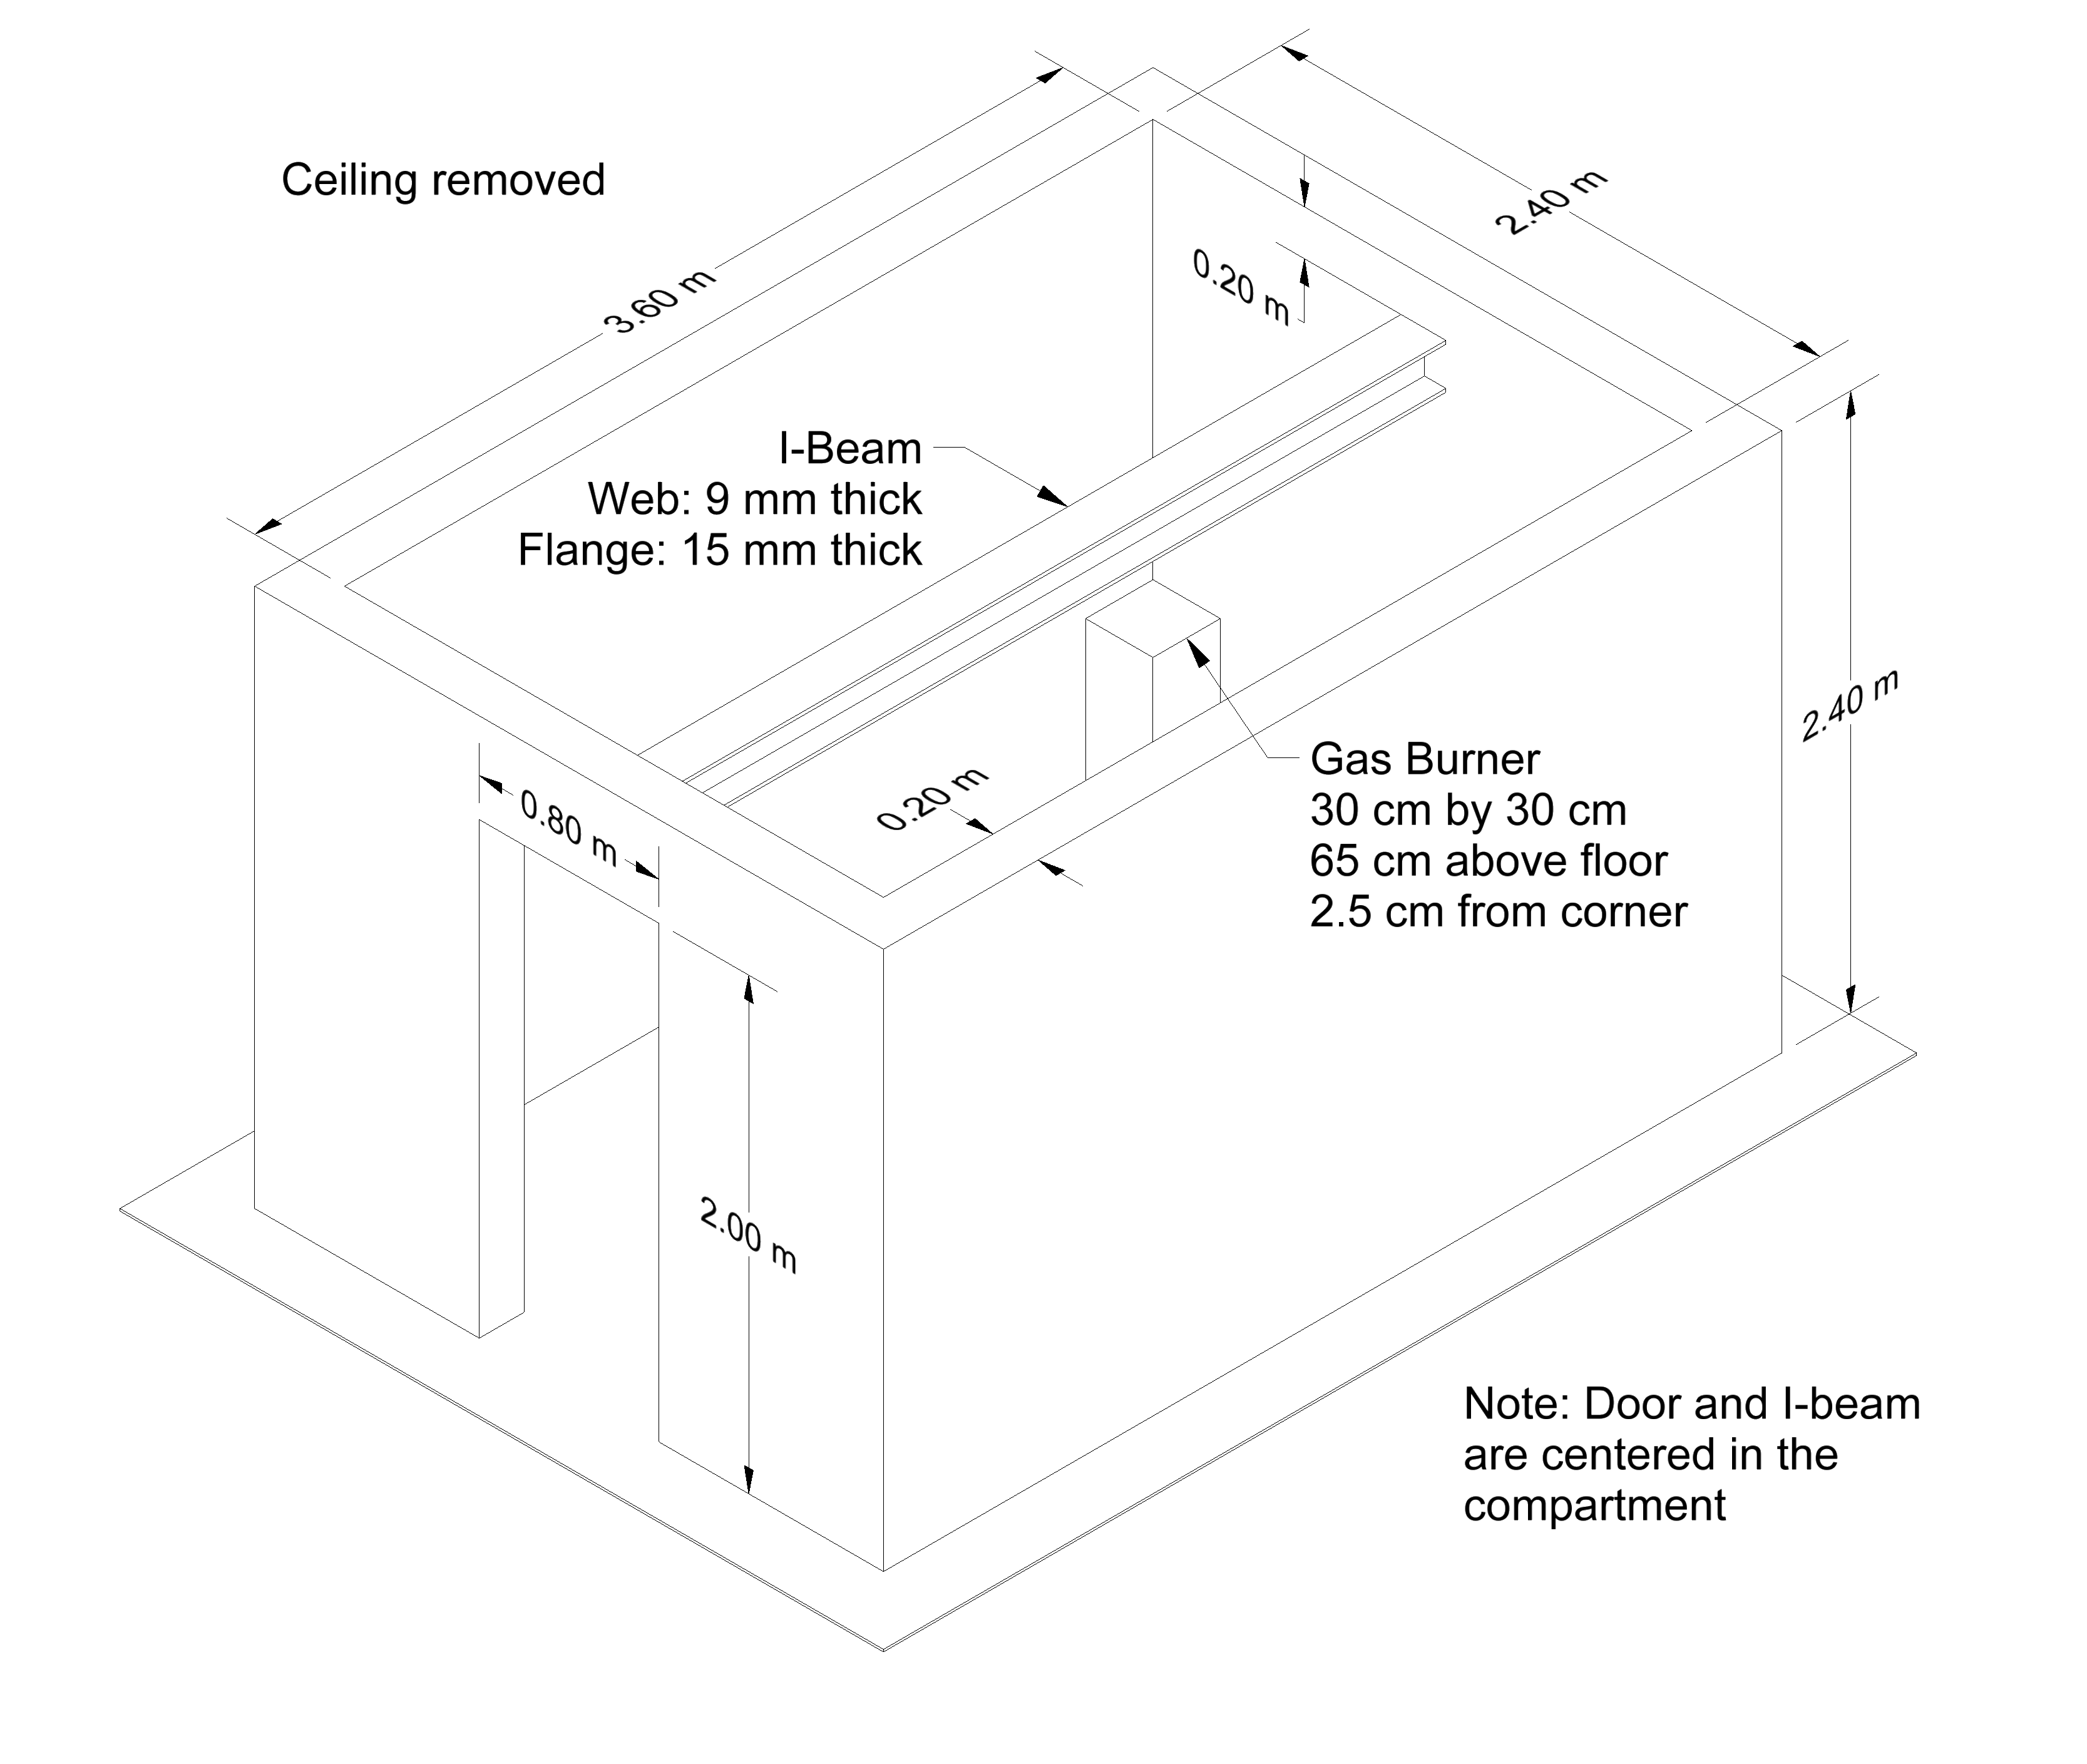
\includegraphics[width=\textwidth]{FIGURES/SP_AST/SP_AST_Compartment_Drawing.png}
\caption{Geometry of the  SP/AST compartment for Test 2.}
\label{Room_Drawing}
\end{figure}

A second series of experiments involving plate thermometers was carried out in 2011~\cite{Sjostrom:AST}. A 6~m long, 20~cm diameter vertical steel column was positioned in the center of 1.1~m and 1.9~m diesel fuel and 1.1~m heptane pool fires. Gas, plate thermometer, and surface temperatures were measured at heights of 1~m, 2~m, 3~m, 4~m, and 5~m above the pool surface. These experiments are notable because the column is partially engulfed in flames.

\section{Steckler Compartment Experiments}

Steckler, Quintiere and Rinkinen performed a set of 55 compartment fire tests at NBS in 1979 \cite{Steckler:1982}. The compartment was 2.8~m by 2.8~m by 2.13~m high\footnote{The test report
gives the height of the compartment as 2.18~m. This is a misprint. The compartment was 2.13~m high.}, with a single door of
various widths, or alternatively a single window with various heights. A 30~cm diameter methane burner was used to generate fires with heat release rates of
31.6~kW, 62.9~kW, 105.3~kW and 158~kW. Vertical profiles of velocity and temperature were measured in the doorway, along with a single vertical profile of temperature
within the compartment.
A full description and results are reported in Reference~ \cite{Steckler:1982}. The basic test matrix is listed in Table~\ref{Steckler_Table}. Note that the
test report does not include a detailed description of the compartment. However, an internal report\footnote{ {\em Technical Research Report, Fire Induced Flows
Through Room Openings - Flow Coefficients}, Project 203005-003, Armstrong Cork Company, Lancaster, Pennsylvania, May, 1981.} by the test sponsor, Armstrong Cork Company,
reports that the compartment floor was composed of 19~mm calcium silicate board on top of 12.7~mm plywood on wood joists. The walls and ceiling consisted of
12.7~mm ceramic fiber insulation board over 0.66~mm aluminum sheet attached to wood studs. A diagram of the compartment is displayed in Fig.~\ref{Steckler_ Drawing}.

\begin{table}
\caption{Summary of Steckler compartment experiments.}
\begin{center}
\begin{tabular}{|c|c|c|c|c||c|c|c|c|c|}
\hline
        & Opening   & Opening       &  HRR       & Burner       &       & Opening   & Opening     &  HRR         & Burner        \\
Test    & Width     & Height        & $\dot{Q}$  & Location     & Test  & Width     & Height      & $\dot{Q}$    & Location      \\
        & (m)       & (m)           & (kW)       &              &       & (m)       &  (m)        & (kW)         &                \\ \hline \hline
10      & 0.24      & 1.83          &  62.9      & Center       & 224   & 0.74      & 0.92        &  62.9         & Back Corner         \\ \hline
11      & 0.36      & 1.83          &  62.9      & Center       & 324   & 0.74      & 0.92        &  62.9         & Back Corner         \\ \hline
12      & 0.49      & 1.83          &  62.9      & Center       & 220   & 0.74      & 1.83        &  31.6         & Back Corner         \\ \hline
612     & 0.49      & 1.83          &  62.9      & Center       & 221   & 0.74      & 1.83        &  105.3        & Back Corner         \\ \hline
13      & 0.62      & 1.83          &  62.9      & Center       & 514   & 0.24      & 1.83        &  62.9         & Back Wall           \\ \hline
14      & 0.74      & 1.83          &  62.9      & Center       & 544   & 0.36      & 1.83        &  62.9         & Back Wall           \\ \hline
18      & 0.74      & 1.83          &  62.9      & Center       & 512   & 0.49      & 1.83        &  62.9         & Back Wall           \\ \hline
710     & 0.74      & 1.83          &  62.9      & Center       & 542   & 0.62      & 1.83        &  62.9         & Back Wall           \\ \hline
810     & 0.74      & 1.83          &  62.9      & Center       & 610   & 0.74      & 1.83        &  62.9         & Back Wall           \\ \hline
16      & 0.86      & 1.83          &  62.9      & Center       & 510   & 0.74      & 1.83        &  62.9         & Back Wall           \\ \hline
17      & 0.99      & 1.83          &  62.9      & Center       & 540   & 0.86      & 1.83        &  62.9         & Back Wall           \\ \hline
22      & 0.74      & 1.38          &  62.9      & Center       & 517   & 0.99      & 1.83        &  62.9         & Back Wall           \\ \hline
23      & 0.74      & 0.92          &  62.9      & Center       & 622   & 0.74      & 1.38        &  62.9         & Back Wall           \\ \hline
30      & 0.74      & 0.92          &  62.9      & Center       & 522   & 0.74      & 1.38        &  62.9         & Back Wall           \\ \hline
41      & 0.74      & 0.46          &  62.9      & Center       & 524   & 0.74      & 0.92        &  62.9         & Back Wall           \\ \hline
19      & 0.74      & 1.83          &  31.6      & Center       & 541   & 0.74      & 0.46        &  62.9         & Back Wall           \\ \hline
20      & 0.74      & 1.83          &  105.3     & Center       & 520   & 0.74      & 1.83        &  31.6         & Back Wall           \\ \hline
21      & 0.74      & 1.83          &  158.0     & Center       & 521   & 0.74      & 1.83        &  105.3        & Back Wall           \\ \hline
114     & 0.24      & 1.83          &  62.9      & Back Corner  & 513   & 0.74      & 1.83        &  158.0        & Back Wall           \\ \hline
144     & 0.36      & 1.83          &  62.9      & Back Corner  & 160   & 0.74      & 1.83        &  62.9         & Center$^*$          \\ \hline
212     & 0.49      & 1.83          &  62.9      & Back Corner  & 163   & 0.74      & 1.83        &  62.9         & Back Corner$^*$     \\ \hline
242     & 0.62      & 1.83          &  62.9      & Back Corner  & 164   & 0.74      & 1.83        &  62.9         & Back Wall$^*$       \\ \hline
410     & 0.74      & 1.83          &  62.9      & Back Corner  & 165   & 0.74      & 1.83        &  62.9         & Left Wall$^*$       \\ \hline
210     & 0.74      & 1.83          &  62.9      & Back Corner  & 162   & 0.74      & 1.83        &  62.9         & Right Wall$^*$      \\ \hline
310     & 0.74      & 1.83          &  62.9      & Back Corner  & 167   & 0.74      & 1.83        &  62.9         & Front Center$^*$    \\ \hline
240     & 0.86      & 1.83          &  62.9      & Back Corner  & 161   & 0.74      & 1.83        &  62.9         & Doorway$^*$         \\ \hline
116     & 0.99      & 1.83          &  62.9      & Back Corner  & 166   & 0.74      & 1.83        &  62.9         & Front Corner$^*$    \\ \hline
122     & 0.74      & 1.38          &  62.9      & Back Corner  &  \multicolumn{5}{r|}{$^*$ Raised burner}                   \\ \hline
\end{tabular}
\end{center}
\label{Steckler_Table}
\end{table}

\begin{figure}[p]
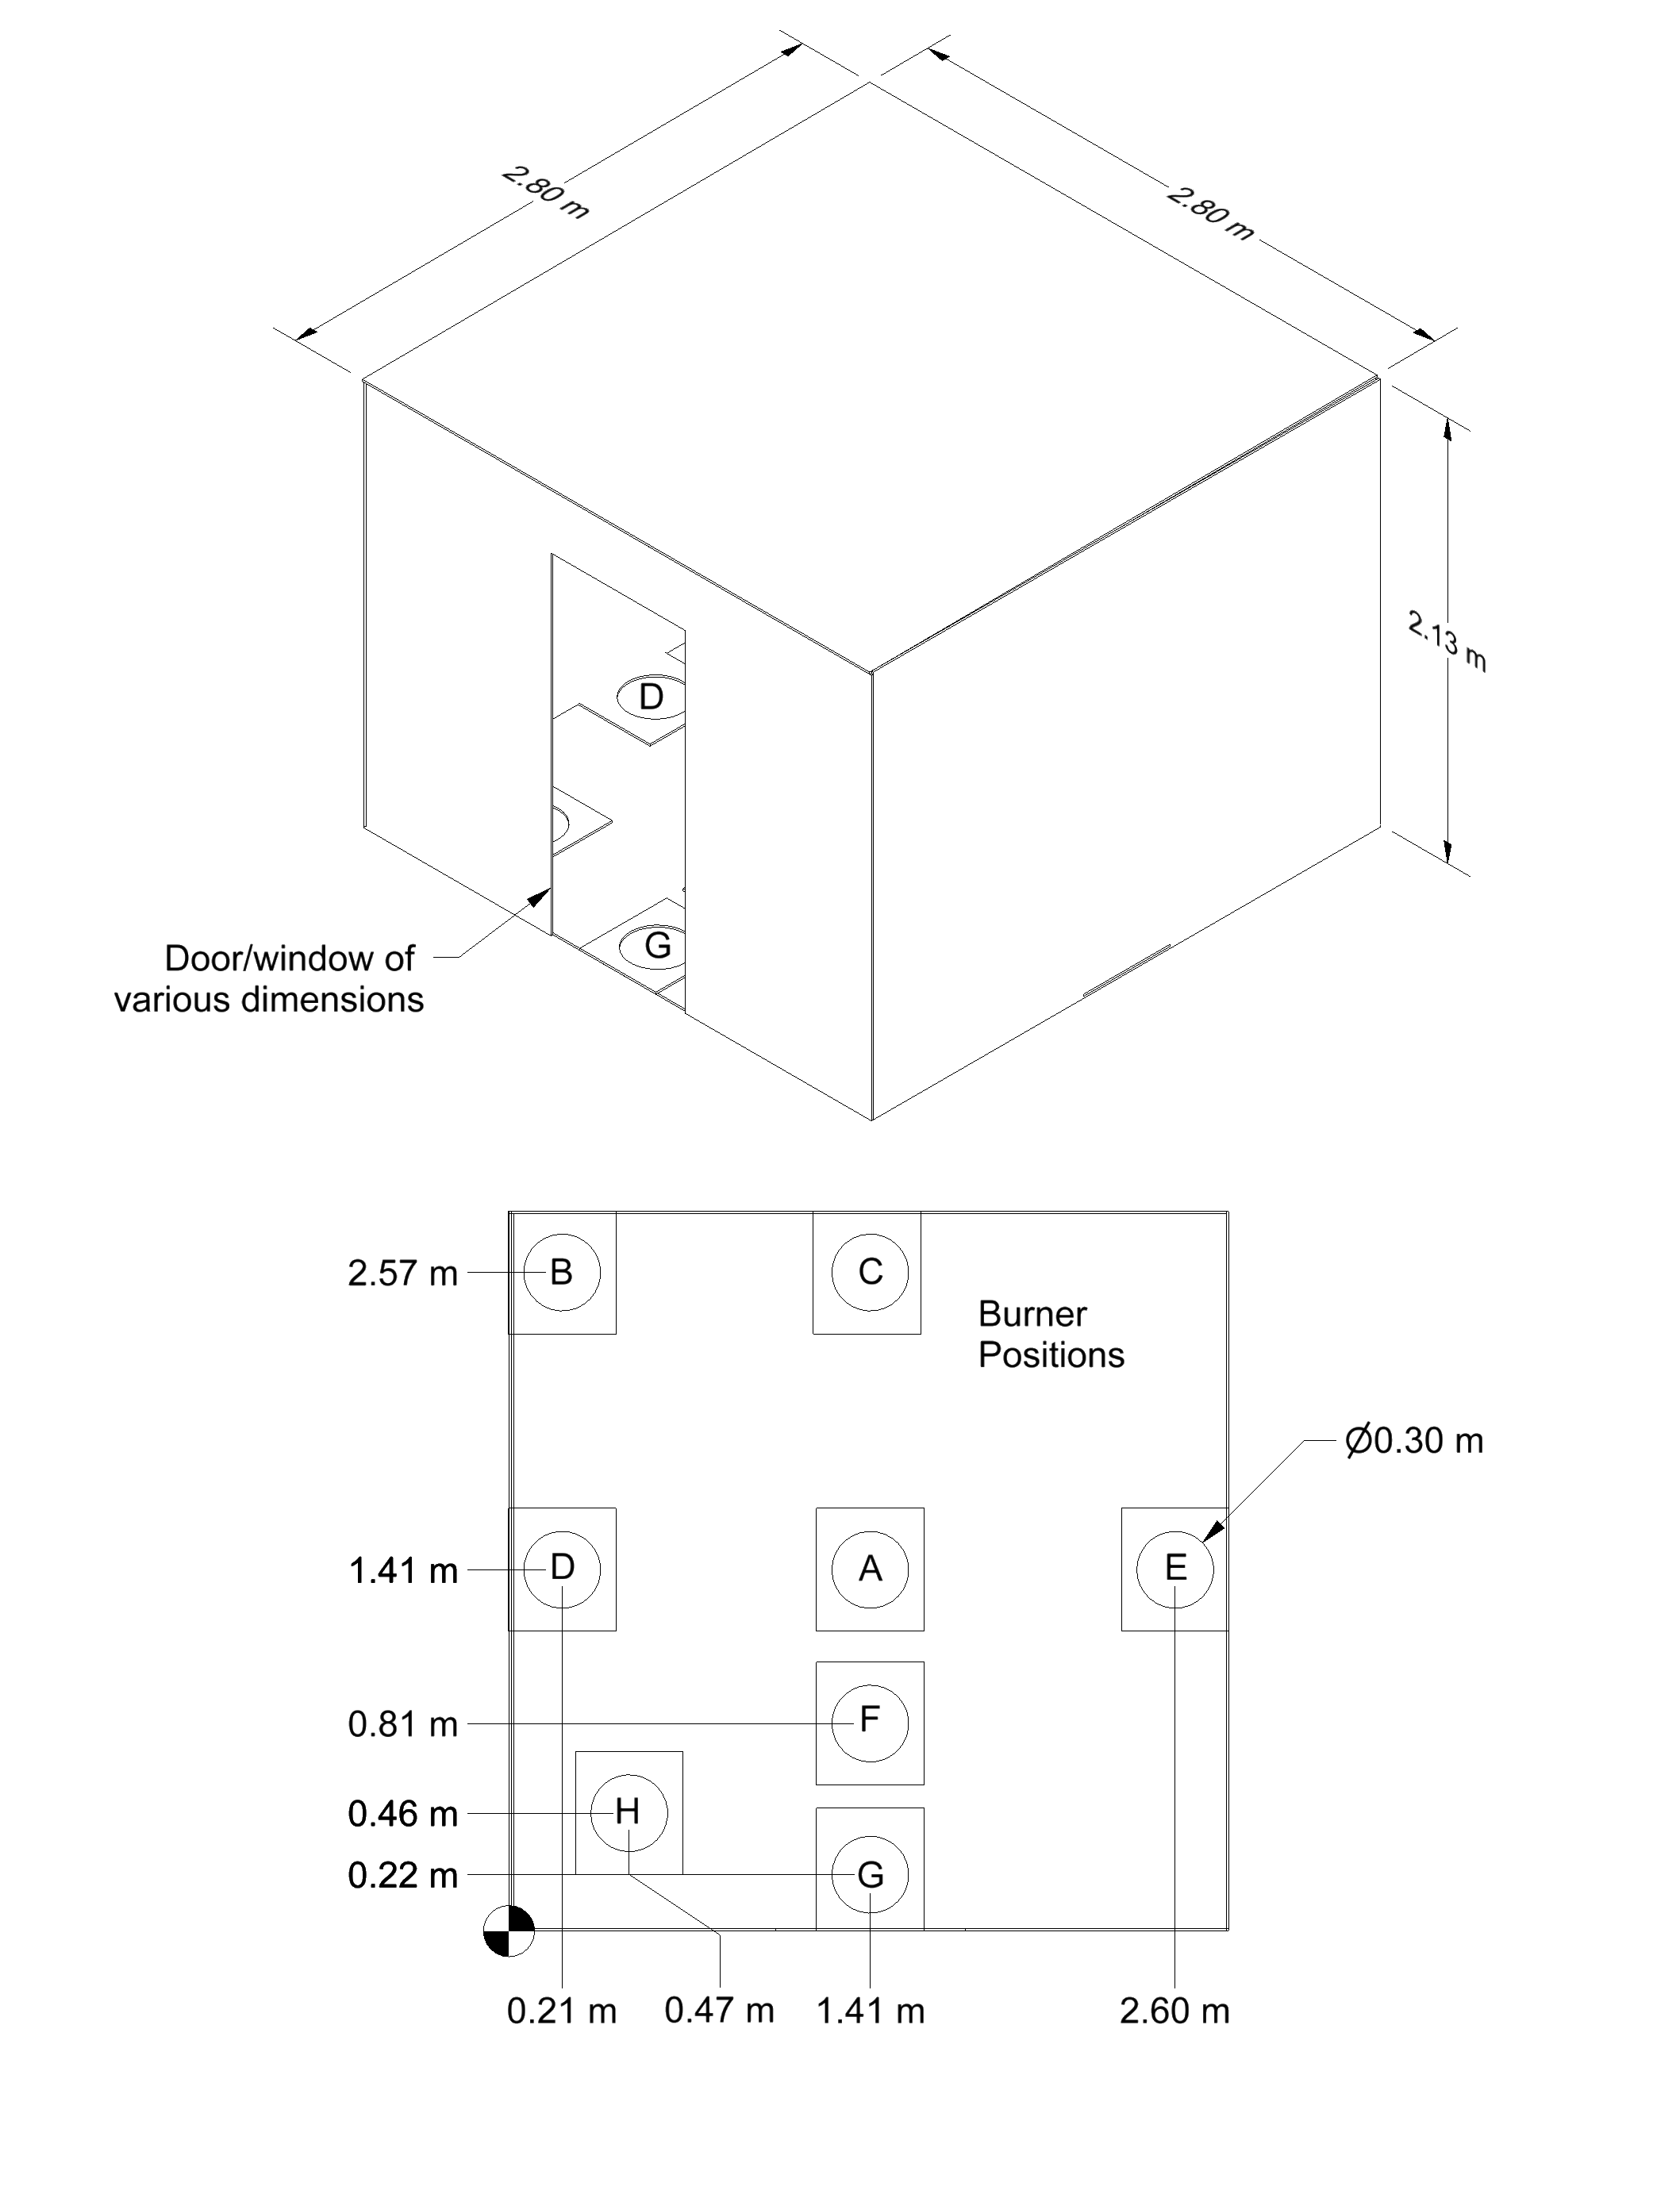
\includegraphics[width=\textwidth]{FIGURES/Steckler_Compartment/Steckler_Room_Drawing.png}
\caption{Geometry of the Steckler Compartment Experiments.}
\label{Steckler_ Drawing}
\end{figure}

\section{UL/NFPRF Sprinkler, Vent, and Draft Curtain Study}
\label{UL_NFPRF_Description}

In 1997, a series of 34 heptane spray burner experiments was conducted at the Large Scale Fire Test Facility at Underwriters Laboratories
(UL) in Northbrook, Illinois~\cite{Sheppard:1}. The experiments were divided into two test series. Series I consisted of 22 4.4~MW experiments. Series~II consisted
of 12 10~MW experiments. The objective of the experiments was to characterize the temperature and flow field for fire
scenarios with a controlled heat release rate in the presence of sprinklers, draft curtains, and smoke \& heat vents.
The Large Scale Fire Test Facility at UL contains a 37~m by 37~m (120~ft by 120~ft) main fire test cell, equipped with a 30.5~m by 30.5~m (100~ft by
100~ft) adjustable height ceiling. The layout of the experiments is shown in Figs.~\ref{layout} and \ref{burnerlayoutA}.

\begin{figure}[p]
\begin{center}
\setlength{\unitlength}{.05416667in}
\begin{picture}(120,120)

\linethickness{1.mm} \put(0,0){\framebox(120,120)[tc]{North Wall}} \linethickness{.5mm} \put(10,10){\framebox(100,100)[tc]{Adjustable Height
Ceiling}}

\thinlines \put(117,67){\vector(0,-1){67}} \put(117,73){\vector(0, 1){47}} \put(117,70){\makebox(0,0){$120'$}} \put(113,57){\vector(0,-1){47}}
\put(111,110){\line(1,0){4.}} \put(111, 10){\line(1,0){4.}} \put(113,63){\vector(0, 1){47}} \put(113,60){\makebox(0,0){$100'$}}
\put(30.9,12.83){\dashbox{1}(67.1,71.17)[tc]{Draft Curtains}} \put(27.9,40){\vector(0,-1){27.17}} \put(27.9,46){\vector(0, 1){38.0}}
\put(25.9,84.){\line(1,0){4.}} \put(25.9,12.83){\line(1,0){4.}} \put(27.9,43){\makebox(0,0){$71'2''$}} \put(64.0,87.){\vector(-1,0){33.1}}
\put(72.0,87.){\vector( 1,0){26.0}} \put(30.9,85.){\line(0,1){4.}} \put(98.0,85.){\line(0,1){4.}} \put(68.0,87.){\makebox(0,0){$67'1''$}}

\put(16.0,87.){\vector(-1,0){6.}} \put(24.0,87.){\vector( 1,0){6.92}} \put(20.0,87.){\makebox(0,0){$20'11''$}} \put(101.,87.){\vector(-1,0){3.}}
\put(107.,87.){\vector( 1,0){3.}} \put(104.,87.){\makebox(0,0){$12'$}}

\put(27.9,100){\vector(0,1){10.}} \put(27.9,94){\vector(0,-1){10.}} \put(27.9,97){\makebox(0,0){$26'$}}

\put(27.9,8){\vector(0,1){2.}} \put(27.9,8){\line(1,0){3.}} \put(30.9,8){\makebox(0,0)[l]{$2'10''$}}

\put(55.08,14.83){\line(-1,0){2.}} \put(54.08,16.83){\vector(0,-1){2.}} \put(54.08,7.83){\vector(0,1){5.}} \put(54.08,7.83){\line(1,0){3.}}
\put(57.08,7.83){\makebox(0,0)[l]{$2'$}}

\put(85.08,24.83){\line(0,-1){2.}} \put(95.08,24.83){\line(0,-1){2.}} \put(93.08,23.83){\vector(1,0){2.}} \put(87.08,23.83){\vector(-1,0){2.}}
\put(103.00,23.83){\vector(-1,0){5.}} \put(103.00,23.83){\line(0,-1){3.}} \put(103.00,20.83){\makebox(0,0)[ct]{$2'11''$}}
\put(90.08,23.83){\makebox(0,0)[c]{$10'$}}

\thicklines \put(78.08,55.83){\framebox(4,8){ }}

\put(78.58,58.33){\framebox(3,3)[c]{A}} \put(78.58,68.33){\framebox(3,3)[c]{B}} \put(88.58,58.33){\framebox(3,3)[c]{C}}
\put(58.58,38.33){\framebox(3,3)[c]{D}}

\thinlines

\multiput(35.08,14.83)(0,10){7}{\circle*{.8}} \multiput(45.08,14.83)(0,10){7}{\circle*{.8}} \multiput(55.08,14.83)(0,10){7}{\circle*{.8}}
\multiput(65.08,14.83)(0,10){7}{\circle*{.8}} \multiput(75.08,14.83)(0,10){7}{\circle*{.8}} \multiput(85.08,14.83)(0,10){7}{\circle*{.8}}
\multiput(95.08,14.83)(0,10){7}{\circle*{.8}} \tiny \put(35.48,15.23){98} \put(45.48,15.23){91} \put(55.48,15.23){84} \put(65.48,15.23){81}
\put(75.48,15.23){78} \put(85.48,15.23){75} \put(95.48,15.23){72} \put(35.48,25.23){99} \put(45.48,25.23){92} \put(55.48,25.23){85}
\put(65.48,25.23){82} \put(75.48,25.23){79} \put(85.48,25.23){76} \put(95.48,25.23){73} \put(35.48,35.23){100} \put(45.48,35.23){93}
\put(55.48,35.23){86} \put(65.48,35.23){83} \put(75.48,35.23){80} \put(85.48,35.23){77} \put(95.48,35.23){74} \put(35.48,45.23){101}
\put(45.48,45.23){94} \put(55.48,45.23){87} \put(65.48,45.23){62} \put(75.48,45.23){58} \put(85.48,45.23){54} \put(95.48,45.23){50}
\put(35.48,55.23){102} \put(45.48,55.23){95} \put(55.48,55.23){88} \put(65.48,55.23){63} \put(75.48,55.23){59} \put(85.48,55.23){55}
\put(95.48,55.23){51} \put(35.48,65.23){103} \put(45.48,65.23){96} \put(55.48,65.23){89} \put(65.48,65.23){64} \put(75.48,65.23){60}
\put(85.48,65.23){56} \put(95.48,65.23){52} \put(35.48,75.23){104} \put(45.48,75.23){97} \put(55.48,75.23){90} \put(65.48,75.23){65}
\put(75.48,75.23){61} \put(85.48,75.23){57} \put(95.48,75.23){53} \put(70.08,49.83){\makebox(0,0)[c]{68}} \put(70.08,59.83){\makebox(0,0)[c]{69}}
\put(70.08,69.83){\makebox(0,0)[c]{70}} \put(80.08,49.83){\makebox(0,0)[c]{67}} \put(90.08,49.83){\makebox(0,0)[c]{66}}
\put(90.08,69.83){\makebox(0,0)[c]{71}}

\multiput(80.08,56.83)(0,1){7}{\circle*{.2}} \put(80.58,62.83){\line(1,0){22.5}} \put(104.,62.83){\makebox(0,0)[l]{43}}
\put(104.,61.33){\makebox(0,0)[l]{44}} \put(104.,59.83){\makebox(0,0)[l]{45}} \put(104.,58.33){\makebox(0,0)[l]{46}}
\put(104.,56.83){\makebox(0,0)[l]{47}} \put(104.,55.33){\makebox(0,0)[l]{48}} \put(104.,53.83){\makebox(0,0)[l]{49}}

\normalsize

\end{picture}
\end{center}
\caption[Plan view of the UL/NFPRF Experiments, Series~I.] {Plan view of the UL/NFPRF Experiments, Series~I. The sprinklers are indicated by the solid circles and
are spaced 3~m apart. The number beside each sprinkler location indicates the channel number of the nearest thermocouple. The vent dimensions
are 4~ft by 8~ft. The boxed letters A, B, C and D indicate burner positions. Corresponding to each burner position is a vertical array of
thermocouples. Thermocouples 1--9 hang 7, 22, 36, 50, 64, 78, 92, 106 and 120~in from the ceiling, respectively, above Position A. Thermocouples 10
and 11 are positioned above and below the ceiling tile directly above Position B, followed by 12--20 that hang at the same levels below the ceiling
as 1--9. The same pattern is followed at Positions C and D, with thermocouples 21--31 at C and 32--42 at D.}
\label{layout}
\end{figure}


\begin{figure}[p]
\begin{center}
\setlength{\unitlength}{.054166in}
\begin{picture}(120,120)

\linethickness{1mm}
\put(0,0){\framebox(120,120)[tc]{ }}
\put(60,118){\makebox(0,0){North Wall}}
\put(60,  2){\makebox(0,0){South Wall}}

\linethickness{.5mm}
\put(10,10){\framebox(100,100)[tl]{ }}

\thinlines
\put(117,67){\vector(0,-1){67}}
\put(117,73){\vector(0, 1){47}}
\put(117,70){\makebox(0,0){$120'$}}
\put(113,57){\vector(0,-1){47}}
\put(113,63){\vector(0, 1){47}}
\put(113,60){\makebox(0,0){$100'$}}
\put(10.0,86.0){\dashbox{1}(30.0,24.0)[tl]{ }}
\put(40.,10.5){\dashbox{1}(69.5,75.5)[tl]{              }}

\thicklines
\put(48.,16.){\framebox(4,8){ }}
\put(48.,67.){\framebox(4,8){ }}
\put(28.,67.){\framebox(4,8){ }}
\put(98.,67.){\framebox(4,8){ }}
\put(98.,16.){\framebox(4,8){ }}

\large
\put(68.5,49.5){\dashbox{.5}(3,3)[c]{D}}
\put(48.5,69.5){\dashbox{.5}(3,3)[c]{A}}
\put(48.5,79.5){\dashbox{.5}(3,3)[c]{B}}
\put(58.5,59.5){\dashbox{.5}(3,3)[c]{C}}
\put(38.5,54.5){\dashbox{.5}(3,3)[c]{E}}
\put(38.5,84.5){\dashbox{.5}(3,3)[c]{F}}
\normalsize

\multiput(15,11)(0,10){10}{\circle*{.8}}
\multiput(25,11)(0,10){10}{\circle*{.8}}
\multiput(35,11)(0,10){10}{\circle*{.8}}
\multiput(45,11)(0,10){10}{\circle*{.8}}
\multiput(55,11)(0,10){10}{\circle*{.8}}
\multiput(65,11)(0,10){10}{\circle*{.8}}
\multiput(75,11)(0,10){10}{\circle*{.8}}
\multiput(85,11)(0,10){10}{\circle*{.8}}
\multiput(95,11)(0,10){10}{\circle*{.8}}
\multiput(105,11)(0,10){10}{\circle*{.8}}

\end{picture}
\end{center}
\caption[Plan view of the UL/NFPRF Experiments, Series~II ]
{Plan view of the UL/NFPRF Experiments, Series~II. The boxed letters A, B, C, D, E and F indicate burner positions. The sprinklers are indicated
by the solid circles and are spaced 10~ft apart. The branch lines run
north to south. The vents are 4~ft by 8~ft. }
\label{burnerlayoutA}
\end{figure}



\begin{description}
\item[Ceiling:] The ceiling was raised to a height of 7.6~m and instrumented with thermocouples and other measurement devices. The ceiling was constructed of
0.6~m by 1.2~m by 1.6~cm UL fire-rated Armstrong Ceramaguard (Item 602B) ceiling tiles. The manufacturer reported the
thermal properties of the material to be: specific heat 753 J/(kg$\cdot$K), thermal conductivity
0.0611~W/(m$\cdot$K), and density 313~kg/m$^3$.
\item[Draft Curtains:] Sheet metal, 1.2~mm thick and 1.8~m deep, was suspended from the ceiling for 16 of the 22 Series~I tests, enclosing an area of about 450~m$^2$ and 49 sprinklers.
The curtains were in place for all of the Series~II tests.
\item[Sprinklers:] Central ELO-231 (Extra Large Orifice) uprights were used for all the tests. The orifice diameter of this sprinkler is reported by the manufacturer to be
nominally 1.6~cm (0.64~in), the reference actuation temperature is reported by the manufacturer to be 74$^\circ$C (165$^\circ$F). The RTI (Response Time
Index) and C-factor (Conductivity factor) were reported by UL to be 148~(m$\cdot$s)$^\ha$ and 0.7~(m/s)$^\ha$, respectively~\cite{Sheppard:1}.
When installed, the sprinkler deflector was located 8~cm below the ceiling. The thermal
element of the sprinkler was located 11~cm below the ceiling. The sprinklers were installed with nominal 3~m by 3~m (exact 10~ft by 10~ft) spacing in a
system designed to deliver a constant 0.34~L/(s$\cdot$m$^2$) (0.50 gpm/ft$^2$) discharge density when supplied by a 131~kPa (19~psi) discharge
pressure
\item[Vent:] UL-listed double leaf fire vents with steel covers and steel curb were installed in the adjustable height ceiling in the position shown in
Figs.~\ref{layout} and \ref{burnerlayoutA}. The vent is designed to open manually or automatically. The vent doors were recessed into the ceiling about 0.3~m (1~ft).
\item[Heat Release Rate:] The heptane spray burner consisted of a 1~m by 1~m square of 1.3~cm pipe supported by four cement blocks 0.6~m off the floor.
Four atomizing spray nozzles were used to provide a free spray of heptane that was then ignited. For all but one of the Series~I tests, the total heat release
rate from the fire was manually ramped up following a ``t-squared'' curve to a steady-state in 75~s
(150~s was used in Test I-16). The fire was ramped to 10~MW in 75~s for the Series~II tests. The fire growth curve was followed until a specified fire size was
reached or the first sprinkler activated. After either of these events, the fire size was maintained at that level until conditions reached roughly a
steady state, i.e., the temperatures recorded near the ceilings remained steady and no more sprinkler activations occurred.
The heat release rate from the burner was confirmed by placing it under the large product calorimeter at UL, ramping up the flow of heptane in the
same manner as in the tests, and measuring the total and convective heat release rates. It was found that the convective heat release rate was
0.65~$\pm$~0.02 of the total.
\item[Instrumentation:] The instrumentation for the tests consisted of thermocouples, gas analysis equipment, and pressure transducers. The locations of the instrumentation
are referenced in the plan view of the facility (Fig.~\ref{layout}).
Temperature measurements were recorded at 104 locations. Type K 0.0625~in diameter Inconel sheathed thermocouples were positioned to measure (i)
temperatures near the ceiling, (ii) temperatures of the ceiling jet, and (iii) temperatures near the vent.
\end{description}

\section{UL/NIST Vent Experiments}
\label{UL_NIST_Vents_Description}

In 2012, the Fire Fighting Technology Group at NIST conducted experiments at Underwriters Laboratories (UL) in Northbrook, Illinois, to assess the change in compartment temperature due to the opening of one or two 1.2~m square ceiling vents \cite{Opert:2012}. Four experiments were conducted using a natural gas burner in a 6.1~m by 4.3~m by 2.4~m compartment with a single door opening. The fires ranged in size from 500~kW to 2~MW, and the vents were opened and closed such that during the four experiments there were 31 discrete time intervals in which model predictions could be compared to quasi-steady conditions. The compartment contained two vertical arrays of thermocouples, and the door and vents were instrumented with thermocouples and bi-directional velocity probes. Only the thermocouple data has been used in the validation study. A diagram of the compartment is displayed in Figure~\ref{UL_NIST_Drawing}. The major test parameters are listed in Table~\ref{UL_NIST_Table}.

\begin{figure}
\begin{center}
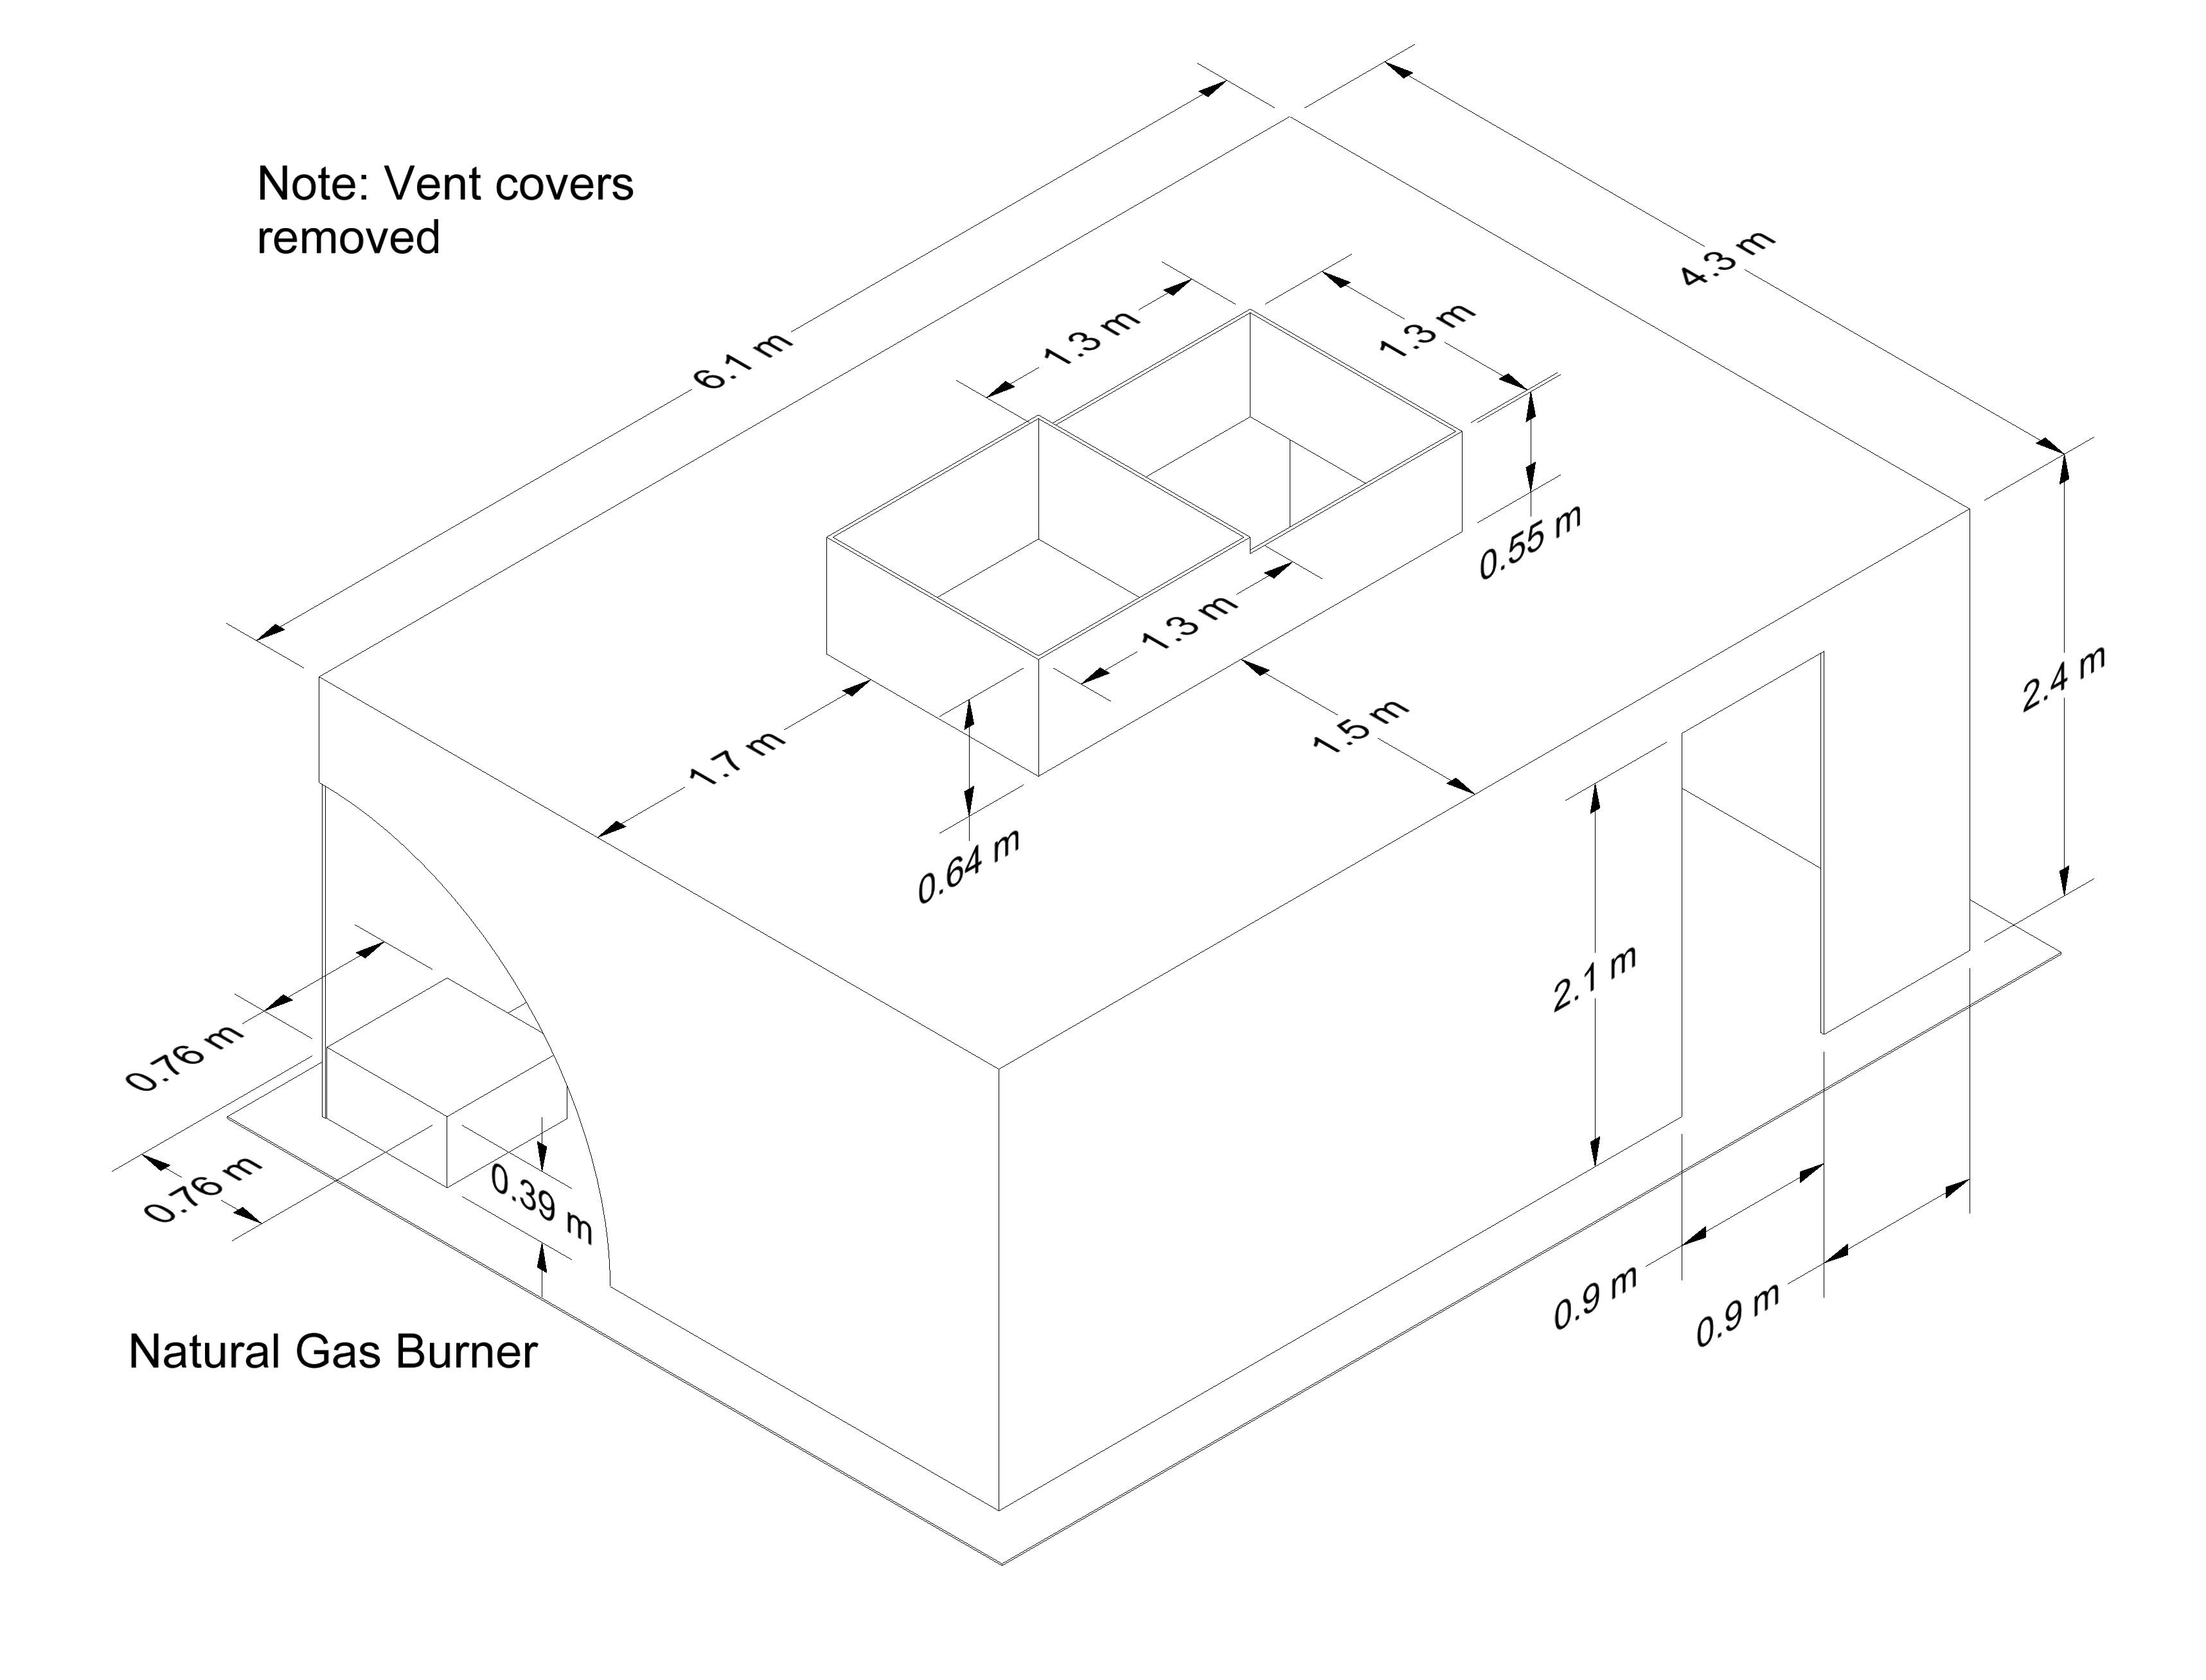
\includegraphics[width=6.5in]{FIGURES/UL_NIST_Vents/UL_NIST_Vents_Drawing}
\end{center}
\caption{Geometry of the UL/NIST Experiments.}
\label{UL_NIST_Drawing}
\end{figure}


\begin{table}[h!]
\caption[Summary of UL/NIST Vent experiments]{Summary of UL/NIST Vent experiments. Note that the 31 ``experiments'' are actually discrete time intervals during the course of four separate fires.}
\begin{center}
\begin{tabular}{|c|c|c|c||c|c|c|c|}
\hline
Exp.    & End Time  & HRR           &  No. of   & Exp.    & End Time  & HRR           &  No. of           \\
No.     & (s)       & (kW)          & Vents     & No.     & (s)       & (kW)          & Vents             \\ \hline \hline
\multicolumn{4}{|c||}{Fire 1}                   & \multicolumn{4}{|c|}{Fire 3}                            \\ \hline
1       & 1215      & 430           & 0         & 14      & 453       & 476           & 0                 \\ \hline
2       & 1840      & 430           & 1         & 15      & 816       & 476           & 1                 \\ \hline
3       & 2168      & 430           & 2         & 16      & 1153      & 476           & 2                 \\ \hline
4       & 2474      & 430           & 0         & 17      & 1640      & 1002          & 0                 \\ \hline
5       & 2955      & 1011          & 0         & 18      & 1936      & 1002          & 1                 \\ \hline
6       & 3170      & 1011          & 1         & 19      & 2233      & 1002          & 2                 \\ \hline
7       & 3604      & 1011          & 2         & \multicolumn{4}{|c|}{Fire 4}                            \\ \hline
8       & 3840      & 1011          & 0         & 20      & 519       & 1011          & 0                 \\ \hline
9       & 4153      & 2188          & 0         & 21      & 967       & 1011          & 1                 \\ \hline
10      & 4284      & 2188          & 1         & 22      & 1325      & 1011          & 2                 \\ \hline
\multicolumn{4}{|c||}{Fire 2}                   & 23      & 1559      & 470           & 2                 \\ \hline
11      & 565       & 2144          & 0         & 24      & 1653      & 470           & 1                 \\ \hline
12      & 833       & 2144          & 1         & 25      & 2013      & 470           & 0                 \\ \hline
13      & 931       & 2144          & 2         & 26      & 2411      & 470           & 1                 \\ \hline
\multicolumn{4}{|r||}{}                         & 27      & 2910      & 470           & 2                 \\ \cline{5-8}
\multicolumn{4}{|r||}{}                         & 28      & 3399      & 2188          & 2                 \\ \cline{5-8}
\multicolumn{4}{|r||}{}                         & 29      & 3586      & 2188          & 0                 \\ \cline{5-8}
\multicolumn{4}{|r||}{}                         & 30      & 3803      & 2188          & 1                 \\ \cline{5-8}
\multicolumn{4}{|r||}{}                         & 31      & 4035      & 2188          & 2                 \\ \hline
\end{tabular}
\end{center}
\label{UL_NIST_Table}
\end{table}

\section{USN High Bay Hangar Experiments}

The U.S. Navy sponsored a series of 33 tests within two hangars examining fire detection and sprinkler activation in response to spill fires in large enclosures \cite{Gott:1997, Davis:2000}. Experiments were conducted using JP-5 and JP-8 fuels in two Navy high bay aircraft hangars located in Naval Air Stations in Barber's Point, Hawaii and Keflavik, Iceland.

The Hawaii tests were conducted in a 15~m high hangar measuring 97.8~m in length and 73.8~m in width. Of the 13 tests conducted in the facility 11 were conducted in pans ranging from .09~m$^2$ to 4.9~m$^2$ in area with heat release rates varying from 100~kW to 7.7~MW. The burner was placed in the center of the room on a scale that continuously recorded the pans weight. The facility was equipped with a number of detection devices including thermocouples, electronic smoke and spot heat detectors, projected beam smoke detectors, combination UV/IR optical flame detectors, line-type heat detectors, as well as sprinklers. Measurements were recorded at a large number of locations allowing for a through profile of compartment behavior.

It was suspected that fire plume behavior and response of detection devices in a cold building may not have been well replicated by the experiments held in the warm hangar in Hawaii. The Iceland tests were conducted under a 22~m barrel vaulted ceiling in a hangar measuring 45.7~m by 73.8~m. 22 tests in total were conducted. The majority of these tests fires burned JP-5 fuel with the remainder burning JP-8. The jet fuel fires ranged in size from .06~m$^2$ to 20.9~m$^2$ and in heat release rate from 100~kW to approximately 33~MW. The facility was equipped similarly to the Hawaii hangar.

\section{Vettori Flat Ceiling Experiments}

Vettori~\cite{Vettori:1} analyzed a series of 45 experiments conducted at NIST that were intended to compare the effects of different ceiling configurations on the activation times of quick response residential pendent sprinklers. The two ceiling configurations used consisted of an obstructed ceiling, with parallel beams 0.038~m wide by 0.24~m deep placed 0.41~m on center, and a smooth ceiling configuration, in which the beams were covered by a sheet of gypsum board.  In addition to the two ceiling configurations, there were also three fire growth rates and three burner locations used -- a total of 18 test configurations. The fire growth rate was provided by a computer controlled methane gas burner to mimic a standard t-squared fire growth rate with either a slow, medium, or fast ramp up. The burner was placed in a corner of the room, then against an adjacent wall, and then in a location removed from any wall. Measurements were taken to record sprinkler activation time, temperatures at varying heights and locations within the room, and the ceiling jet velocities at several other locations.  A diagram of the test structure is displayed in Figure~\ref{Vettori_Drawing}.

\begin{figure}[\figoptions{b}]
\begin{center}
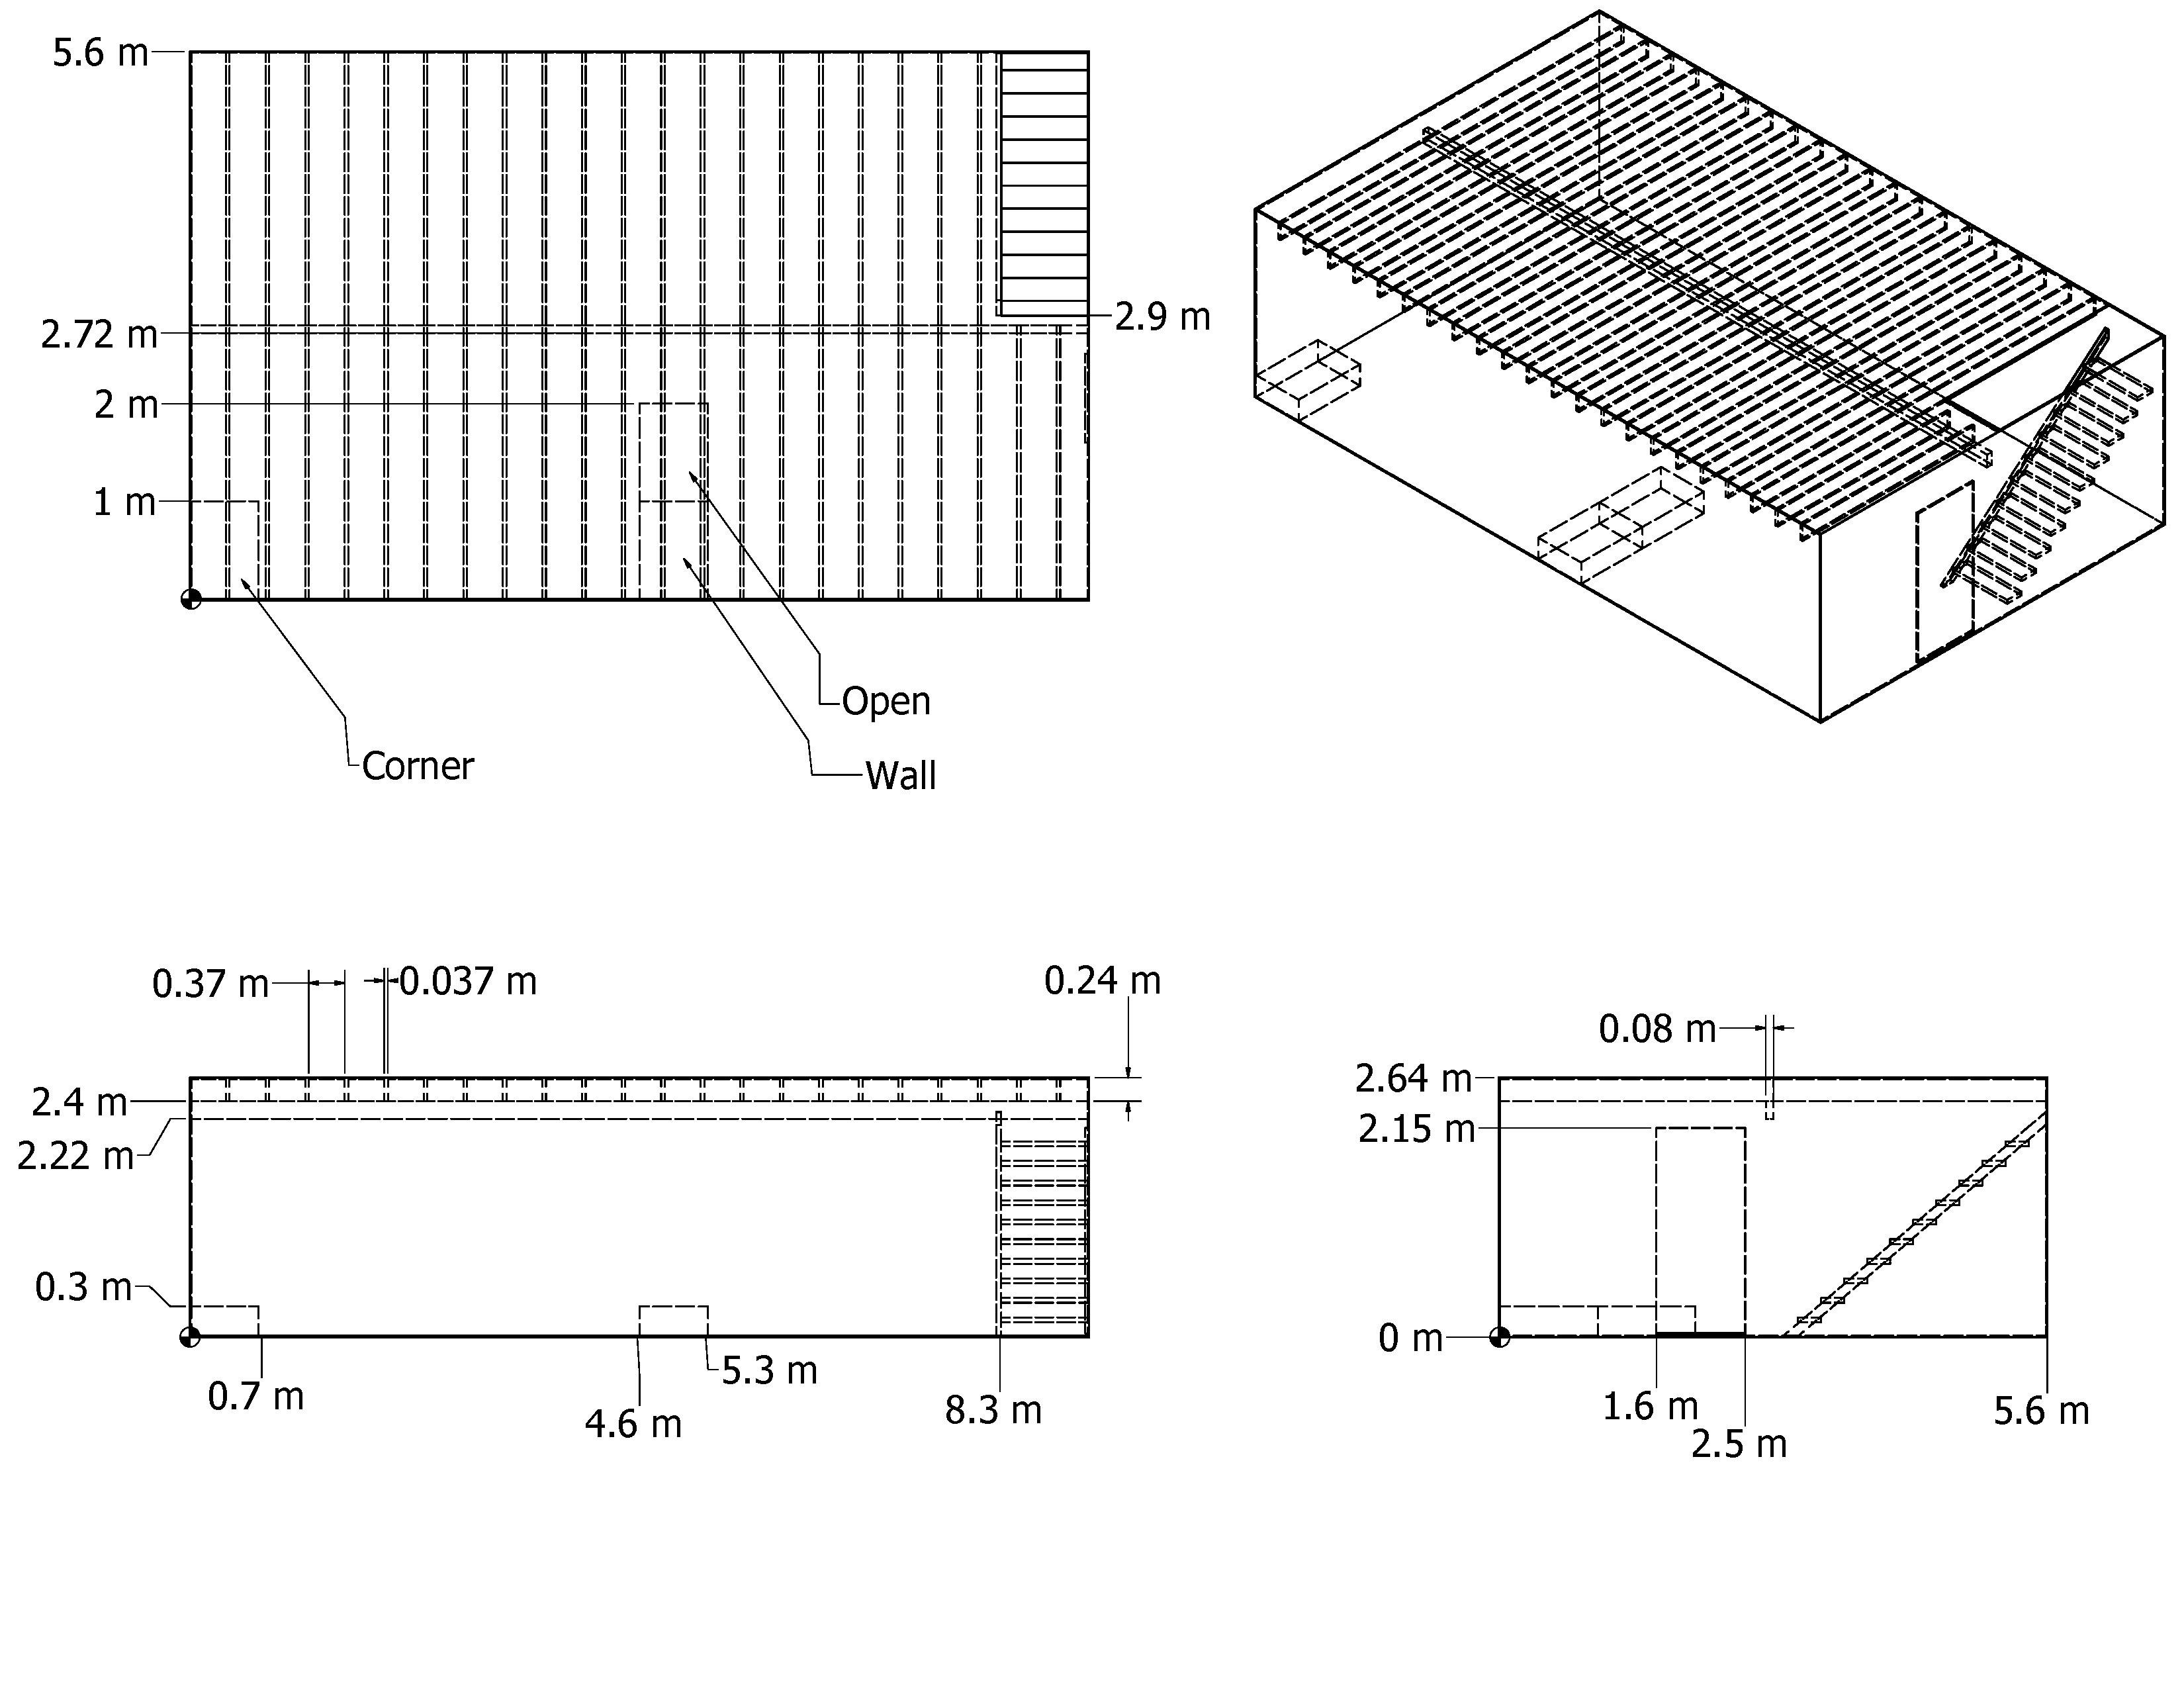
\includegraphics[width=6.5in]{FIGURES/Vettori_Flat/Vettori_Flat_Ceiling}
\end{center}
\caption[Geometry of the Vettori Flat Ceiling compartment]{Geometry of the Vettori Flat Ceiling compartment.}
\label{Vettori_Drawing}
\end{figure}

\section{VTT Large Hall Tests}

The experiments are described in reference~\cite{Hostikka:2001}. The series consisted three unique fire scenarios with replications for a total of 8 experiments. The experiments were undertaken to study the movement of smoke in a large hall with a sloped ceiling. The tests were conducted inside the VTT Fire Test Hall, with dimensions of 19 m high by 27 m long by 14 m wide. Figure \ref{fig:VTT_cutaway} shows the important features of the test hall. Figure \ref{fig:VTT_Schematic} shows detailed plan, side and perspective schematic diagrams of the experimental arrangement. Each test involved a single heptane pool fire, ranging from 2~MW to 4~MW. Figure \ref{fig:VTT_2MW_fire} is a photo of a 2~MW fire. Four types of measurements were used in the present evaluation -- the hot gas layer temperature and depth, average flame height and the plume temperature. Three vertical arrays of thermocouples, plus two thermocouples in the plume, were compared to model simulation results. The hot gas layer temperature and height were reduced from an average of the three thermocouple arrays using a standard algorithm. The ceiling jet temperature was not considered, because the ceiling in the test hall is not flat, and the model algorithm is not appropriate for these conditions.

\begin{figure}[\figoptions{b}]
\begin{center}
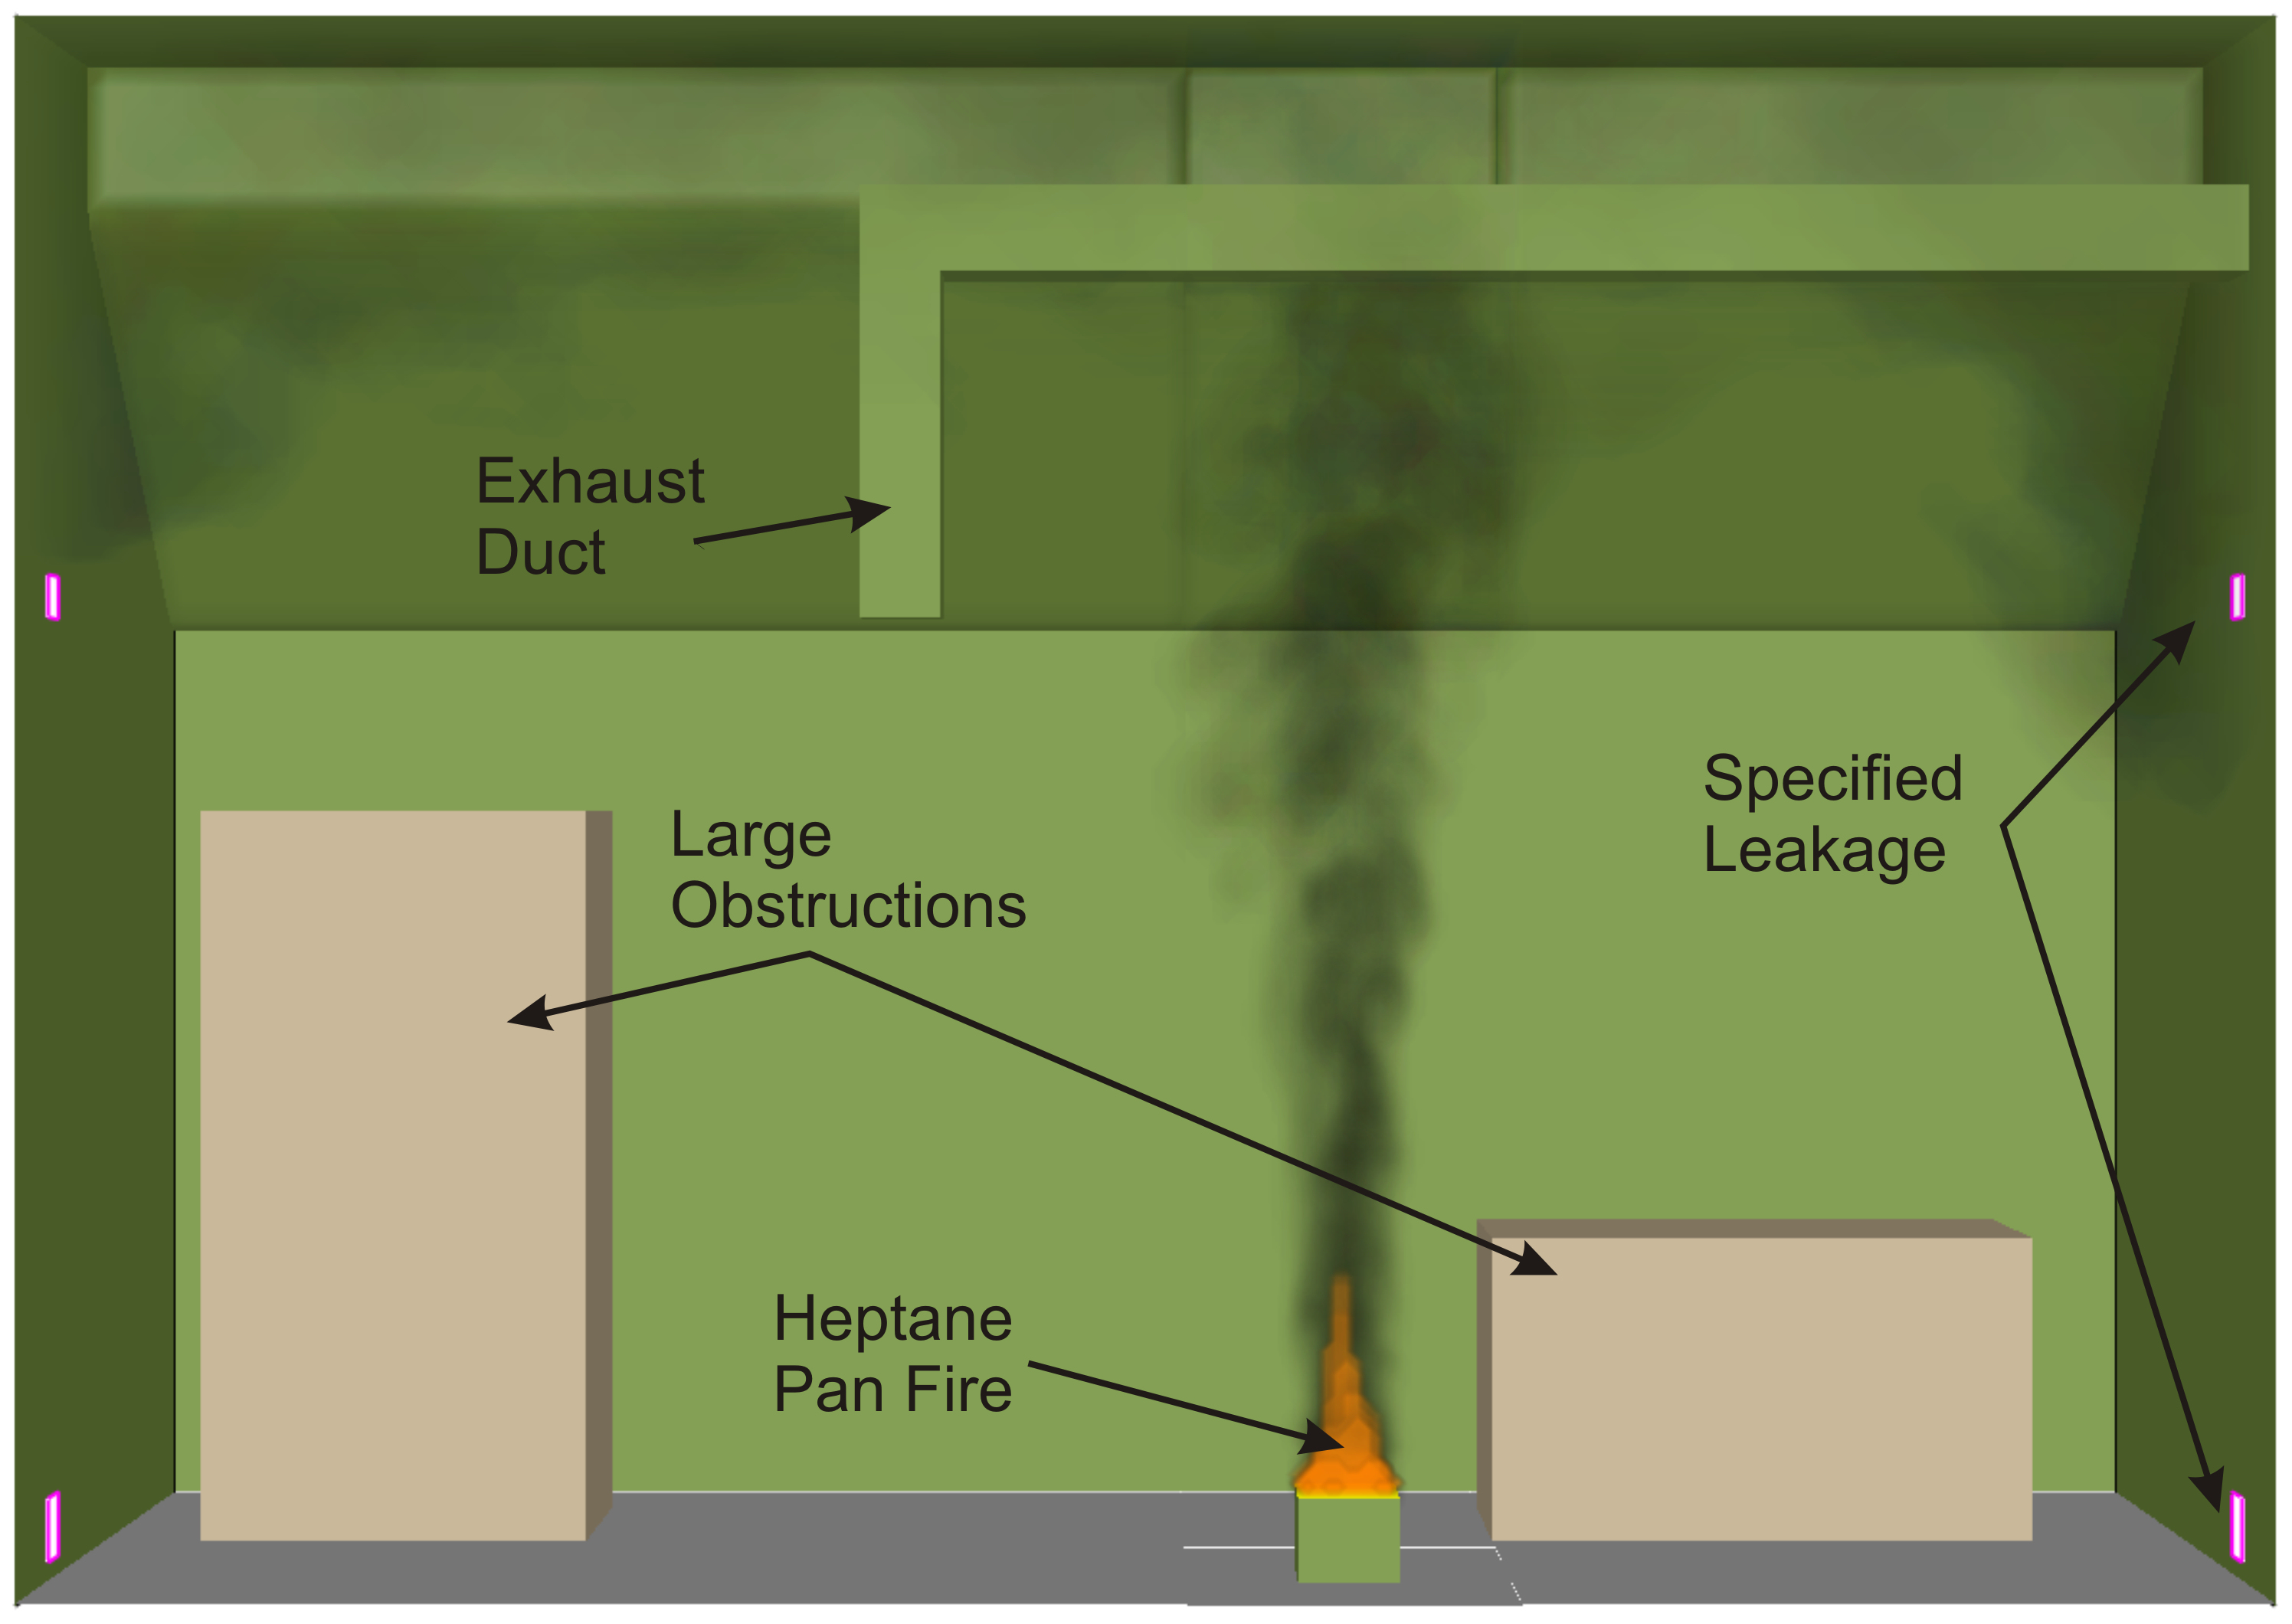
\includegraphics[width=5.0in]{FIGURES/VTT/VTT_Cut_Away}\\
\end{center}
\caption{Cut-Away View of Case 2 of the VTT Large Hall Tests.}
 \label{fig:VTT_cutaway}
\end{figure}

\begin{figure}[\figoptions{b}]
\begin{center}
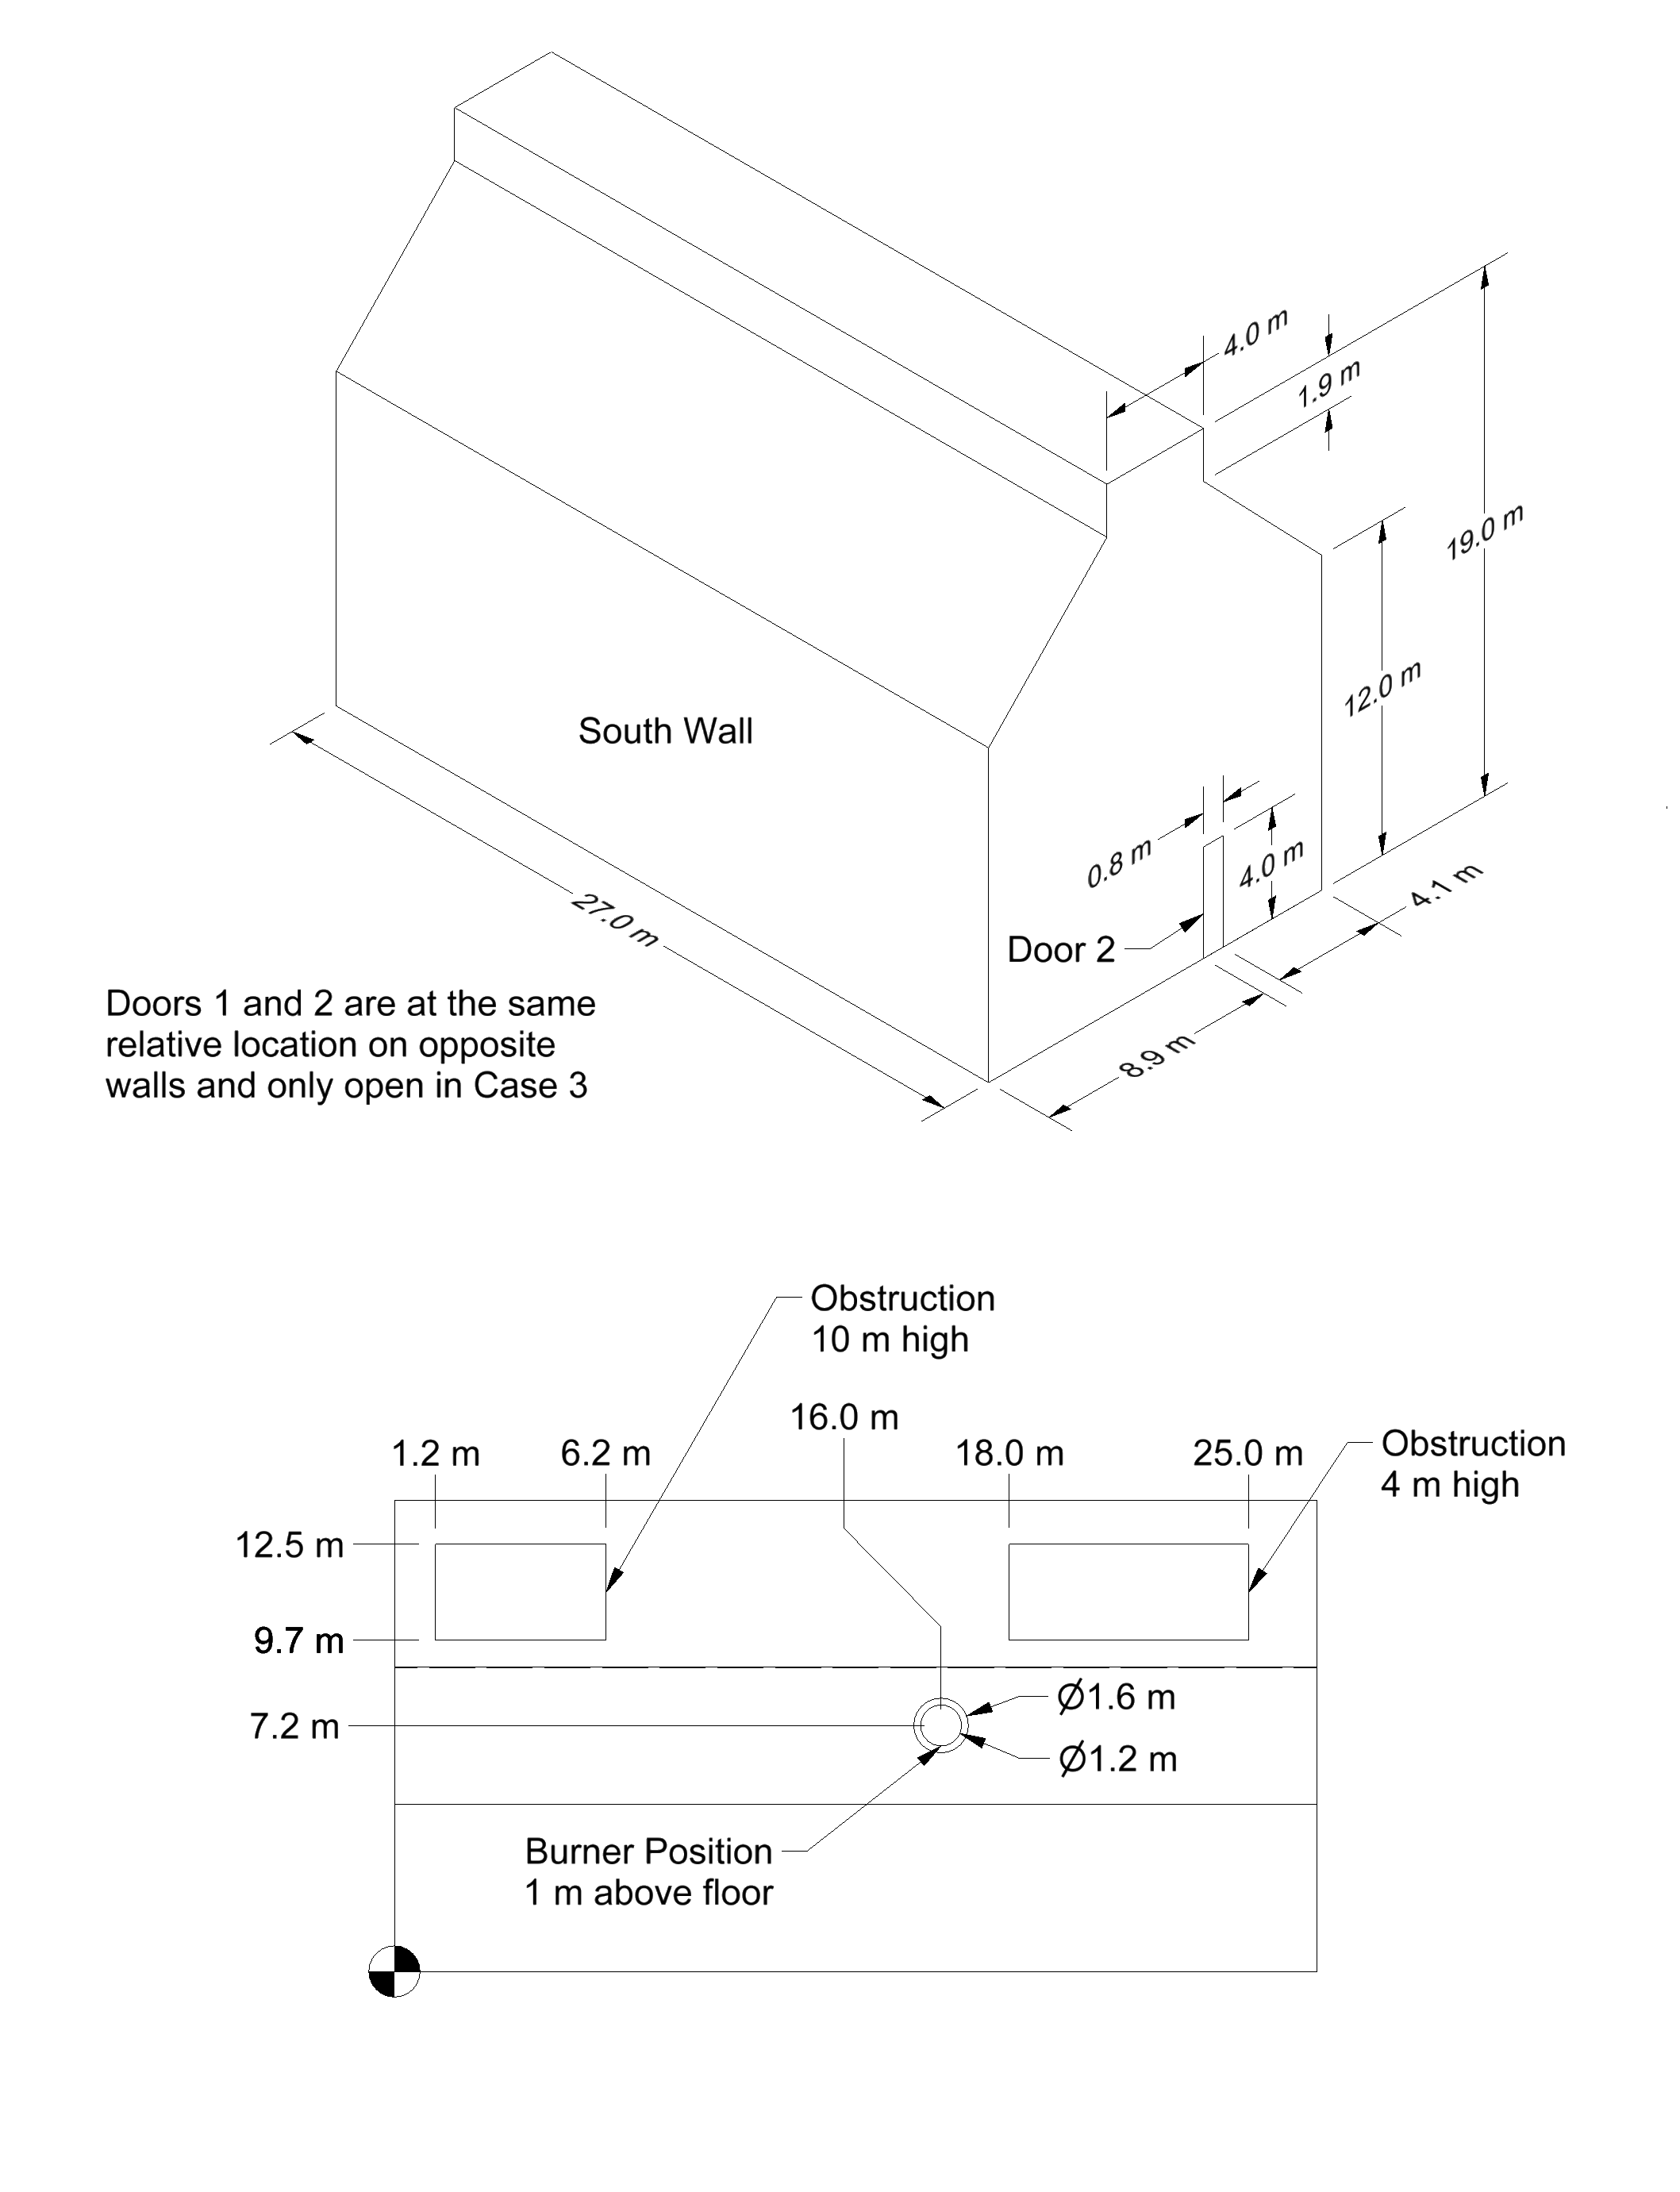
\includegraphics[width=6.5in]{FIGURES/VTT/VTT_Drawing}\\
\end{center}
\caption{Plan, side and perspective schematic drawings of the experimental arrangement of the VTT large hall fire tests, including the fuel pan}
 \label{fig:VTT_Schematic}
\end{figure}

\begin{figure}[\figoptions{b}]
\begin{center}
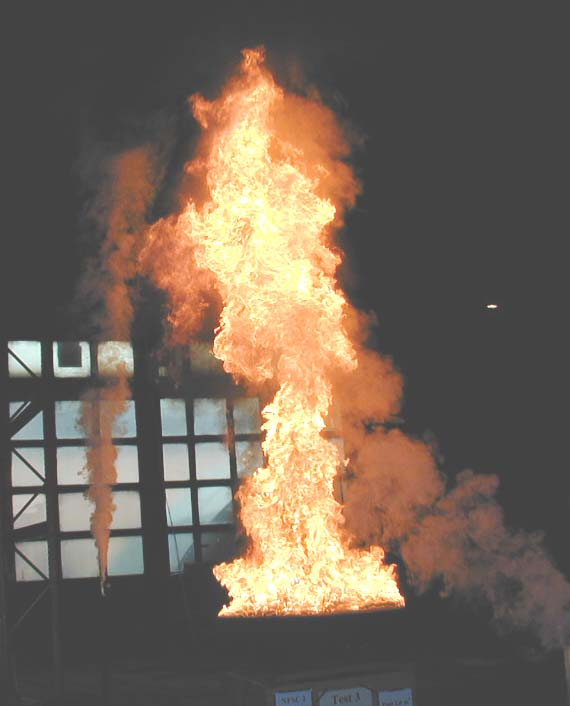
\includegraphics[width=3.0in]{FIGURES/VTT/VTT_2MW_fire}\\
\end{center}
\caption{Photo of a 2 MW heptane fire during the VTT large hall tests. Photo provided by Simo Hostikka, VTT.}
 \label{fig:VTT_2MW_fire}
\end{figure}

The VTT test report lacks some information needed to model the experiments, so some information was based on private communications with the principal investigator, Simo Hostikka. Details used to conduct the model simulations is presented in reference \cite{NRCNUREG1824}, including information on the fire, the compartment, and the ventilation.

The walls and ceiling of the test hall consist of a 1 mm thick layer of sheet metal on top of a 5 cm layer of mineral wool. The floor was constructed of concrete. The report does not provide thermal properties of these materials. Thermophysical properties of the materials that were used in the simulations are given in table \ref{tab:VTT_Thermals}.

\begin{table}[h!]
\begin{center}
\caption{Thermophysical Properties for VTT Large Hall Tests}
\label{tab:VTT_Thermals}
\vspace{0.1in}
\begin{tabular}{|l|c|c|c|c|c|}
\hline
Material & Conductivity & Specific Heat & Density & Thickness & Emissivity\\
 & W/m$^{\circ}$C & J/kg$^{\circ}$C & kg/m$^3$ & m & \\ \hline
\hline
Steel ICFMP BE2 & 54 &        425 &       7850 &      0.001 &       0.95  \\ \hline
Concrete ICFMP BE2 &          2 &        900 &        230 &       0.15 &       0.95 \\ \hline
\end{tabular}
\end{center}
\end{table}

In Cases 1 and 2, all doors were closed, and ventilation was restricted to leakage through the building envelope. Precise information on air infiltration during these tests is not available. The scientists who conducted the experiments recommend a leakage area of about 2~m$^2$, distributed uniformly throughout the enclosure. By contrast, in Case 3, the doors located in each end wall (Doors 1 and 2, respectively) were open to the external ambient environment. These doors are each 0.8 m wide by 4 m high, and are located such that their centers are 9.3 m from the south wall. The test hall had a single mechanical exhaust duct, located in the roof space, running along the center of the building. This duct had a circular section with a diameter of 1 m, and opened horizontally to the hall at a distance of 12 m from the floor and 10.5 m from the west wall. Mechanical exhaust ventilation was operational for Case 3, with a constant volume flow rate of 11 m$^3$/s drawn through the 1 m diameter exhaust duct.

Each test used a single fire source with its center located 16 m from the west wall and 7.4 m from the south wall. For all tests, the fuel was heptane in a circular steel pan that was partially filled with water. The pan had a diameter of 1.17 m for Case 1 and 1.6 m for Cases 2 and 3. In each case, the fuel surface was 1 m above the floor. The trays were placed on load cells, and the HRR was calculated from the mass loss rate. For the three cases, the fuel mass loss rate was averaged from individual replicate tests. In the HRR estimation, the heat of combustion (taken as 44.6 kJ/g) and the combustion efficiency for n-heptane was used.  In this report, a combustion efficiency of 0.85 $\pm$ 0.12 (or $\pm$ 14 \%) was used for the VTT pool fire tests. Due to the relatively large value of the uncertainty associated with the combustion efficiency the uncertainty in HRR is dominated by the uncertainty in the combustion efficiency. Uncertainty in the mass loss rate measurement also contributed to the overall uncertainty, and the uncertainty in HRR was estimated as 15 \% \cite{NRCNUREG1824}. Figure \ref{fig:VTT_HRR} show the prescribed HRR as a function of time during Cases 1 to 3, respectively. The radiative fraction was assigned a value of 0.35 \cite{NRCNUREG1824}, similar to many smoky hydrocarbons \cite{Hamins:1991}. The relative combined expanded (2$\sigma$) uncertainty in this parameter was assigned a value of $\pm$ 20 \%, which is typical of uncertainty values reported in the literature for this parameter. Further details of the model inputs used for these simulations are included in reference \cite{NRCNUREG1824}.

\begin{figure}[p]
\begin{center}
\begin{tabular}{c}
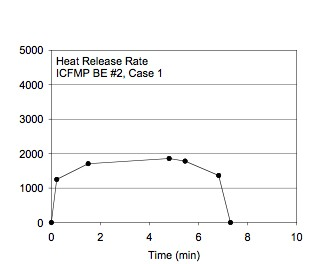
\includegraphics[width=2.6in]{FIGURES/VTT/VTT_Case1_HRR} \\
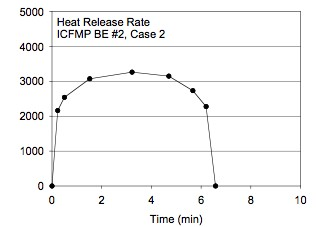
\includegraphics[width=2.6in]{FIGURES/VTT/VTT_Case2_HRR} \\
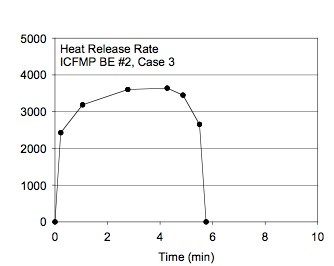
\includegraphics[width=2.6in]{FIGURES/VTT//VTT_Case3_HRR}
\end{tabular}
\end{center}
\caption{Prescribed Heat Release Rate as a Function of Time for VTT Large Hall Tests.} \label{fig:VTT_HRR}
\end{figure}

\clearpage
\clearpage

\section{WTC Spray Burner Test Series}

As part of its investigation of the World Trade Center disaster, the Building and Fire Research Laboratory at NIST conducted several series of fire experiments to both gain insight into the
observed fire behavior and also to validate FDS for use in reconstructing the fires. The first series of experiments involved a relatively simple compartment with a liquid spray burner and
various structural elements with varying amounts of sprayed fire-resistive materials (SFRM). A diagram of the compartment is shown in figure~\ref{WTC_Drawing}.
A complete description of the experiments can be found in the NIST WTC report NCSTAR~1-5B~\cite{NIST_NCSTAR_1-5B}.
The overall enclosure was rectangular, as were the vents and most of the obstructions. The compartment walls and ceiling were made of 2.54~cm thick marinite. The manufacturer provided the thermal properties of the material used in the calculation. The density was 737~kg/m$^3$, conductivity 0.12~W/m/K. The specific heat ranged from 1.17~kJ/kg/K at 93~$^\circ$C to
1.42~kJ/kg/K at 425~$^\circ$C. This value was assumed for higher temperatures.
The steel used to construct the column and truss flanges was 0.64~cm thick.  The density of the steel was assumed to be 7,860~kg/m$^3$; its specific heat 0.45~kJ/kg/K.

Two fuels were used in the tests. The properties of the fuels were obtained from measurements made on a series of unconfined burns that are referenced in the test report.
The first fuel was a blend of heptane isomers, C$_7$H$_{16}$. Its soot yield was set at a constant 1.5~\%. The second fuel was a mixture (40~\% - 60~\% by volume) of toluene, C$_7$H$_8$,
and heptane. Because FDS only considers the burning of a single hydrocarbon fuel, the mixture was taken to be C$_7$H$_{12}$ with a soot yield of 11.2~\%.
The radiative fraction for the heptane blend was 0.44; for the heptane/toluene mixture it was 0.39.
The heat release rate of the simulated burner was set to that which was measured in the experiments with the fire placed on the floor at the center of the fire pan.

\begin{figure}[p]
\begin{center}
\includegraphics[width=6.5in]{FIGURES/WTC/WTC_Drawing}
\end{center}
\caption[Geometry of the WTC Experiments]{Geometry of the compartment used for the WTC Experiments.}
\label{WTC_Drawing}
\end{figure}


\section{Summary of Experiments}

\label{experiment_summary}

Table~\ref{Test_Parameters} presents a summary of all the experiments described in this chapter in terms of parameters commonly used in fire protection engineering. This ``parameter space'' outlines the range of applicability of the validation studies performed to date. In other words, if this guide is to be cited as justification for using FDS to simulate a given fire scenario, that scenario must be similar to these experiments in the sense of having comparable physical parameters. These parameters are explained below:

\begin{description}
\item[Heat Release Rate, $\dQ$,] is the range of peak heat release rates of the fires in the test series.
\item[Fire Diameter, $D$,] is the equivalent diameter of the base of the fire, calculated $D=\sqrt{4A/\pi}$, where $A$ is the area of the base.
\item[Ceiling Height, $H$,] is the distance from floor to ceiling.
\item[Fire Froude Number, $\dot{Q}^*$,] is a useful non-dimensional quantity for plume correlations and flame height estimates. \be \dot{Q}^* = \frac{\dot{Q}}{\rho_\infty c_p T_\infty \sqrt{gD} D^2} \ee It is essentially the ratio of the fuel gas exit velocity and the buoyancy-induced plume velocity. Jet fires are characterized by large Froude numbers. Typical accidental fires have a Froude number near unity.
\item[Flame Height relative to Ceiling Height, $L_{\rm f}/H$,] is a convenient way to express the physical size of the fire relative to the size of the room. The height of the visible flame, based on Heskestad's correlation, is estimated by: \be L_{\rm f} = D \, \left( 3.7 \, (\dot{Q}^*)^{2/5} - 1.02 \right) \ee
\item[Global Equivalence Ratio, $\phi$,] is the ratio of the mass flux of fuel to the mass flux of oxygen into the compartment, divided by the stoichiometric ratio. \be \phi = \frac{\dm_{\rm f}}{r\, \dm_{\hbox{\tiny O$_2$}}} \equiv  \frac{\dQ \; \hbox{(kW)}}{13,100 \; \hbox{(kJ/kg)} \; \dm_{\hbox{\tiny O$_2$}} } \quad ; \quad  \dm_{\hbox{\tiny O$_2$}} = \left\{
     \begin{array}{r@{\quad:\quad}l}
      \ha \, 0.23 \, A_0 \sqrt{H_0} & \hbox{Natural Ventilation} \\
      0.23 \, \rho \, \dot{V}       & \hbox{Mechanical Ventilation} \end{array} \right. \ee Here, $r$ is the stoichiometric ratio, $A_0$ is the area of the compartment opening, $H_0$ is the height of the opening, $\rho$ is the density of air, and $\dot{V}$ is the volume flow of air into the compartment. If $\phi<1$, the compartment is considered ``well-ventilated'' and if $\phi>1$, the compartment is considered ``under-ventilated.''
\item[Compartment Aspect Ratios, $W/H$ and $L/H$,] indicate if the compartment is shaped like a hallway, typical room, or vertical shaft.
\item[Relative Distance along the Ceiling, $r_{\rm cj}/H$,] indicates the distance from the fire plume of a sprinkler, smoke detector, etc., relative to the compartment height, $H$.
\item[Relative Distance from the Fire, $r_{\rm rad}/D$,] indicates whether a ``target'' is near or far from the fire.
\end{description}

\newpage \thispagestyle{empty}
\begin{sidewaystable}[p]
\caption{Summary of important experimental parameters. }
\begin{center}
\begin{tabular}{|l|c|c|c|c|c|c|c|c|c|c|c|c|}
\hline
                                        & $\dot{Q}$     & $D$           & $H$    &                               &                                  &               &             &             &                       &                       \\
\rb{Test Series}               & (kW)              & (m)            & (m)          & \rb{$\dot{Q}^*$}  & \rb{$L_{\rm f}/H$}  & \rb{$\phi$}   & \rb{$W/H$}  & \rb{$L/H$}  & \rb{$r_{\rm cj}/H$}   & \rb{$r_{\rm rad}/D$}  \\ \hline \hline
ATF Corridors                   & 50 -- 500       & 0.5             & 2.4        & 0.3 -- 3.3                & 0.3 -- 0.9                  & 0.0 -- 0.1      & 0.8               & 7.1              & 0.8 -- 6.0                   &                                       \\ \hline
FM/SNL                             & 470 -- 516    & 0.9             & 6.1         & 0.6 -- 2.4               & 0.3 -- 0.6                 & 0.0 -- 0.2      & 2.0                & 3.0             & 0.2 -- 0.3                   &                                        \\ \hline
iBMB*                                & 3500, 400    & 1.13, 0.79  & 5.7, 5.6 & 2.4, 0.7                 &   0.6, 0.4                & 0.6, 0.1         & 0.6              & 0.6               &                                   &                                        \\ \hline
LLNL Enclosure                 & 50 -- 400       & 0.6             & 4.5        & 0.2 -- 1.5               & 0.1 -- 0.4                & 0.1 -- 0.4      & 0.9                & 1.3              & 0.3 -- 1.0                  &                                        \\ \hline
NBS Multi-Room                & 110               & 0.3             & 2.4        & 1.5                         & 0.5                          &                      & 1.0                & 5.1             &                                  &                                          \\ \hline
NBS Single-Compartment & 2900 -- 7000 & 1.1 -- 1.7   & 2.4        & 1.7 -- 2.3               &1.1                            &                      & 1.0                & 1.5              &                                  &                                           \\ \hline
%NIST Seven-Story            & 1130              &  0.7            & 2.6       & 2.2                         & 1.1                          &                       & 0.7                & 5.6             &                                   &                                           \\ \hline
NIST/NRC                         & 350 -- 2200   & 1.0              & 3.8      & 0.3 -- 2.0              & 0.3 -- 1.0                 & 0.0 -- 0.3      & 1.9                & 5.7              & 0.3 -- 2.1                  & 2.0 -- 4.0                          \\ \hline
NIST Smoke Alarm            & 100 -- 350     & 1.0             & 2.4       & 0.1 -- 0.3               & 0.2 -- 0.5                 &                      & 1.7                & 8.3              & 1.3 -- 8.3                  &                                          \\ \hline
SP AST                             & 450                & 0.3              & 2.4      & 6.1                         & 1.1                           & 0.1              & 1.0                  & 1.5               &                                  &                                         \\ \hline
Steckler                            & 31.6 -- 158    & 0.3              & 2.1      & 0.8 -- 3.8              & 0.3 -- 0.7                  & 0.0 -- 0.6    & 1.3                 & 1.3                &                                  &                                         \\ \hline
UL/NFPRF                        & 4400 -- 10000 & 1.0             & 7.6      & 4.0 -- 9.1              & 0.7 -- 1.0                  & Open           & 4.9                 & 4.9                & 0.6 -- 3.9                 &                                         \\ \hline
UL/NIST Vents                 & 500 -- 2000     & 0.9              & 2.4     & 0.7 -- 2.6             & 0.8 -- 1.6                  & 0.2 -- 0.6    & 1.8                 & 2.5                & 1.0 -- 2.3                  &                                       \\ \hline
USN Hawaii                     & 100 -- 7700      & 0.3 -- 2.5    & 15      & 0.7 -- 1.3              & 0.1 -- 0.4                  & Open          & 4.9                  & 6.5                & 0 -- 1.2                    &                                          \\ \hline
USN Iceland                    & 100 -- 15700   & 0.3 -- 3.4    & 22      & 0.7 -- 1.3             & 0.0 -- 0.3                  & Open           & 2.1                 & 3.4                & 0 -- 1.0                     &                                       \\ \hline
Vettori Flat                      & 1055                & 0.7             & 2.6     & 2.5                      & 1.1                            & 0.3               & 2.1                 & 3.5                & 0.8 -- 2.9                  &                                       \\ \hline
VTT Large Hall                 & 1860 -- 3640   & 1.4 -- 1.8    & 19     & 0.7                      & 0.2                             & 0                  & 1.0                 & 1.4                & 0 -- 0.6                      &                                    \\ \hline
WTC                               & 1970 -- 3240   & 1.6              & 3.8    & 0.6 -- 0.9             & 0.8 -- 1.1                  & 0.3 -- 0.5     & 0.9                  & 1.8               & 0.0 -- 0.8                   & 0.3 -- 1.3                    \\ \hline
\end{tabular}
\end{center}
* Where two values are present, the first is for the test from iBMB test \#4 and the second is from iBMB test \#5.
\label{Test_Parameters}
\nopagebreak
\end{sidewaystable}




\noindent
